\documentclass[a4paper, 11pt]{article}

%--------------------------------------------------------------------
%--- Title, author, date
%--------------------------------------------------------------------

\newcommand{\docauthor}{Martins Bruveris}
\newcommand{\docdate}{2016 $|$ November $|$ 24}
\newcommand{\docclass}{MA2712}
\newcommand{\doctitle}{Problems}

%--------------------------------------------------------------------
%--- Input custom header
%--------------------------------------------------------------------

%--------------------------------------------------------------------
%--- Notes to myself
%--------------------------------------------------------------------

% TODO: Tautasdziesma
% TODO: Figure out how vertical space works in title page
%       Clean up code for title page
% TODO: Add section numbers to pdf bookmarks
% TODO: Change document class to book to have two parts
%       Part 1 - problems
%       Part 2 - solutions
%       Both in one document
% TODO: Work on page geometry

% Need gnuplot to compile this
% TODO: Add id to plots, so we can compile without gnuplot,
%       see TikZ manual p.329.
% TODO: Change figuretable to use tabu
%       Avoid globally resetting \tabcolsep
% TODO: Tables for local extrema look bad
% 
% TODO: Sect. 10, choose better functions to integrate over
%       rectangles
% TODO: Check for consistent usage of alignenum
% 
%--------------------------------------------------------------------
%--- Loading packages
%--------------------------------------------------------------------

\PassOptionsToPackage{dvipsnames}{xcolor} % Is loaded by TikZ                                

\usepackage{amsmath,amsthm,textcomp}

\usepackage[charter,expert]{mathdesign}   % Bitstream Charter font, 
                                          % as recommended by Aleksey
\usepackage[scaled=.96,osf]{XCharter}     % Matches the size used in math
\usepackage{microtype}                    % Typographical improvements
\usepackage{bm}

\usepackage[T1]{fontenc}  % These three packages load Times fonts
% \usepackage{mathptmx}
% \usepackage{tgtermes} 

% \usepackage{newtxtext}  % Other fonts to consider
% \usepackage{newtxmath}

\usepackage[utf8]{inputenc}
\usepackage{graphicx}

\usepackage{enumitem}                     % Customize lists
% \usepackage{enumerate}                  
\usepackage{geometry}                     % Customize page geometry
% \usepackage{showframe}                    % To show page geometry
\usepackage{fancyhdr}                     % Custom headers and footers
\usepackage{lastpage}                     % To show "Page 1 / 20"

\usepackage{tikz}                         % For drawing figures

\usepackage{exsheets}                     % For problem/solution environments
\usepackage{wrapfig}                      % To let text wrap around a figure
\usepackage{adjustbox}                    % For wrapfigure inside enumerate
\usepackage{ifthen}                       % iften for defining commands
\usepackage{siunitx}                      % To typeset units
\usepackage{tabu}                         % tabu environment for tables
\usepackage{tasks}                        % tasks environment for horizontal lists
\usepackage{nth}
\usepackage[savepos]{zref}                % For align in enumerate workaround
\usepackage{etoolbox}                     % For parameter toggles
\usepackage{xcolor}                       % For red title

\usepackage[style=numeric, minnames=3,
            doi=false, url=false, isbn=false,
            firstinits=true,
            sortcites=true,
            backend=biber]{biblatex}      % For bibliographies

%--------------------------------------------------------------------
%--- Pdf options
%--------------------------------------------------------------------

\usepackage[
  pdftitle={\docclass{} -- \doctitle}, 
  pdfauthor={\docauthor},
  colorlinks=true,
  linkcolor=blue,
  urlcolor=blue,
  citecolor=blue,
  bookmarks=true,
  bookmarksopenlevel=2]{hyperref}

\usepackage[inline]{asymptote}            % For asymptote graphics

%--------------------------------------------------------------------
%--- Global page geometry and layout
%--------------------------------------------------------------------

\geometry{
%  total={210mm,297mm},
  left=25mm,
  right=25mm,
  bindingoffset=0mm, 
  top=20mm,
  bottom=20mm
}

\fancyhf{}
\renewcommand{\headrulewidth}{0.5pt}
\fancyhead[L]{\textsc{\docclass}}
\fancyhead[C]{\textsc{\doctitle}}
\fancyhead[R]{\textsc{\docdate}}
\renewcommand{\footrulewidth}{0.5pt}
\fancyfoot[L]{\textsc{\docauthor}}
\fancyfoot[C]{}
\fancyfoot[R]{\textsc{Page \thepage\ /\ \pageref*{LastPage}}}

\setlength{\headheight}{14pt} % Was necessary, warning otherwise

\fancypagestyle{firstpage}{
  \fancyhf{}
  \renewcommand{\footrulewidth}{0pt}
  \fancyfoot[L]{}
  \fancyfoot[C]{}
  \fancyfoot[R]{}
  \renewcommand{\headrulewidth}{0mm}
}

\pagestyle{fancy}

\author{\docauthor}
\date{\docdate}
\title{\docclass{} -- \doctitle}

% Custom Title
\newcommand{\linia}{\rule{\linewidth}{0.5pt}}

\makeatletter
\renewcommand{\maketitle}{
\begin{center}
\vspace{2ex}
{\huge \textsc{\@title}}
\vspace{1ex}
\\
\linia\\
\textsc{\@author} \hfill \textsc{\@date}
\vspace{4ex}
\end{center}
}
\makeatother

%--------------------------------------------------------------------
%--- Microtype settings
%--- Source: microtype documentation
%--------------------------------------------------------------------

\microtypesetup{expansion=alltext, step=1}
\microtypesetup{kerning=true}

\DeclareMicrotypeSet*[protrusion]
  { doc }
  { encoding = {*, TS1, OMS},
    family   = {rm*, tt*},
    size     = {footnotesize, small, normalsize} }
\SetProtrusion
  { encoding = OMS,
    family   = mdbch }
  { "68 = {400, },  % \langle
    "69 = { ,400} } % \rangle
\DeclareMicrotypeSet*[kerning]
  { doc }
  { encoding = T1,
    family   = blg, % typewriter font and ...
    font     = * }  % French sample in section \ref{sub:kerning}
\SetExtraKerning
  { encoding = T1,
    family   = blg }
  { _ = {100,100} } % underscores shouldn't touch

%--------------------------------------------------------------------
%--- Global parameters and commands
%--------------------------------------------------------------------

\linespread{1.2}

\everymath{\displaystyle}

% Table to typeset tikz figures; parameter is number of columns
\newenvironment{figuretable}[2][1em]
  {
    \begin{tabular}{*{#2}{c@{\hspace{#1}}}}
  }
  {
    \end{tabular}
  }

% A better solution should be found for this...
\tabcolsep=0pt

% Used to adjust vertical height for wrapfigure inside enumerate
\newlength{\strutheight}
\settoheight{\strutheight}{\strut}

\renewcommand{\labelenumi}{(\alph{enumi})} % Use letters for enumerate

\settasks{counter-format=(tsk[a])} % Use letters for tasks lists
\settasks{label-width={1.5em}}

\let\six=\si % \si is defined by package siunitx, but we use it for \sigma

% Pagebreak after each problem section
\newboolean{sectionnewpage}
\setboolean{sectionnewpage}{false}

% For printing difficulty level
\newcommand{\difficulty}[1]{(#1)}

% Bibliography
\addbibresource{bibliography.bib}

% Align in enumerate environment
% Source: tex.stackexchange.com/questions/9394
\newenvironment{alignenum}{%
  $\begin{aligned}[t]
}{%
  \end{aligned}$
}
% This one has centered formulas
% \newenvironment{alignenum}{%
%   \hfill$\begin{aligned}[t]
% }{%
%   \end{aligned}$\hfill\null
% }

\newcounter{dummy} % necessary for correct hyperlinks (to index, bib, etc.)

%--------------------------------------------------------------------
%--- Question/Solution environments
%--------------------------------------------------------------------

% From tex.stackexchange.com/questions/249455 
% to enable displaying question source
\ExplSyntaxOn
\RenewDocumentCommand{\QuestionNumber}{sm}
 {
  \IfBooleanTF{#1}
   { \exsheets_question_number:o {#2} }
   { \exsheets_question_number:n {#2} }
 }
\cs_generate_variant:Nn \exsheets_question_number:n { o }

\RenewDocumentCommand{\IfQuestionPropertyTF}{smmmm}
 {
  \IfBooleanTF{#1}
   { \exsheets_if_question_property:noTF { #2 } { #3 } { #4 } { #5 } }
   { \exsheets_if_question_property:nnTF { #2 } { #3 } { #4 } { #5 } }
 }
\cs_generate_variant:Nn \exsheets_if_question_property:nnTF { no }
\ExplSyntaxOff

% To display question source
\DeclareQuestionProperty{source}
\DeclareQuestionProperty{difficulty}

\SetupExSheets{
  question/post-body-hook={%
    \IfQuestionPropertyTF*%
      {source}%
      {\CurrentQuestionID}%
      {\strut\hfill \mbox{[\GetQuestionProperty{source}{\CurrentQuestionID}]}}%
      {}%
    } ,
  question/pre-body-hook={%
    \IfQuestionPropertyTF*%
      {difficulty}%
      {\CurrentQuestionID}%
      {{\bfseries\difficulty{\GetQuestionProperty{difficulty}{\CurrentQuestionID}}}}%
      {}%
  } 
}

\DeclareInstance{exsheets-heading}{block-nonr}{default}{
  title-post-code = {\bfseries .} ,
  attach = {
    main[l,vc]title[l,vc](0pt,0pt) ;
    main[r,vc]points[l,vc](\marginparsep,0pt)
  }
}

\DeclareInstance{exsheets-heading}{runin-nonr}{default}{
  runin = true ,
  title-post-code = {\bfseries .\space} ,
  attach = {
    main[r,vc]points[l,vc](\marginparsep,0pt)
  } ,
  join = {
    main[r,vc]title[r,vc](0pt,0pt)
  }
}

\RenewQuSolPair
  {question}[headings=margin-nr]
  {solution}[headings=runin-nonr]

%--------------------------------------------------------------------
%--- Some theorem-like environments
%--------------------------------------------------------------------

\newtheoremstyle{theoremnote}%
  {\parskip}%   Space above
  {0pt}%        Space below
  {}%           Body font
  {\parindent}% Indent amount
  {\itshape}%   Theorem head font
  {:}%          Punctuation after theorem head
  {.5em}%       Space after theorem head
  {\thmnumber{#2 }\thmname{#1}\thmnote{. #3}}%  Theorem head spec

\theoremstyle{theoremnote}
\newtheorem*{note*}{Note}

\newtheoremstyle{theoremhint}%
  {\parskip}%   Space above
  {0pt}%        Space below
  {}%           Body font
  {}% Indent amount
  {\itshape}%   Theorem head font
  {:}%          Punctuation after theorem head
  {.5em}%       Space after theorem head
  {\thmnumber{#2 }\thmname{#1}\thmnote{. #3}}%  Theorem head spec

\theoremstyle{theoremhint}
\newtheorem*{hint*}{Hint}


%--------------------------------------------------------------------
%--- Tikz setup and parameters
%--------------------------------------------------------------------

\usetikzlibrary{intersections}
\usetikzlibrary{calc}
\usetikzlibrary{math}
\usetikzlibrary{arrows.meta}
\usetikzlibrary{patterns}
\usetikzlibrary{external}        % To create standalone pdf files
 

% \tikzset{external/disable dependency files=false}
% \tikzexternalize % Activate externalization
\tikzsetexternalprefix{tmp_tikz/}
\tikzset{external/optimize command away=\asyinclude}
\tikzset{external/optimize command away=\asy} % Unclear if it will work

% Global parameters for figures
\tikzset{
  integration domain/.style = {fill=blue!30}
}

\tikzset{
  integration domain2/.style = {fill=red!30}
}

\tikzset{
  coordinate grid/.style = {color=gray!40, thin}
}

\tikzset{
  every node/.style = {font = \footnotesize}
}

% Arrowhead, mostly for coordinate axes
\tikzset{
    >={Stealth[length=2mm]}
}

% Arrowtips for vector fields; should provided \scale is defined locally
\tikzset{
  vector field/.style={
    ->, blue,
    >={Straight Barb[length={1.5pt}, width={1.5pt}]}
  },
  vector field/.default=\scale
}

\newcommand{\drawaxes}[4]{
  \draw[->,>={Stealth[length={4pt}]}]
    ({#1-0.1*(#3-#1)},0) -- ({#3+0.1*(#3-#1)},0) node[below] {$x$};
  \draw[->,>={Stealth[length={4pt}]}] 
    (0,{#2-0.1*(#4-#2)}) -- (0,{#4+0.1*(#4-#2)}) node[left] {$y$};
}

\newcommand{\drawaxeslabelled}[6]{
  \draw[->,>={Stealth[length={4pt}]}]
    ({#1-0.1*(#3-#1)},0) -- ({#3+0.1*(#3-#1)},0) node[below] {#5};
  \draw[->,>={Stealth[length={4pt}]}] 
    (0,{#2-0.1*(#4-#2)}) -- (0,{#4+0.1*(#4-#2)}) node[left] {#6};
}

\newcommand{\drawxaxis}[3][$x$]{
  \draw[->,>={Stealth[length={4pt}]}]
    ({#2-0.1*(#3-#2)},0) -- ({#3+0.1*(#3-#2)},0) node[below] {#1};
}

\newcommand{\drawyaxis}[3][$y$]{
  \draw[->,>={Stealth[length={4pt}]}] 
    (0,{#2-0.1*(#3-#2)}) -- (0,{#3+0.1*(#3-#2)}) node[left] {#1};
}

\newcommand{\drawxlabels}[2][fill]{
  \foreach \x/\xtext in {#2} {
    \ifthenelse{\equal{#1}{fill}}
    {
      \draw[shift={(\x,0)}] (0pt,{2.5pt/\scale}) -- (0pt,{-2.5pt/\scale}) 
        node[below,fill=white] {$\xtext$};
    }
    {
      \draw[shift={(\x,0)}] (0pt,{2.5pt/\scale}) -- (0pt,{-2.5pt/\scale}) 
        node[below] {$\xtext$};
    }
  }
}

\newcommand{\drawylabels}[2][fill]{
  \foreach \y/\ytext in {#2} {
    \ifthenelse{\equal{#1}{fill}}
    {
      \draw[shift={(0,\y)}] ({2.5pt/\scale},0pt) -- ({-2.5pt/\scale},0pt) 
        node[left,fill=white] {$\ytext$};
    }
    {
      \draw[shift={(0,\y)}] ({2.5pt/\scale},0pt) -- ({-2.5pt/\scale},0pt) 
        node[left] {$\ytext$};
    }
  }
}

\newcommand{\drawpoint}[1]{
 \draw[fill=white] #1 circle [radius=2.5pt/\scale];
}

% Scale of integration regions
% (extent of x-axis) * (scale) = 3.75 = 15/4

% Margin for coordinate axes: 10% in each direction

% Baseline for figure to be set at bottom edge of coordinate grid

%--------------------------------------------------------------------
%--- Global settings for Asymptote graphics
%--------------------------------------------------------------------

\def\asydir{tmp_asy}

\begin{asydef}
import palette;
import three;
import graph3;
import grid3;
import solids;

texpreamble("\usepackage[charter,expert]{mathdesign}");

triple XZplane(pair z) {return (z.x,0,z.y);}

defaultpen(fontsize(8pt));

// Materials for surface patches
// 0 .. (blue)                emphasized region
// 1 .. (grey)                nonemphasized region
// 2 .. (not drawn)
// 3 .. (light grey, trans)   nonemphasized, transparent
// 4 .. (light red, trans)    auxilary surface
material[] surface_pens =
	new material[] {lightblue+opacity(1.),
									material(diffusepen=lightgray+opacity(1.), 
													 emissivepen=gray(0.3),
													 specularpen=gray(0.2)),
									lightgrey+opacity(0.),
									lightgrey+opacity(0.8),
									red+opacity(0.2)};
material aux_surface_pen = surface_pens[4];

int emph_ind = 0;
int grey_ind = 1;
int trns_ind = 2;
int grtr_ind = 3;
int auxs_ind = 4;

// Mesh lines on surface
pen mesh_pen = black;
// Color of grid in xy-plane
pen xygrid_pen = grey;
// Color of vertical lines
pen support_lines_pen = grey;
// Mesh lines on auxilary surface
pen aux_mesh_pen = white+opacity(1);

// LEGACY NAMES
// material[] graph_colors = surface_pens;
// material[] graph_colors2 = new material[] { graph_colors[0], graph_colors[3] };
// pen graph_meshpen = mesh_pen;
// pen aux_surface_meshpen = aux_mesh_pen;

settings.prc = false;

// Settings for debugging
settings.render=1;
int resx = 20;
int resy = 20;

// Settings for pdf -- they are toggled below
// settings.render = 16;
// settings.prc = false;
// int resx = 300; // Resolution of spline surfaces
// int resy = 300;

// Problem with graphic card; if maxtile=(0,0) works, use it
// Source: tex.stackexchange.com/questions/176539/
settings.maxtile=(600, 600); 

import "../asy/ma2712.asy" as ma2712;
\end{asydef}

% Do we want high resolution?
\newif\ifasyhighres
\asyhighresfalse



\ifasyhighres
\begin{asydef}
settings.render = 16;
int resx = 300;
int resy = 300;
\end{asydef}
\fi

%--------------------------------------------------------------------
%--- Math Notation
%--------------------------------------------------------------------
\newcommand{\al}{\alpha} 
\newcommand{\be}{\beta} 
\newcommand{\ga}{\gamma} 
\newcommand{\de}{\delta} 
\newcommand{\ep}{\varepsilon} 
\newcommand{\ze}{\zeta} 
\newcommand{\et}{\eta} 
\renewcommand{\th}{\theta} % Already defined by T1 encoding
\newcommand{\io}{\iota} 
\newcommand{\ka}{\kappa} 
\newcommand{\la}{\lambda} 
\newcommand{\rh}{\varrho} 
\renewcommand{\si}{\sigma} % Already defined by siunitx
\newcommand{\ta}{\tau} 
\newcommand{\ph}{\varphi} 
\newcommand{\ch}{\chi} 
\newcommand{\ps}{\psi} 
\newcommand{\om}{\omega} 
\newcommand{\Ga}{\Gamma} 
\newcommand{\De}{\Delta} 
\newcommand{\Th}{\Theta}
\newcommand{\La}{\Lambda} 
\newcommand{\Si}{\Sigma} 
\newcommand{\Ph}{\Phi} 
\newcommand{\Ps}{\Psi} 
\newcommand{\Om}{\Omega}
 
\def\inv{^{-1}} 
\def\x{\times}
\def\p{\partial} 
\def\N{{\mathbb N}}
\def\R{{\mathbb R}}
\def\exp{\operatorname{exp}}
\def\one{\mathbbm{1}}

\def\leq{\leqslant}
\def\geq{\geqslant}

\let\on=\operatorname
\let\wt=\widetilde
\let\wh=\widehat
\let\ol=\overline

\let\mb=\mathbb
\let\mc=\mathcal
\let\mf=\mathfrak

\newcommand{\ud}{\,\mathrm{d}}
\renewcommand{\vec}[1]{\bm{\mathrm{#1}}}


%--------------------------------------------------------------------
%--- Formatting commands
%--------------------------------------------------------------------

% Pagebreak after each problem section
\setboolean{sectionnewpage}{false}

% Print solutions or not
\SetupExSheets{solution/print=false}

%--------------------------------------------------------------------
%--- The document
%--------------------------------------------------------------------

\begin{document}

%--------------------------------------------------------------------
%--- Titlepage
%--------------------------------------------------------------------

\begin{titlepage}

\newlength{\dropp}
\setlength{\dropp}{0.1\textheight}
\vspace*{1.5\dropp}
\centering

{\fontsize{24}{24}\rmfamily\selectfont MA2712} \\%[12pt]
{\color{Red} \fontsize{60}{60}\rmfamily\selectfont 
MULTIVARIABLE \\[12pt]
CALCULUS} \\[24pt]
{\fontsize{24}{24}\rmfamily Problems }\par
\vfill
{\fontsize{18}{18}\rmfamily Martins Bruveris}\par
\vfill
{\scshape 2016}\par
\vspace*{\dropp}
\end{titlepage}
\addtocounter{page}{1}

\null\thispagestyle{empty}\newpage

%--------------------------------------------------------------------
%--- Dedication
%--------------------------------------------------------------------

\thispagestyle{empty}
%\phantomsection 
\refstepcounter{dummy}
\pdfbookmark[1]{Dedication}{Dedication}

\vspace*{6cm}


\begin{center}
\Large\itshape
Manu vecmāmiņu pieminot.% \\ \smallskip
%1916\,--\,2016
\end{center}

\newpage\null\thispagestyle{empty}\newpage

%--------------------------------------------------------------------
%--- Table of contents
%--------------------------------------------------------------------

\thispagestyle{firstpage}

\vspace*{3cm}

\tableofcontents

\newpage\null\thispagestyle{empty}\newpage

%--------------------------------------------------------------------
%--- The problems
%--------------------------------------------------------------------

\section{Functions, Graphs, and Level Surfaces}
\begin{question}
True or false: the two level surfaces $f(x,y,z)=3$ and $f(x,y,z)=5$ of the function $f(x,y,z)=2x^2 + y^3 + z^4$ do not intersect at any point in space?
\end{question}

\begin{solution}
True.

If the level surfaces did intersect, say at $(a,b,c)$, then we'd have $f(a,b,c)=3$ and at the same time $f(a,b,c)=5$; but this is impossible, since $f$ is a function (one output only).
\end{solution}

\begin{question}
The following figure shows contour diagrams of $f(x,y)$ (dashed lines) and $g(x,y)$ (solid lines). Plot 3 points, where $f(x,y) = g(x,y)$.

\begin{center}
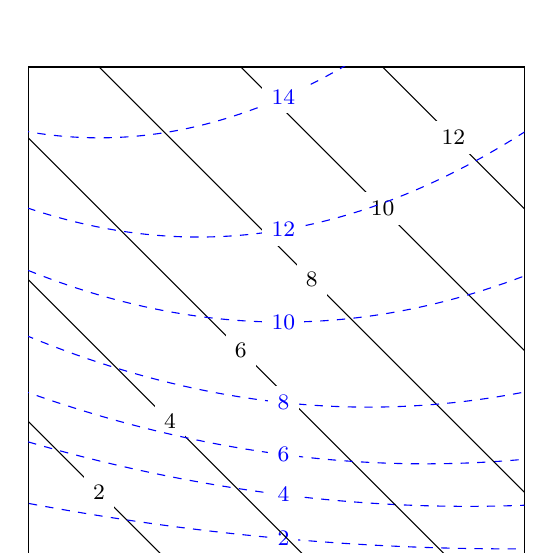
\begin{tikzpicture}[scale=1.8]
  \clip[draw] (0,0) rectangle (3.5, 3.5);

  % Solid lines
  \foreach \xa/\xb/\yb/\xl in {1 / 3.4 / 1   / 2, 
                               2 / 3.1 / 1.7 / 4, 
                               3 / 2.8 / 2.3 / 6, 
                               4 / 2.4 / 3.1 / 8, 
                               5 / 1.8 / 4   / 10, 
                               6 / 1.2 / 5   / 12, 
                               8 / 0.5 / 6   / 14}{

    % Straight lines -- solid and black
    \draw[name path=w] (0,\xa) -- node[midway,fill=white]{$\xl$} 
                       (\xa,0);

    % Parabolas -- dashed and blue
    \draw[dashed, blue, name path=p] (\xb-6,3.5-\xb+\yb) 
      parabola bend (\xb,3.5-\xb) (\xb+6,3.5-\xb+\yb);

    \path[name path=v] (1.8,0) -- (1.8,3.5);
    \path[name intersections={of=v and p}];
    \coordinate (A) at (intersection-1);
    \node[blue, fill=white] at (A) {$\xl$};
  };
\end{tikzpicture}
\end{center}
\end{question}

\begin{solution}
The points are marked in the figure below.
\begin{center}
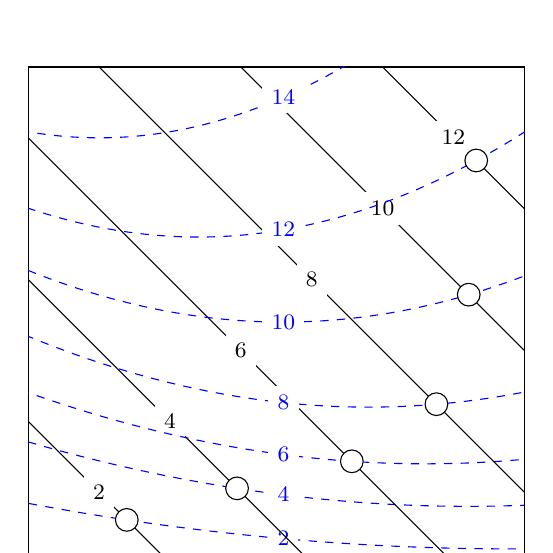
\begin{tikzpicture}[scale=1.8]
  \clip[draw] (0,0) rectangle (3.5, 3.5);

  % Solid lines
  \foreach \xa/\xb/\yb/\xl in {1 / 3.4 / 1   / 2, 
                               2 / 3.1 / 1.7 / 4, 
                               3 / 2.8 / 2.3 / 6, 
                               4 / 2.4 / 3.1 / 8, 
                               5 / 1.8 / 4   / 10, 
                               6 / 1.2 / 5   / 12, 
                               8 / 0.5 / 6   / 14}{

    % Straight lines -- solid and black
    \draw[name path=w] (0,\xa) -- node[midway,fill=white]{$\xl$} 
                       (\xa,0);

    % Parabolas -- dashed and blue
    \draw[dashed, blue, name path=p] (\xb-6,3.5-\xb+\yb) 
      parabola bend (\xb,3.5-\xb) (\xb+6,3.5-\xb+\yb);

    \path[name path=v] (1.8,0) -- (1.8,3.5);
    \path[name intersections={of=v and p}];
    \coordinate (A) at (intersection-1);
    \node[blue, fill=white] at (A) {$\xl$};
    
    % Solution circles
    \path[name intersections={of=w and p}];
    \coordinate (B) at (intersection-1);
    \draw[fill=white] (B) circle (0.08);
  };
\end{tikzpicture}
\end{center}
\end{solution}

\begin{question}
Consider the function $f(x,y) = 3y^2 - 4x^3$. Suppose you are standing on the surface at the point where $x=3$ and $y=-1$. If you start to move on the surface parallel to the $y$-axis in the direction of increasing $y$, does your height increase or decrease?
\end{question}

\begin{solution}
With $x=3$ fixed, our height, when moving parallel to the $y$-axis, will be described by the function
\[
g(y) = f(3,y) = 3y^2 - 108\,.
\]
The graph of $g$ is a parabola, shifted downwards by 108, whose graph is sketched below. Thus, if we increase $y$, starting at $y=-1$, the value of $z$ will decrease.

\begin{center}
\begin{tikzpicture}[scale=0.9375, baseline=0]
 \def\scale{0.9375}

 % \draw[coordinate grid, step=0.5] (-2, -2) grid (2, 2);
 \drawxaxis[$y$]{-2}{2}
 \drawyaxis[$z$]{-2}{2}

 \draw plot[parametric, domain=-2:2, samples=100] function {t, t**2-1.75}
   node[right] {$z = f(3,y)$};

 \coordinate (a) at (-0.5, {0.25-1.75});
 \draw[dashed] (-0.5, 0) -- (a);
 \drawpoint{(a)}

 \drawxlabels{-0.5/-1}

\end{tikzpicture}
\end{center}
\end{solution}

\begin{question}
Determine which surface (1) -- (3) corresponds to which defining equation (a) -- (c).
\begin{tasks}(3)
\task
$x^2 + y^2 = 1$
\task
$x^2 + z^2 = 1$
\task
$y^2 + z^2 = 1$
\end{tasks}

\begin{center}
\begin{tabu} to \linewidth {X[1,c] X[1,c] X[1,c]}
\asyinclude[width=4cm]{asy/match_cylinder_x.asy} &
\asyinclude[width=4cm]{asy/match_cylinder_y.asy} &
\asyinclude[width=3cm]{asy/match_cylinder_z.asy} \\
(1) & 
(2) & 
(3)
\end{tabu}
\end{center}
\end{question}

\begin{solution}
We have the following correspondences:

\begin{center}
\begin{tabu} to \linewidth {X[1,c] X[1,c] X[1,c]}
\asyinclude[width=4cm]{asy/match_cylinder_x.asy} &
\asyinclude[width=4cm]{asy/match_cylinder_y.asy} &
\asyinclude[width=3cm]{asy/match_cylinder_z.asy} \\
(1) -- (c) $y^2 + z^2 = 1$ & 
(2) -- (b) $x^2 + z^2 = 1$ & 
(3) -- (a) $x^2 + y^2 = 1$
\end{tabu}
\end{center}

We can use the method of missing variables to determine them: Note that each of the given equations omits one of the variables $x, y, z$. For example equation (a) omits $z$ and therefore the corresponding surface looks the same, when intersected with any plane $z=c$, where $c \in \R$ is a constant. Only Fig. (3) has this property. 

Similarly, equation (b) omits the variably $y$ and therefore all intersections of its surface with planes $y=c$ looks the same. Only Fig. (2) has this property. Finally, this leaves equation (c), which has to match Fig. (1).
\end{solution}

\begin{question}
Determine which surface (1) -- (3) corresponds to which defining equation (a) -- (c).
\begin{tasks}(3)
\task
$\frac x 4 = y^2 + z^2$
\task
$\frac y 4 = x^2 + z^2$
\task
$\frac z 4 = x^2 + y^2$
\end{tasks}

\begin{center}
\begin{tabu} to \linewidth {X[1,c] X[1,c] X[1,c]}
\asyinclude[width=3.5cm]{asy/match_paraboloid_z.asy} &
\asyinclude[width=3.5cm]{asy/match_paraboloid_x.asy} &
\asyinclude[width=4cm]{asy/match_paraboloid_y.asy} \\
(1) & 
(2) & 
(3)
\end{tabu}
\end{center}
\end{question}

\begin{solution}
We have the following correspondences:

\begin{center}
\begin{tabu} to \linewidth {X[1,c] X[1,c] X[1,c]}
\asyinclude[width=3.5cm]{asy/match_paraboloid_z.asy} &
\asyinclude[width=3.5cm]{asy/match_paraboloid_x.asy} &
\asyinclude[width=4cm]{asy/match_paraboloid_y.asy} \\
(1) -- (c) $\frac z 4 = x^2 + y^2$ & 
(2) -- (a) $\frac x 4 = y^2 + z^2$ & 
(3) -- (b) $\frac y 4 = x^2 + z^2$
\end{tabu}
\end{center}

Note that each of the given equations describes the graph of a function. For example, equation (a) can be regarded as describing the graph of a function $x = f(y,z)$, where $y$ and $z$ are the independent variables and $x$ is the dependent variable. What is the function? In this case $f(y,z) = 4(y^2 + z^2)$. Only Fig. (2) is the graph of a function with $y$, $z$ as independent variables, because only in Fig. (2) is the $x$-coordinate of a point on the surface uniquely determined by the $y$- and $z$-coordinates.

Similarly, equation (b) can be viewed as the graph of a function $y = f(x,z)$ with $x$, $z$ as the independent variables. Only in Fig. (3) can $y$ be viewed as a function of the other variables. Finally, this leaves equation (c), which has to match Fig. (1).
\end{solution}

\begin{question}
Determine which surface (1) -- (3) corresponds to which defining equation (a) -- (c).
\begin{tasks}(3)
\task
$z = y^2-x^2$
\task
$z = 2x^2$
\task
$z = 2y^2$
\end{tasks}

\begin{center}
\begin{tabu} to \linewidth {X[1,c] X[1,c] X[1,c]}
\asyinclude[width=3.5cm]{asy/match_parabola_xz.asy} &
\asyinclude[width=4cm]{asy/match_parabola_xz_2.asy} &
\asyinclude[width=3.5cm]{asy/match_saddle.asy} \\
(1) & 
(2) & 
(3)
\end{tabu}
\end{center}
\end{question}

\begin{solution}
We have the following correspondences:

\begin{center}
\begin{tabu} to \linewidth {X[1,c] X[1,c] X[1,c]}
\asyinclude[width=3.5cm]{asy/match_parabola_xz.asy} &
\asyinclude[width=4cm]{asy/match_parabola_xz_2.asy} &
\asyinclude[width=3.5cm]{asy/match_saddle.asy} \\
(1) -- (b) $z = 2x^2$ & 
(2) -- (c) $z = 2y^2$ & 
(3) -- (a) $z = y^2 - x^2$
\end{tabu}
\end{center}

Only in equation (a) can $z$ -- because of the presence of $-x^2$ -- take negative values. Therefore equation (a) has to correspond to Fig. (3). This leaves equations (b) and (c). To distinguish them we can look at their level sets. For $z=2x^2$, the level sets $z=c$ take the form $2x^2 = c$. They describe the two lines
\[
x = \frac 12 \sqrt{2c} \text{ and } x = -\frac 12 \sqrt{2c}\,.
\]
The level sets in Fig. (1) are lines of the form $x=k$ with some $k \in \R$, while the level sets in Fig. (2) are lines of the form $y=k$. Thus (b) corresponds to (1) and (c) to (2).
\end{solution}

\begin{question}
Match the function with its graph and justify your reasoning.
\begin{tasks}(2)
\task
$f(x,y) = \sin x - \sin y$
\task
$f(x,y) = \sin (x-y)$
\end{tasks}

\begin{center}
\begin{tabu} to \linewidth {X[1,c] X[1,c]}
\asyinclude[width=6.8cm]{asy/match_sin_1.asy} &
\asyinclude[width=6.8cm]{asy/match_sin_2.asy} \\
(1) & 
(2)
\end{tabu}
\end{center}
\end{question}

\begin{solution}
We can distinguish the two functions by looking at the sections $y=k$ for $k \in \R$ a constant.
\begin{enumerate}
\item
For the function $f(x,y) = \sin x - \sin y$ these sections are $z = \sin x - \sin k$. In other words the graph $z = \sin x$ is shifted up and down as $y$ varies.
\item
For the function $f(x,y) = \sin(x-y)$ these sections are $z = \sin (x-k)$. In other words the graph $z = \sin x$ is shifted to the right and to the left as $y$ varies.
\end{enumerate}

So we conclude that the right correspondences are (1) -- (b) and (2) -- (a).
\end{solution}

\begin{question}
Describe the maximal domain of definition for each of the following functions.
\begin{tasks}(2)
\task
$f(x,y) = \displaystyle\frac{y}{x}$
\task
$f(x,y) = \displaystyle\frac{x+y}{x-y}$
\task
$f(x,y) = \displaystyle\frac{x+y}{x^2+y^2-1}$
\task
$f(x,y) = \sqrt{y - x^2}$
\task
$f(x,y) = \sqrt{x} \ln (y-\sin x)$
\task
$f(x,y) = \sqrt{y - \ln(-x)}$
\end{tasks}
\end{question}

\begin{solution}
We will denote by $D(f)$ the maximal domain of definition.
\begin{enumerate}
\item
The function can be defined everywhere, where $x \neq 0$. Therefore
\[
D(f) = \{ (x,y)\,:\, x \neq 0 \} = \R^2 \setminus \{ x = 0 \} \,;
\]
the domain consists of the whole plane except for the $y$-axis.
\item
The function can be defined everywhere, where $x - y \neq 0$. Therefore
\[
D(f) = \{ (x,y) \,:\, x \neq y \} = \R^2 \setminus \{ x=y \} \,;
\]
the domain consists of the whole plane except for those points lying on the line $x=y$.
\item
Here the denominator is $0$, when $x^2 + y^2 = 1$. Therefore
\[
D(f) = \{ (x,y) \,:\, x^2 + y^2 \neq 1 \} = \R^2 \setminus \{ x^2 + y^2 = 1\} \,;
\]
the domain conists of the whole plane except for the circle around the origin with radius 1.
\end{enumerate}

\begin{center}
\begin{figuretable}{3}
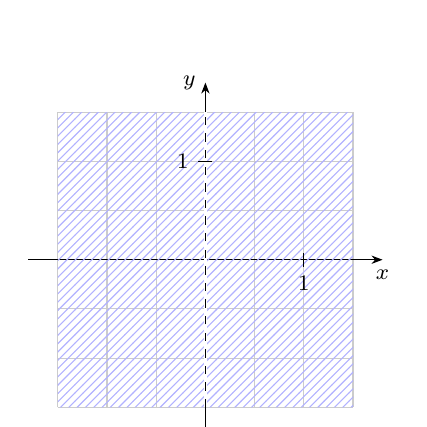
\begin{tikzpicture}[scale=1.25, baseline=0]
 \def\scale{1.25}

 \draw[coordinate grid, step=0.5] (-1.5, -1.5) grid (1.5, 1.5);
 \drawaxes{-1.5}{-1.5}{1.5}{1.5}

 \fill[pattern color=blue!30, pattern=north east lines] (-1.5, -1.5) |- (1.5, 1.5) |- cycle;
 \draw[draw=white, very thick] (0, -1.5) -- (0, 1.5);
 \draw[draw=black, dashed] (0, -1.5) -- (0, 1.5);

 \drawxlabels[nofill]{1/1}
 \drawylabels[nofill]{1/1}
\end{tikzpicture}
&
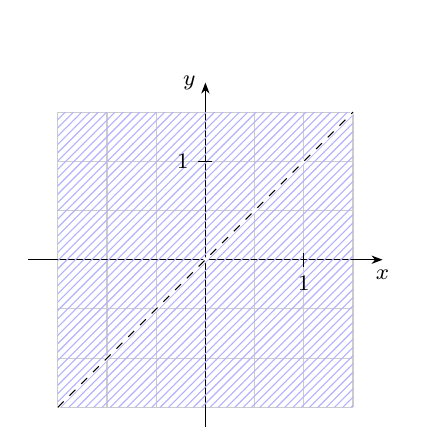
\begin{tikzpicture}[scale=1.25, baseline=0]
 \def\scale{1.25}

 \draw[coordinate grid, step=0.5] (-1.5, -1.5) grid (1.5, 1.5);
 \drawaxes{-1.5}{-1.5}{1.5}{1.5}

 \fill[pattern color=blue!30, pattern=north east lines] (-1.5, -1.5) |- (1.5, 1.5) |- cycle;
 \draw[draw=white, very thick] (-1.5, -1.5) -- (1.5,1.5);
 \draw[draw=black, dashed] (-1.5,-1.5) -- (1.5, 1.5);

 \drawxlabels[nofill]{1/1}
 \drawylabels[nofill]{1/1}
\end{tikzpicture}
&
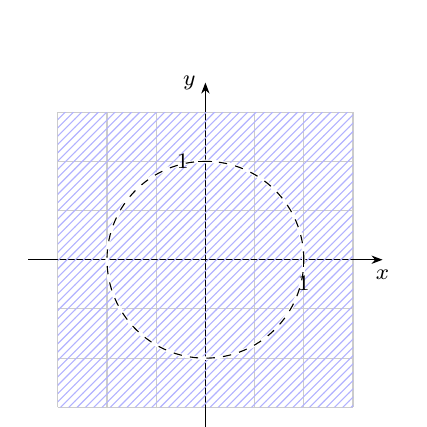
\begin{tikzpicture}[scale=1.25, baseline=0]
 \def\scale{1.25}

 \draw[coordinate grid, step=0.5] (-1.5, -1.5) grid (1.5, 1.5);
 \drawaxes{-1.5}{-1.5}{1.5}{1.5}

 \fill[pattern color=blue!30, pattern=north east lines] (-1.5, -1.5) |- (1.5, 1.5) |- cycle;
 \draw[draw=white, very thick] (0,0) circle [radius=1];
 \draw[draw=black, dashed] (0,0) circle [radius=1];

 \drawxlabels[nofill]{1/1}
 \drawylabels[nofill]{1/1}
\end{tikzpicture} \\
(a) & (b) & (c)
\end{figuretable}
\end{center}

\begin{enumerate}[resume]
\item
For the square root to be well-defined we need the inequality $y - x^2 \geq 0$ to be satisfied. Therefore
\[
D(f) = \{ (x,y) \,:\, y \geq x^2 \}\,;
\]
the domain consists of the part of the plane, that lies on and above the parabola $y=x^2$.
\item
Here we need $x \geq 0$ for the square root to be well-defined and $y > \sin x$ to evaluate the logarithm. Note that one inequality is strict, while the other is not. Thus the domain is
\[
D(f) = \{ (x,y)\,:\, x \geq 0 \text{ and } y > \sin x \}\,;
\]
\item
To be able to evaluate $f(x,y)$ we need $-x > 0$ as well as $y - \ln(-x) \geq 0$ to be satisfied. These inequalities can be rewritten as
\[
D(f) = \{ (x,y) \,:\, x < 0 \text{ and } y \geq \ln(-x) \}\,.
\]
Note again, that one inequality is strict and the other is not.
\end{enumerate}

\begin{center}
\begin{figuretable}{3}
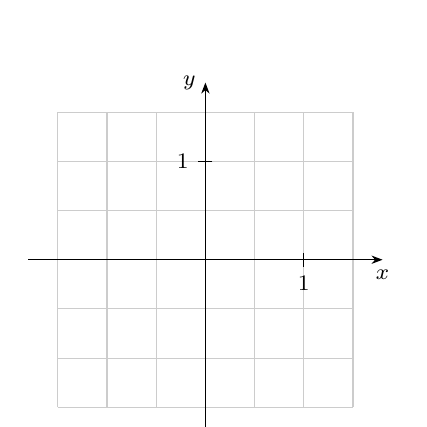
\begin{tikzpicture}[scale=1.25, baseline=(X.base)]
  \def\scale{1.25}
  \draw[coordinate grid, step=0.5] (-1.5,-1.5) grid (1.5,1.5);
  \node at (0,-1.5) (X) {};

  \drawaxes{-1.5}{-1.5}{1.5}{1.5}

  \clip (-1.5, -1.5) rectangle (1.5, 1.5);

  \fill[pattern color=blue!30, pattern=north east lines]
    plot[parametric, domain=-1.5:1.5, samples=100] function {t, t**2}
    -- cycle;

  \draw plot[parametric, domain=-1.5:1.5, samples=100] function {t, t**2};

  \drawxlabels[nofill]{1/1}
  \drawylabels[nofill]{1/1}
\end{tikzpicture}
&
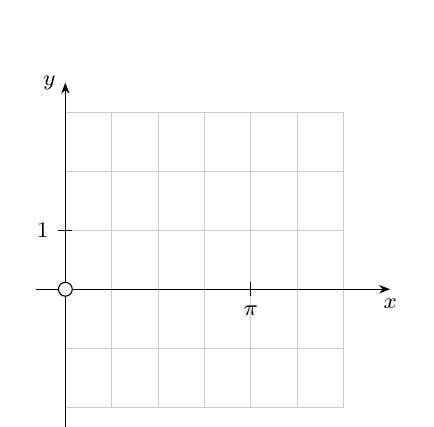
\begin{tikzpicture}[scale=0.75, baseline=(X.base)]
 \def\scale{0.75}

 \draw[coordinate grid, xstep={pi/4}] (0, -2) grid ({3*pi/2}, 3);
 \node at (0,-2) (X) {};
 \drawaxes{0}{-2}{5}{3}

 \fill[pattern color=blue!30, pattern=north east lines]
   plot[domain={0:3*pi/2}, samples=100] function {sin(x)}
   |- (0, 3) -- cycle;

 \draw[draw=white, very thick] 
   plot[domain={0:3*pi/2}, samples=100] function {sin(x)};
 \draw[draw=black, dashed, domain={0:3*pi/2}, samples=100]
      plot[parametric] function {t, sin(t)};

 \drawpoint{(0,0)}

 \drawxlabels[]{pi/{\pi}}
 \drawylabels[]{1/1}
\end{tikzpicture}
&
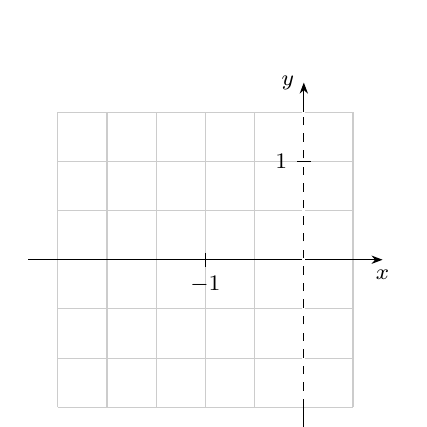
\begin{tikzpicture}[scale=1.25, baseline=(X.base)]
 \def\scale{1.25}

 \draw[coordinate grid, step=0.5] (-2.5, -1.5) grid (0.5, 1.5);
 \drawaxes{-2.5}{-1.5}{0.5}{1.5}
 \node at (0,-1.5) (X) {};

 \draw[draw=white, very thick] (0,-1.5) -- (0,1.5);
 \draw[draw=black, dashed] (0,-1.5) -- (0,1.5);

 \clip (-2.5, -1.5) rectangle (0.5, 1.5);

 \draw plot[domain=-0.001:-3, samples=100] function {log(-x)};

 \fill[pattern color=blue!30, pattern=north east lines] 
    plot[domain=-3:-0.001, samples=100] function {log(-x)}
    -| (0,1.5) -| cycle;


 \drawxlabels[nofill]{-1/-1}
 \drawylabels[nofill]{1/1}
\end{tikzpicture}
\\
(d) & (e) & (f)
\end{figuretable}
\end{center}
\end{solution}

\begin{question}
Sketch the graphs of the following functions
\begin{tasks}(2)
\task
$f(x,y) = 2-x-y$
\task
$z=x+2$
\end{tasks}
\end{question}

\begin{solution}
\begin{enumerate}
\item
The graph consists of all points satisfying the equation
\[
z=2-x-y\,.
\]
This is the equation of a plane. To visualize it we can calculate, where the plane intersects the coordinate axes:
\begin{itemize}
\item
$x$-axis at $(2,0,0)$;
\item
$y$-axis at $(0,2,0)$;
\item
$z$-axis at $(0,0,2)$.
\end{itemize}

\item
The graph of this function is again a plane. Furthermore, the equation of the graph
\[
z = x+2
\]
does not contain the variable $y$ and hence we can draw the line $z=x+2$ in the $yz$-plane and then prolong it along the $y$-direction.
\end{enumerate}

\begin{center}
\begin{tabu} to \linewidth {X[1,c] X[1,c]}
\asyinclude[width=4cm]{asy/graph_plane_111.asy} &
\asyinclude[width=5cm]{asy/graph_plane_xp2.asy} \\
(a) & (b)
\end{tabu}
\end{center}
\end{solution}

\begin{question}
Sketch the level curves for the following functions and the values $-2, -1, 1, 2$ and describe the level curve for a general value $c \in \R$.
\begin{tasks}(3)
\task
$f(x,y) = \frac{y}{x}$
\task
$f(x,y) = \frac{x+y}{x-y}$
\task
$f(x,y) = \frac{x+y}{x^2+y^2-1}$
\end{tasks}
{\itshape Hint:} When determining the level curves in (c), complete the squares in the expression instead of solving for $x$ or $y$.
\end{question}

\begin{solution}
We will discuss directly the general case. The level curves for the specific values can be found in the figures below.
\begin{enumerate}
\item
The level curve for the value $c$ consists of all points that solve the equation
\[
\frac y x = c\,.
\]
This equation is equivalent to
\[
y = cx\,.
\]
These are lines through the origin with slope $c$. Note that the point $(0,0)$ lies on the line $y=cx$, but is not part of the level set, since $(0,0)$ does not lie in the domain of definition of $f$.

Note that as $c$ approaches $+\infty$ or $-\infty$, the lines $y=cx$ approach the $y$-axis, where the function is not defined.

\item
The level curve for the value $c$ consists of all points that solve the equation
\[
x+y = c(x-y)\,.
\]
When $c \neq -1$ we can solve the equation for $y$ and obtain
\[
y= \frac{c-1}{c+1} x\,.
\]
Thus the level curves are lines through the origin with different slopes. As in (a), the point $(0,0)$ is not part of the level set, because it does not lie in the domain of definition of $f$.

For $c=-1$ the level curve is given by the equation
\[
x+y = -(x-y)\,,
\]
which is equivalent to
\[
x=0\,.
\]
Again, the point $(0,0)$ is not part of the level set.

What happens when $c$ approached $+\infty$? A simple calculation shows that
\[
\lim_{c \to +\infty} \frac{c-1}{c+1} = 1\,,
\]
and thus the level curves approach the line $x=y$, where $f$ is not defined.

\item
The level curve for the value $c$ consists of all points that are solutions to the equation
\[
x + y = c\left( x^2 + y^2 - 1\right)\,.
\]
When $c \neq 0$, this equation can, by completing the squares, be rewritten as
\[
\left(x - \frac 12 c\inv\right)^2 + \left(y - \frac 12 c\inv\right)^2 = 1 + \frac 12 c^{-2}\,,
\]
and it describes a circle with center $\left(\frac 12 c\inv, \frac 12 c\inv\right)$ and radius $\sqrt{1 +  \frac 12 c^{-2}}$.

Note that two points on the circle are not part of the level set: these are the points, where the level set circle intersects the circle $x^2 + y^2 = 1$, since at these points the function is not defined.

Not all level sets are circles. When $c=0$, the equation for level sets simplifies to
\[
x+y = 0\,.
\]
Therefore the $0$-level set is the line through the origin with slope $1$.
\end{enumerate}

\begin{center}
\begin{figuretable}{3}
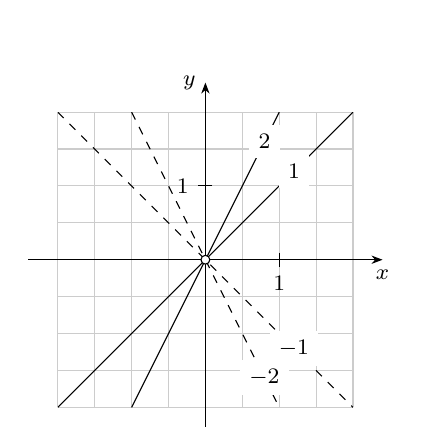
\begin{tikzpicture}[scale=0.9375, baseline=(X.base)]
  \def\scale{0.9375}
  \draw[coordinate grid, step=0.5] (-2,-2) grid (2, 2);
  \node at (0,0) (X) {};

  \drawaxes{-2}{-2}{2}{2}

  \clip (-2, -2) rectangle (2, 2);

  \draw[dashed] (-1, 2) -- (1, -2) node[fill=white, pos=0.9]{$-2$};
  \draw[dashed] (-2, 2) -- (2, -2) node[fill=white, pos=0.8]{$-1$};

  \draw (-1, -2) -- (1, 2) node[fill=white, pos=0.9]{$2$};
  \draw (-2, -2) -- (2, 2) node[fill=white, pos=0.8]{$1$};
  \draw[draw=black, fill=white] (0,0) circle [radius=0.06];

  \drawxlabels[nofill]{1/1}
  \drawylabels[nofill]{1/1}
\end{tikzpicture}
&
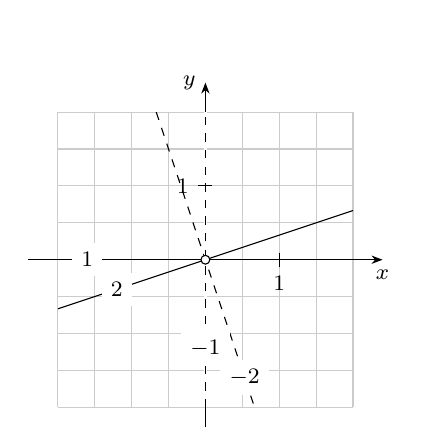
\begin{tikzpicture}[scale=0.9375, baseline=(X.base)]
  \def\scale{0.9375}
  \draw[coordinate grid, step=0.5] (-2,-2) grid (2, 2);
  \node at (0,0) (X) {};

  \drawaxes{-2}{-2}{2}{2}

  \clip (-2, -2) rectangle (2, 2);

  \draw[dashed] (-0.666, 2) -- (0.666, -2) node[fill=white, pos=0.9]{$-2$};
  \draw[draw=white, very thick] (0,-2) -- (0,2);
  \draw[dashed] (0, -2) -- (0, 2) node[fill=white, pos=0.2]{$-1$};

  \draw (-2, 0) -- (2, 0) node[fill=white, pos=0.1]{$1$};
  \draw (-2, -0.666) -- (2, 0.666) node[fill=white, pos=0.2]{$2$};
  \draw[draw=black, fill=white] (0,0) circle [radius=0.06];

  \drawxlabels[nofill]{1/1}
  \drawylabels[nofill]{1/1}
\end{tikzpicture}
&
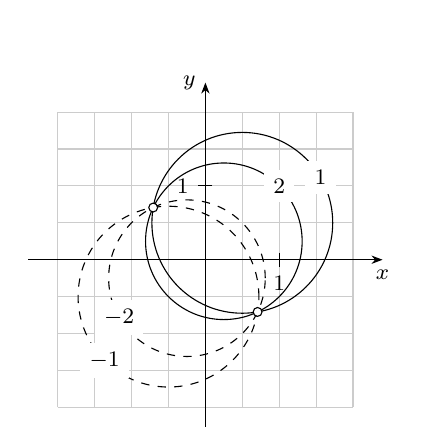
\begin{tikzpicture}[scale=0.9375, baseline=(X.base)]
  \def\scale{0.9375}
  \draw[coordinate grid, step=0.5] (-2,-2) grid (2, 2);
  \node at (0,0) (X) {};

  \drawaxes{-2}{-2}{2}{2}

  \clip (-2, -2) rectangle (2, 2);

  \draw[dashed] (-0.25, -0.25) circle [radius={3/sqrt(8)}];
  \node[fill=white] at ($(-0.25,-0.25)+(210:{3/sqrt(8)})$) {$-2$};

  \draw[dashed] (-0.5, -0.5) circle [radius={sqrt(6)/2)}];
  \node[fill=white] at ($(-0.5,-0.5)+(225:{sqrt(6)/2})$) {$-1$};

  \draw (0.5, 0.5) circle [radius={sqrt(6)/2)}];
  \node[fill=white] at ($(0.5,0.5)+(30:{sqrt(6)/2})$) {$1$};

  \draw (0.25, 0.25) circle [radius={3/sqrt(8)}];
  \node[fill=white] at ($(0.25,0.25)+(45:{3/sqrt(8)})$) {$2$};

  \draw[draw=black, fill=white] (135:1) circle [radius=0.06];
  \draw[draw=black, fill=white] (-45:1) circle [radius=0.06];

  \drawxlabels[nofill]{1/1}
  \drawylabels[nofill]{1/1}
\end{tikzpicture}
\\
(a) & (b) & (c)
\end{figuretable}
\end{center}
\end{solution}

% \begin{question}
% Sketch the surface in space defined by each of the following equations
% \begin{enumerate}
% \item
% $z=x^2+2$
% \item
% $z=|y|$
% \item
% $z^2+x^2=4$
% \item
% $z=(x-1)^2 + y^2$
% \item[(e*)]
% $z=\max(|x|,|y|)$ \\
% {\itshape Note:} $\max(|x|, |y|)$ is the maximum of $|x|$ and $|y|$.
% \end{enumerate}
% \end{question}

% \begin{solution}
% \begin{enumerate}
% \item
% The function 
% \[
% f(x,y) = x^2 + 2
% \]
% does not depend on $y$ and hence we can draw the parabola $z=x^2$ in the $xz$-plane and then extend it along the $y$-direction.
% \item
% The function
% \[
% f(x,y) = |y|
% \]
% does not depend on $x$. We can thus draw the function $z=|y|$ in the $yz$-plane and then extend it along the $x$-direction.
% \item
% The equation
% \[
% z^2 + x^2 = 4
% \]
% does not depend on $y$ and describes a circle of radius 2 in the $xz$-plane. Hence the surface in $xyz$-space is a cylinder along the $y$-axis.
% \item
% To understand the graph of the function
% \[
% f(x,y) = (x-1)^2 + y^2
% \]
% we look at level sets for a value $c$. These are given by the equation
% \[
% (x-1)^2 + y^2 = c\,.
% \]
% We see that level sets are circles around the point $(1,0)$ with radius $\sqrt{c}$.
% \item
% For the function
% \[
% f(x,y) = \max (|x|, |y|)
% \]
% we also look at the level sets. The level set with value $c$ is the square with side length $2c$, centered around the origin, whose edges are parallel to the coordinate axes.
% \end{enumerate}

% \begin{figure}[h]
% \begin{center}
% \includegraphics[width=.44\textwidth]{figures/problems1_4a.png}
% \includegraphics[width=.44\textwidth]{figures/problems1_4b.png} 
% \vspace{.3cm} \\
% \includegraphics[width=.44\textwidth]{figures/problems1_4c.png}
% \includegraphics[width=.44\textwidth]{figures/problems1_4d.png} 
% \vspace{.3cm} \\
% \includegraphics[width=.44\textwidth]{figures/problems1_4e.png}
% \end{center}
% \caption{Graphs of the surfaces in 4(a)-(e).}
% \end{figure}
% \end{solution}

%%% Local Variables:
%%% mode: latex
%%% TeX-master: "problems"
%%% End:

\ifthenelse{\boolean{sectionnewpage}}{\newpage}{}
% Version: v2

\section{Introduction to Partial Derivatives}
\begin{question}
How is the partial derivative $\frac{\p g}{\p v}$ of the function $g(u, v, w)$ defined?
\end{question}

\begin{solution}
The partial derivative is defined as the limit
\[
\frac{\p g}{\p v}(u, v, w) = \lim_{h \to 0} \frac{g(u, v + h, w) - g(u, v, w)}{h}\,.
\]
\end{solution}

\begin{question}
Which of the following show correct notation for the partial derivative of a function $f(x,y)$?
\begin{tasks}(4)
\task
$f_x(x,y)$
\task
$\frac{df}{dx}(x,y)$
\task
$\frac{\p f}{\p x}(x,y)$
\task
$f'(x)$
\end{tasks}
\end{question}

\begin{solution}
(a) and (c).

The notation $\frac{d f}{dx}$ is reserved for derivatives of functions, that depend only on one variable. For functions of several variables we replace $d$ by $\p$ and write $\frac{\p f}{\p x}$ instead.

The notation $f'(x)$ is also used only for functions of one variable. By itself $f'$ does not show, which partial derivative is mean ($f_x$ or $f_y$). Writing $f'(x)$ is wrong, because $f$ and its partial derivatives are functions of both $x$ and $y$.
\end{solution}

\begin{question}
\SetQuestionProperties{source = {Ex. 1--5; MW, III.15.1}}
Compute $f_x$ and $f_y$ for the following functions and evaluate them at the indicated points.
\begin{tasks}(2)
\task
$f(x,y) = xy + x -y;\, (1,1)$
\task
$f(x,y) = x/y;\, (1,1)$
\task
$f(x,y) = \arctan(x-3y^2);\, (1,0)$
\task
$f(x,y) = x + \sqrt{x^2+y^2};\, (1,-1)$
\task
$f(x,y) = e^{xy}\sin(x+y);\, (0,0)$
\task
$f(x,y) = x^y;\, (e,2)$
% \task
% $f(x,y) = \ln(x^2+y^2+1);\, (0,0)$
\end{tasks}
\end{question}

\begin{solution}
\begin{enumerate}
\item
We have
\begin{align*}
f_x(x,y) &= y +1 &
f_y(x,y) &= x-1\,,
\end{align*}
and so $f_x(1,1) = 2$ and $f_y(1,1) = 0$.
\item
We have
\begin{align*}
f_x(x,y) &= \frac{1}{y} &
f_y(x,y) &= -\frac{x}{y^2}\,,
\end{align*}
and so $f_x(1,1) = 1$ and $f_y(1,1) = -1$.
\item
We have
\begin{align*}
f_x(x,y) &= \frac{1}{1+\left(x-3y^2\right)^2} &
f_y(x,y) &= \frac{-6y}{1+\left(x-3y^2\right)^2}\,,
\end{align*}
and so $f_x(1,0) = \frac 12$ and $f_y(1,0) = 0$.
\item
We have
\begin{align*}
f_x(x,y) &= 1 + \frac{x}{\sqrt{x^2+y^2}} &
f_y(x,y) &= \frac{y}{\sqrt{x^2+y^2}} \,,
\end{align*}
and so $f_x(1,-1) = 1 + \frac{\sqrt{2}}{2}$ and $f_y(1,-1) = -\frac{\sqrt{2}}2$.
\item
We have
\begin{align*}
f_x(x,y) &= y e^{xy} \sin(x+y) + e^{xy} \cos(x+y) \\
f_y(x,y) &= x e^{xy} \sin(x+y) + e^{xy} \cos(x+y)\,,
\end{align*}
and so $f_x(0,0) = 1$ and $f_y(0,0) = 1$.
\item
To compute the $y$-derivative we write $f(x,y) = x^y = e^{y \ln x}$. We have
\begin{align*}
f_x(x,y) &= y x^{y-1} &
f_y(x,y) &= x^y \ln x\,,
\end{align*}
and so $f_x(e, 2) = 2e$ and $f_y(e, 2) = e^2$.
% \item
% We have
% \begin{align*}
% f_x(x,y) &= \frac{2x}{x^2 + y^2 + 1} \\
% f_y(x,y) &= \frac{2y}{x^2 + y^2 + 1} \,,
% \end{align*}
% and so $f_x(0,0) = 0$ and $f_y(0,0) = 0$.
\end{enumerate}
\end{solution}

\begin{question}
\SetQuestionProperties{source = {Ex. 21, 22, 37--40; MW, III.15.1}}
Compute the indicated partial derivatives.
\begin{tasks}(2)
\task
$\frac{\p}{\p y}\left( \frac{x e^y - 1}{y e^x + 1}\right)$
\task
$\frac{\p}{\p u} \big( uvw - \sin(uvw) \big)$
\task
$\frac{\p}{\p s} e^{stu^2}$
\task
$\frac{\p}{\p r} \left( \frac 13 \pi r^2 h \right)$ 
\task
$\frac{\p}{\p \la} \left( \frac{\cos \la\mu}{1+\la^2 + \mu^2} \right)$
\task
$\frac{\p}{\p a} \left( bcd \right)$
\end{tasks}
\end{question}

\begin{solution}
\begin{enumerate}
\item
\begin{align*}
\frac{\p}{\p y}\left( \frac{x e^y - 1}{y e^x + 1} \right)
&= \frac{xe^y \left(y e^x + 1\right) - \left(xe^y - 1\right) e^x}
{\left( ye^x + 1\right)^2}
= \frac{xy e^{x+y}  - x e^{x+y} + xe^y + e^x}
{\left( ye^x + 1\right)^2}\,.
\end{align*}
\item
\begin{align*}
\frac{\p}{\p u} \left( uvw - \sin(uvw) \right)
&= vw - vw \cos(uvw) = vw( 1 - \cos(uvw))\,.
\end{align*}
\item
\[
\frac{\p}{\p s} e^{stu^2} = tu^2 e^{stu^2}\,.
\]
\item
\[
\frac{\p}{\p r}\left(\frac 13 \pi r^2 h\right) = \frac 23 \pi r h\,.
\]
\item
\begin{align*}
\frac{\p}{\p \la} \left( \frac{\cos \la\mu}{1+\la^2 + \mu^2} \right)
&= \frac{ - \mu \sin (\la \mu) \left( 1+ \la^2+\mu^2\right)
- 2\la \cos(\la \mu)}
{\left(1+\la^2+\mu^2\right)^2} \\
&=  -\frac{\mu \sin \la \mu}
{1+\la^2+\mu^2} - \frac{2\la \cos \la\mu}{\left(1+\la^2+\mu^2\right)^2}\,.
\end{align*}
\item
\[
\frac{\p}{\p a} \left( bcd \right) = 0\,,
\]
because the function $bcd$ does not depend on the variable $a$.
\end{enumerate}
\end{solution}

\begin{question}
\SetQuestionProperties{source = {Ex. 45; MW, III.15.1}}
If three resistors $R_1$, $R_2$ and $R_3$ are connected in parallel, the total electrical resistance is determined by the equation
\[
\frac{1}{R} = \frac{1}{R_1} + \frac{1}{R_2} + \frac{1}{R_3}\,.
\]
\begin{enumerate}
\item
What is $\p R/\p R_1$?
\item
Suppose that $R_1$, $R_2$ and $R_3$ are variable resistors set at 100, 200 and 300 ohms respectively. How fast is $R$ changing with respect to $R_1$?
\end{enumerate}
\end{question}

\begin{solution}
First we express $R$ as a function of $R_1$, $R_2$ and $R_3$,
\[
R = \frac{1}{R_1\inv + R_2\inv + R_3\inv}\,,
\]
and then we differentiate
\[
\frac{\p R}{\p R_1} = \frac{R_1^{-2}}{\left(R_1\inv + R_2\inv + R_3\inv\right)^2} \,.
\]
To simplify the expression note that
\[
\frac{1}{R_1} + \frac{1}{R_2} + \frac{1}{R_3} = \frac{R_1R_2 + R_1R_3 + R_2 R_3}{R_1R_2 R_3}\,.
\]
Thus
\[
\frac{\p R}{\p R_1} = \frac{1}{R_1^2} \frac{R_1^2R_2^2 R_3^2}{\left(R_1R_2 + R_1R_3 + R_2 R_3\right)^2}
= \frac{R_2^2 R_3^2}{\left(R_1R_2 + R_1R_3 + R_2 R_3\right)^2}\,.
\]

If $R_1$, $R_2$ and $R_3$ are set at 100, 200 and 300 ohms, then
\[
\frac{\p R}{\p R_1}(100,200,300) = \frac{36}{121}\,.
\]
\end{solution}

\begin{question}
Consider the contour plot for the function $f(x,y)$. Determine whether the following quantities are \emph{positive}, \emph{negative} or \emph{zero}.

\begin{center}
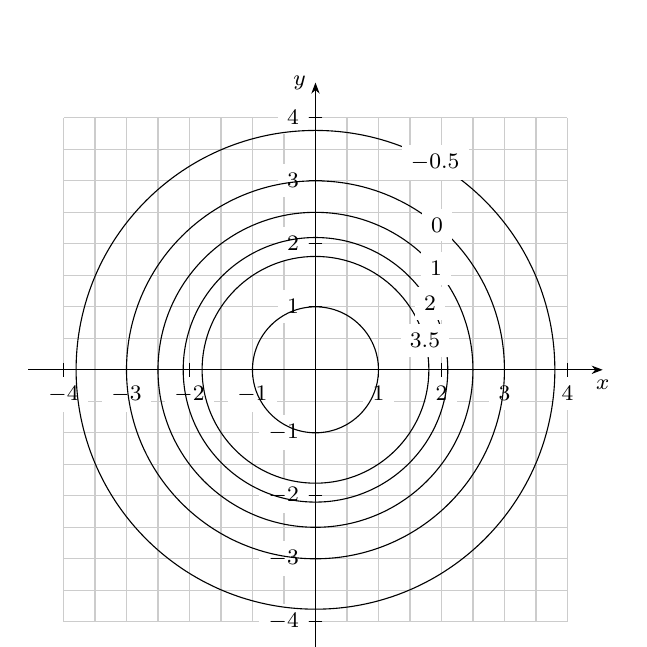
\begin{tikzpicture}[scale=0.8, baseline=0]
  \def\scale{0.8}
  \draw[coordinate grid, step=0.5] (-4,-4) grid (4,4);

  \drawxlabels{-4/-4, -3/-3, -2/-2, -1/-1, 1/1, 2/2, 3/3, 4/4}
  \drawylabels{-4/-4, -3/-3, -2/-2, -1/-1, 1/1, 2/2, 3/3, 4/4}
  \drawaxes{-3.8}{-3.8}{3.8}{3.8}

  \draw[name path=c1] (0,0) circle (1.);
  \draw[name path=c2] (0,0) circle (1.8);
  \draw[name path=c2] (0,0) circle (2.1);
  \draw[name path=c3] (0,0) circle (2.5);
  \draw[name path=c4] (0,0) circle (3);
  \draw[name path=c5] (0,0) circle (3.8);

  \node[fill=white] at (15:1.8) {$3.5$};
  \node[fill=white] at (30:2.1) {$2$};
  \node[fill=white] at (40:2.5) {$1$};
  \node[fill=white] at (50:3) {$0$};
  \node[fill=white] at (60:3.8) {$-0.5$};
\end{tikzpicture}
\end{center}

\begin{tasks}(3)
\task
$\frac{\p f}{\p x}(2,-1.5)$
\task
$\frac{\p^2 f}{\p x^2}(2,-1.5)$
\task
$\frac{\p f}{\p y}(3,0)$
\end{tasks}
\end{question}

\begin{solution}
\begin{enumerate}
\item
We can read off the contour plot that
\begin{align*}
f(1.5, -1.5) &= 2 &
f(2,-1.5) &= 1 &
f(2.5, 1.5) &\approx 0\,.
\end{align*}
In particular $f(x,-1.5)$ is decreasing around $x=2$. Therefore $\frac{\p f}{\p x}(2,-1.5) < 0$.

\item
From the figure we see that the function $f(x,-1.5)$ is convex around $x=2$. Therefore $\frac{\p^2 f}{\p x^2}(2,-1.5) > 0$.

\begin{center}
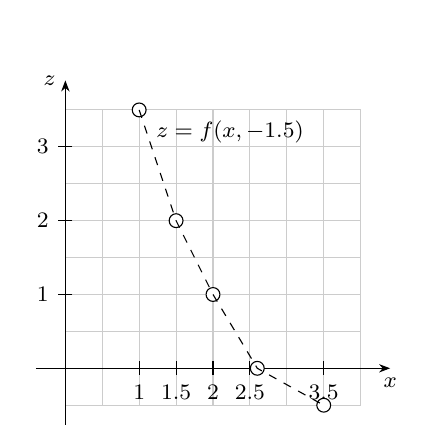
\begin{tikzpicture}[scale=0.9375, baseline=0]
 \def\scale{0.9375}

 \draw[coordinate grid, step=0.5] (0, -0.5) grid (4, 3.5);
 \drawaxeslabelled{0}{-0.5}{4}{3.5}{$x$}{$z$}

 \drawpoint{(1,3.5)};
 \drawpoint{(1.5,2)};
 \drawpoint{(2,1)};
 \drawpoint{(2.6,0)};
 \drawpoint{(3.5,-0.5)};

 \draw[dashed] (1,3.5) -- node[pos=0.2, right] {$z = f(x,-1.5)$} (1.5,2) -- (2,1)
   -- (2.6,0) -- (3.5,-0.5);

 \drawxlabels[nofill]{1/1, 1.5/1.5, 2/2, 2.5/2.5, 3.5/3.5}
 \drawylabels[nofill]{1/1, 2/2, 3/3}
\end{tikzpicture}
\end{center}

\item
We can see that $f(3,0) = 0$ and that $y=0$ is a local maximum for the function $f(3,y)$. In particular this implies that $\frac{\p f}{\p y}(3,0) = 0$.
\end{enumerate}
\end{solution}

\begin{question}
\SetQuestionProperties{source = {Ex. 54,55; MW, III.15.1}}
Compute the derivatives 
$\displaystyle\frac{\p^2 u}{\p x^2}$, 
$\displaystyle\frac{\p^2 u}{\p y \p x}$, 
$\displaystyle\frac{\p^2 u}{\p y^2}$ and 
$\displaystyle\frac{\p^2 u}{\p x \p y}$ for the following functions and check directly the equality of the mixed partial derivatives.
\begin{tasks}(2)
% \task
% $\displaystyle
% u = \frac{2xy}{(x^2+y^2)^2}
% $
\task
$u = \cos(xy^2)$
\task
$u = e^{-xy^2} + y^3x^4$
\end{tasks}
\end{question}

\begin{solution}
\begin{enumerate}
% \item
% The function is $\displaystyle
% u = \frac{2xy}{(x^2+y^2)^2}
% $.
% We have
% \begin{align*}
% u_x &= \frac{2y}{(x^2+y^2)^2} - \frac{8x^2 y}{(x^2+y^2)^3}
% = \frac{ -6x^2 y + 2y^3}{(x^2+y^2)^3} \\
% u_y &= \frac{2x}{(x^2+y^2)^2} - \frac{8x y^2}{(x^2+y^2)^3}
% = \frac{2x^3 -6x y^2}{(x^2+y^2)^3} \\
% \end{align*}
% and so
% \begin{align*}
% u_{xx} &= \frac{24xy(x^2-y^2)}{(x^2+y^2)^4} &
% u_{yx} &= \frac{-6(x^4 - 6x^2y^2 + y^4)}{(x^2+y^2)^4} \\
% u_{xy} &= \frac{-6(x^4 - 6x^2y^2 + y^4)}{(x^2+y^2)^4} &
% u_{yy} &= \frac{-24xy(x^2-y^2)}{(x^2+y^2)^4}\,.
% \end{align*}
\item
The function is $u = \cos(xy^2)$.
We have
\begin{align*}
u_x &= -y^2 \sin(xy^2) &
u_y &= -2xy \sin(xy^2)\,,
\end{align*}
and so
\begin{align*}
u_{xx} &= -y^4 \cos(xy^2) &
u_{yx} &= -2y \sin(xy^2) - 2xy^3 \cos(xy^2) \\
u_{xy} &= -2y \sin(xy^2) - 2xy^3 \cos(xy^2) &
u_{yy} &= -2x \sin(xy^2) - 4x^2y^2 \cos(xy^2)\,.
\end{align*}
\item
The function is $u = e^{-xy^2} + y^3x^4$. We have
\begin{align*}
u_{x} &= -y^2 e^{-xy^2} + 4y^3x^3 &
u_{y} &= -2xy e^{-xy^2} + 3y^2x^4\,,
\end{align*}
and so
\begin{align*}
u_{xx} &= y^4 e^{-xy^2} + 12 y^3x^2 &
u_{yx} &= (-2y + 2xy^3) e^{-xy^2} + 12y^2x^3 \\
u_{xy} &= (-2y + 2xy^3) e^{-xy^2} + 12y^2x^3 &
u_{yy} &= (-2x + 4x^2y^2)e^{-xy^2} + 6yx^4\,.
\end{align*}
\end{enumerate}
\end{solution}

\begin{question}
Let $g(u, v, w)$ be a function with continuous third partial derivatives. Which of the following partial derivatives are equal?
\begin{tasks}(4)
\task
$\frac{\p^3 g}{\p u \p v \p w}$
\task
$\frac{\p^3 g}{\p v \p v \p w}$
\task
$\frac{\p^3 g}{\p v \p u \p w}$
\task
$\frac{\p^3 g}{\p w \p u \p u}$
\task
$\frac{\p^3 g}{\p w \p v \p u}$
\task
$\frac{\p^3 g}{\p w \p u \p v}$
\task
$\frac{\p^3 g}{\p v \p w \p v}$
\task
$\frac{\p^3 g}{\p u \p u \p u}$
\end{tasks}
\end{question}

\begin{solution}
The derivatives (a), (c), (e) and (f) are all equal; so are (b) and (g).

As a practical rule, it does not matter in what order we apply partial derivatives, provided the derivatives exist and are continuous.

To give a rigorous argument, why (a), (c), (e) and (f) coincide, we can argue as follows: First we apply the equality of mixed partial derivatives to the function $g_w$, leading to
$\frac{\p^2}{\p u \p v} g_w = \frac{\p^2}{\p v \p u} g_w$. This shows the equality of (a) and (c). Next, we know that $g_{vu} = g_{uv}$ and therefore their $w$-derivatives are also equal, $\frac{\p}{\p w} g_{vu} = \frac{\p}{\p w} g_{uv}$, showing that (e) and (f) coincide. Finally, to show that (c) equals (e) we need to proceed in two steps as follows:
\[
\frac{\p}{\p v} g_{uw} = \frac{\p}{\p v} g_{wu}
= \frac{\p^2}{\p v \p w} g_{u} = \frac{\p^2}{\p w \p v} g_{u}\,.
\]
This concludes the proof.
\end{solution}

\begin{question}
Let
\[
g(u, v, w) = \frac{e^{u^4 + v}}{ 1+ u^2} \sin\left(u + 3v \right) + u^2 \cos \frac w2\,.
\]
Compute the following partial derivatives in the most efficient way.
\begin{tasks}(2)
\task
$g_{uw}$
\task
$g_{vuu} - g_{uuv}$
\end{tasks}
\end{question}

\begin{solution}
\begin{enumerate}
\item
The function $g$ is the sum of two terms and we can observe that the first term does not depend on $w$ at all. It will therefore disappear, when we take the $w$-derivative. Thus we compute
\begin{align*}
g_{w}(u,v,w) &= -\frac{u^2}{2} \sin \frac w 2 \\
g_{wu}(u,v,w) &= -u \sin \frac w2\,,
\end{align*}
and note that $g_{uw} = g_{wu}$.

\item
In this case we don't have to do any computations at all, since
\[
g_{vuu} - g_{uuv} = 0\,,
\]
because of the equality of mixed partial derivatives.
\end{enumerate}
\end{solution}

\begin{question}
The 3-dimensional Laplace equation is
\[ \frac{\p^2 f}{\p x^2} + \frac{\p^2 f}{\p y^2} + \frac{\p^2 f}{\p z^2}=0\,. \]
Determine the constant $k$ such that the function
\[ f(x,y,z) = \frac 32 z^3 -k\left(x^2 -\frac 45 y^2 \right) z\,, \]
satisfies the Laplace equation.
\end{question}

\begin{solution}
The second partial derivatives of $f$ are
\begin{align*}
\frac{\p^2 f}{\p x^2} &= -2kz &
\frac{\p^2 f}{\p y^2} &= \frac 85 kz &
\frac{\p^2 f}{\p z^2} &= 9z\,,
\end{align*}
and hence
\[ \frac{\p^2 f}{\p x^2} + \frac{\p^2 f}{\p y^2} + \frac{\p^2 f}{\p z^2} =
\left(9 - \frac 25 k \right) z \,. \]
The function $f$ satisfies the Laplace equation, if
\[ 9 - \frac 25 k = 0\,. \]
Therefore
\[ k = \frac {45}2\,. \]
\end{solution}

%%% Local Variables:
%%% TeX-master: "solutions_sect_0203"
%%% End:

\ifthenelse{\boolean{sectionnewpage}}{\newpage}{}
% Version: v2

\section{Linear Approximations and Tangent Planes}
\begin{question}
True or false: there exists a differentiable function $f(x,y)$ whose tangent plane at $(1, 2)$ is $2x + z= 3$?
\end{question}

\begin{solution}
True.

One such function is given by $f(x,y) = 3 - 2x$.
\end{solution}

\begin{question}
True or false: there exists a differentiable function $f(x,y)$ whose tangent plane at $(1,2)$ is $x + 2y = 5$?
\end{question}

\begin{solution}
False.

The plane $x + 2y = 5$ is a vertical plane, but tangent planes of differentiable functions are never vertical, i.e., they contain a $z$-term.
\end{solution}

\begin{question}
True or false: there exists a differentiable function $f(x,y)$, whose tangent plane at $(0,0)$ is the $xz$-plane?
\end{question}

\begin{solution}
False.

The $xz$-plane has the equation $y=0$. Since each tangent plane of a differentiable functions has a $z$-term, the $xz$-plane cannot be the tangent plane of a differentiable function.
\end{solution}

\begin{question}
True or false: if both partial derivatives of $f(x,y)$ vanish at $(a,b)$, then its tangent plane at this point is parallel to the $xy$-plane?
\end{question}

\begin{solution}
True.

If both partial derivatives of $f$ vanish at $(a,b)$, then the linear approximation of $f$ at $(a,b)$ is
\begin{align*}
\ell(x,y) &= f(a,b) + \underbrace{f_x(a,b)}_{=0}(x-a) + \underbrace{f_y(a,b)}_{=0}(y-b) \\
&= f(a,b)\,.
\end{align*}
Therefore the tangent plane is $z=f(a,b)$, which is a plane, that is parallel to the $xy$-plane.
\end{solution}

\begin{question}
How is the linear approximation $\ell(x,y)$ to a function $f(x,y)$ at a point $(a,b)$ related to the tangent plane at the same point?
\end{question}

\begin{solution}
The tangent plane to a function is the graph of the linear approximation at the same point. The linear approximation is the function
\[
\ell(x,y) = f(a,b) + f_x(a,b)(x-a) + f_y(a,b)(y-b)\,.
\]
The tangent plane is the plane given by the equation
\[
z = f(a,b) + f_x(a,b)(x-a) + f_y(a,b)(y-b)\,.
\]
It is the collection of all points satisfying the above equation.
\end{solution}

\begin{question}
\SetQuestionProperties{source = {Ex. 9--12, 13--16; MW, III.15.2}}
Find
\begin{enumerate}[label=(\roman*)]
\item
the equation of the tangent plane to the graph of $f$ at the point $(x_0, y_0)$ and
\item
a unit normal vector to the graph at the same point.
\end{enumerate}
for the following functions.
\begin{tasks}(2)
\task
$f(x,y) = x-y+2$; $(x_0,y_0) = (1,1)$
\task
$f(x,y) = x^2 + 4y^2$; $(x_0,y_0) = (2,-1)$
\task
$\displaystyle
f(x,y) = \frac{x}{x+y}$; $(x_0,y_0) = (1,0)$
\task
$f(x,y) = \frac 1{xy}$; $(x_0,y_0) = (1,1)$
\task
$f(x,y) = x^2 + y^3 + \frac{2x}{y}$; $(x_0, y_0) = (2,1)$
\task
$f(x,y) = \ln \left(\frac x{y-1}\right)$; $(x_0, y_0) = (e, 2)$
\end{tasks}
\end{question}

\begin{solution}
The tangent plane to the graph of $f$ at the point $(x_0,y_0)$ is given by the equation
\[
\ell(x,y) = f(x_0,y_0) + f_x(x_0,y_0)(x-x_0) + f_y(x_0,y_0)(y-y_0)\,.
\]
So in order to compute the equation for the tangent plane, we need to evaluate the partial derivatives $f_x$, $f_y$ of $f$ at the point $(x_0,y_0)$. A normal vector to the tangent plane is given by
\[
f_x(x_0,y_0)\,\bm{i} + f_y(x_0,y_0)\,\bm{j} -\bm{k}
\]
and we can obtain a unit normal vector by rescaling this vector.

\begin{enumerate}
\item
We have
\[
f_x(x,y) = 1, \quad f_y(x,y) = -1
\]
and so $f(1,1) = 2$, $f_x(1,1) = 1$ and $f_y(1,1) = -1$. The tangent plane is given by
\begin{align*}
l(x,y) &= 2 + (x-1) -1 (y-1) \\
&= x-y+2
\end{align*}
and a unit normal vector is $\frac{\sqrt{3}}3 \left(\bm i - \bm j - \bm k\right)$.

\item
We have
\[
f_x(x,y) = 2x, \quad f_y(x,y) = 8y
\]
and so $f(2,-1) = 8$, $f_x(2,-1) = 4$ and $f_y(2,-1) = -8$. The tangent plane is given by
\begin{align*}
l(x,y) &= 8 + 4(x-2) -8 (y+1) \\
&= 4x-8y - 8
\end{align*}
and a unit normal vector is $(4/9, -8/9, -1/9)$.

\item
We have
\[
f_x(x,y) = \frac{y}{(x+y)^2}, \quad f_y(x,y) = \frac{-x}{(x+y)^2}
\]
and so $f(1,0) = 1$, $f_x(1,0) = 0$ and $f_y(1,0) = -1$. The tangent plane is given by
\begin{align*}
l(x,y) &= 1 + 0(x-1) -1(y-0) \\
&= -y+1
\end{align*}
and a unit normal vector is $(0, -\sqrt{2}/2, -\sqrt{2}/2)$.

\item
We have
\[
f_x(x,y) = -\frac{1}{x^2 y}, \quad f_y(x,y) = -\frac{1}{xy^2}
\]
and so $f(1,1) = 1$, $f_x(1,1) = -1$ and $f_y(1,1) = -1$. The tangent plane is given by
\begin{align*}
l(x,y) &= 1 +(-1)\cdot(x-1) +(-1)\cdot(y-1) \\
&= 3-x-y\,.
\end{align*}

\item
We have
\begin{align*}
f_x(x,y) &= 2x + \frac{2}{y} &
f_y(x,y) &= 3y^2 - \frac{2x}{y^2}\,,
\end{align*}
and so $f(2,1) = 9$, $f_x(2,1) = 6$ and $f_y(1,1) = -1$. The tangent plane is given by
\begin{align*}
l(x,y) &= 9 +6\cdot(x-2) +(-1)\cdot(y-1) \\
&= -2+6x-y\,.
\end{align*}

\item
We have
\begin{align*}
f_x(x,y) &= \frac{1}{x} &
f_y(x,y) &= \frac{-1}{y-1}\,,
\end{align*}
and so $f(e, 2) = 1$, $f_x(e, 2) = \frac 1e$ and $f_y(e,2) = -1$. The tangent plane is given by
\begin{align*}
l(x,y) &= 1 +\frac 1e\cdot(x-e) +(-1)\cdot(y-2) \\
&= 2+\frac 1e x -y\,.
\end{align*}
\end{enumerate}
\end{solution}

\begin{question}
A function $f$ is given along with a local linear approximation $\ell$ to $f$ at a point $P$. Use the information given to determine the point $P$.
\begin{tasks}(2)
\task
$f(x,y) = x^2 + y^2$; $\ell(x,y) = 2y-2x-2$
\task
$f(x,y) = x^2y$; $\ell(x,y) = 4y-3x+8$
\task
$f(x,y,z) = xy + z^2$; $\ell(x,y,z) = y+2z-1$
\task
$f(x,y,z) = xyz$; $\ell(x,y,z) = x-y-z-2$
\end{tasks}
\end{question}

\begin{solution}
We know that the linear approximation has the formula
\[
l(x,y) = f(x_0,y_0) + f_x(x_0,y_0)(x-x_0) + f_y(x_0,y_0)(y-y_0)\,.
\]
This means that the coefficients in front of $x$ and $y$ are the partial derivatives of $f$ evaluated at the point $P$.

\begin{enumerate}
\item
We have
\begin{align*}
f_x(x,y) &= 2x &
f_y(x,y) &= 2y\,,
\end{align*}
and therefore at the point $P=(a,b)$ we must have
\begin{align*}
2a &= -2 &
2b &= -2\,.
\end{align*}
Hence $P = (-1,1)$ is the only possible solution. Note that we also need to check, that the constant term in the linear approximation is correct, by computing the linear approximation of $f$ at the computed point $P$.
\[
\ell(x,y) = 2y-2x-2\,.
\]

\item
We have
\begin{align*}
f_x(x,y) &= 2xy &
f_y(x,y) &= x^2\,,
\end{align*}
and therefore at the point $P=(a,b)$ we must have
\begin{align*}
2ab &= -3 &
a^2 &= 4\,.
\end{align*}
The second equation has two solutions $a = \pm 2$ and hence we obtain two candidates $P_1=\left(2,-\frac 34\right)$ and $P_2=\left(-2,\frac 34 \right)$. However the linear approximations at these points are
\begin{align*}
\text{At }P_1\,:\, \ell(x,y) &= 6 - 3x + 4y \\
\text{At }P_2\,:\, \ell(x,y) &= -6 - 3x + 4y\,.
\end{align*}
Hence the given linear function cannot be the linear approximation of $f$.

\item
We have
\begin{align*}
f_x(x,y,z) &= y &
f_y(x,y,z) &= x &
f_z(x,y,z) &= 2z\,,
\end{align*}
and therefore at the point $P=(a,b)$ we must have
\begin{align*}
b &= 0 &
a &= 1 &
2z &= 2\,.
\end{align*}
Hence $P=(1,0,1)$ is the only possible solution and indeed the linear approximation of $f$ at $P$ is
\[
\ell(x,y,z) = y+2z-1\,.
\]

\item
We have
\begin{align*}
f_x(x,y,z) &= yz &
f_y(x,y,z) &= xz &
f_z(x,y,z) &= xy \,,
\end{align*}
and therefore at the point $P=(a,b,c)$ we must have
\begin{align*}
bc &= 1 &
ac &= -1 &
ab &= -1\,.
\end{align*}
The first equation gives us $b = \frac 1c$ and the second one $a = -\frac 1c$. Hence the third equation becomes $c^2 = 1$, giving us the two solutions $P_1=(1,-1,-1)$ and $P_2=(-1,1,1)$. The linear approximations of $f$ at these points are
\begin{align*}
\text{At }P_1\,:\, \ell(x,y,z) &= -2 +x-y-z  \\
\text{At }P_2\,:\, \ell(x,y,z) &= 2 +x-y-z \,.
\end{align*}
Therefore $P_1$ is the only solution.
\end{enumerate}
\end{solution}


\begin{question}
Find the linear approximation of the function
\[
f(x,y,z) = \sqrt{x^2 + y^2 + 2z^2}
\]
at the point $(9, 1, 3)$ and use it to find an approximate value for 
$\sqrt{9.03^2 + 0.95^2 + 2\cdot 3.02^2}$.
\end{question}

\begin{solution}
The partial derivatives of $f(x,y,z)$ are
\begin{align*}
\frac{\p f}{\p x} &= \frac{x}{x^2 + y^2 + 2z^2} &
\frac{\p f}{\p y} &= \frac{y}{x^2 + y^2 + 2z^2} &
\frac{\p f}{\p z} &= \frac{2z}{x^2 + y^2 + 2z^2}\,,
\end{align*}
and evaluated at $(9,1,3)$ we obtain
\begin{align*}
\frac{\p f}{\p x}(9,1,3) &= \frac{9}{10} &
\frac{\p f}{\p y}(9,1,3) &= \frac{1}{10} &
\frac{\p f}{\p z}(9,1,3) &= \frac{3}{5}\,,
\end{align*}
The linear approximation of a function $f$ at a point $(a,b,c)$ is the linear function
\[
\ell(x,y,z) = f(a,b,c) + f_x(a,b,c)(x-a) + f_y(a,b,c)(x-a) + f_z(a,b,c)(z-a)\,.
\]
In this example we have
\[
\ell(x,y,z) = 10 + \frac 9{10}(x-9) + \frac 1{10}(y-1) + \frac 35 (z-3)\,.
\]
Approximating $\sqrt{9.03^2 + 0.95^2 + 2\cdot 3.02^2}$ we obtain
\begin{align*}
\sqrt{9.03^2 + 0.95^2 + 2\cdot 3.02^2} &\approx
\ell(9.03, 0.95, 3.02) \\
&= 10 + \frac{9}{10} \cdot 0.03 + \frac{1}{10} \cdot (-0.05) + \frac {6}{10} \cdot 0.02 \\
&= 10.034\,.
\end{align*}
\end{solution}

\begin{question}
\SetQuestionProperties{source = {Ex. 17, 18; MW, III.15.2}}
Find an appropriate value for each of the quantities using the linear approximation
\begin{tasks}(2)
\task
$(1.01)^2 \left( 1 - \displaystyle\sqrt{1.98} \right)$ \\
{\itshape Hint:} $1.96 = (1.4)^2$
\task
$\tan \left(\displaystyle\frac{\pi + 0.01}{3.97}\right)$
\end{tasks}
\end{question}

\begin{solution} In these problems it is important to identify the correct function and the right point, where to approximate the function.
\begin{enumerate}
\item
We use the linear approximation to the function
\[
f(x,y) = x^2 \left( 1- \sqrt{y}\right)
\]
at the point $(x_0,y_0) = (1, 1.96)$. The value we are interested in is 
\[
(1.01)^2 \left( 1 - \displaystyle\sqrt{1.98} \right) = f(1.01, 1.98).
\]
We chose the function in such a way, that it is easy to evaluate $f$ at the nearby point $(1,1.96)$: because $1.96=(1.4)^2$, it follows that $f(1,1.96) = 1-1.4 = -0.4$.
To compute the linear approximation we need the partial derivatives
\begin{align*}
f_x(x,y) &= 2x \left(1 - \sqrt y\right) &
f_y(x,y) &= -\frac 12 \frac{x^2}{\sqrt y}\,,
\end{align*}
and we need to evaluate them at the point $(1, 1.96)$,
\begin{align*}
f(1,1.96)&= -0.4 &
f_x(1,1.96) &= -0.8 &
f_y(1,1.96) &= -\frac 5{14}\,.
\end{align*}
Hence the linear approximation is given by
\[
l(x,y) = -0.4 -0.8 (x - 1) - \frac 5{14}(y-1.96)\,.
\]
Using the linear approximation we obtain
\begin{align*}
(1.01)^2 \left( 1 - \displaystyle\sqrt{1.98} \right) &\approx l(1.01, 1.98) \\
&= -0.4 - 0.8 \cdot 0.01 - \frac 5{14} \cdot 0.02 \\
&= -0.408 - \frac 1{140} = -0.41514\dots\,.
\end{align*}
We can compare this to the exact result $-0.41538\dots$.

\item
We use the linear approximation to the function
\[
f(x,y) = \tan \left( \frac {x}{y} \right)
\]
at the point $(x_0,y_0) = (\pi, 4)$. The value we are interested in is 
\[
\tan \left(\displaystyle\frac{\pi + 0.01}{3.97}\right) = f(\pi+0.01, 3.97)\,.
\]
Again, $f$ was chosen such that $f(\pi, 4)$ as well as the partial derivatives are easy to evaluate. To compute the linear approximation we need the partial derivatives
\begin{align*}
f_x(x,y) &= \left(1 + \tan^2\frac{x}{y}\right) \cdot \frac{1}{y} &
f_y(x,y) &= \left(1 + \tan^2\frac{x}{y}\right) \cdot \frac{-x}{y^2} \,,
\end{align*}
and we need to evaluate them at the point $(\pi, 4)$,
\begin{align*}
f(\pi, 4)&= \tan \frac \pi 4 = 1 &
f_x(\pi, 4) &=  \frac 14 &
f_y(\pi, 4) &= -\frac \pi{16}\,.
\end{align*}
Hence the linear approximation is given by
\[
l(x,y) = 1 + \frac 14 (x - \pi) - \frac \pi{16}(y-4)\,.
\]
Using the linear approximation we obtain
\begin{align*}
\tan \left(\displaystyle\frac{\pi + 0.01}{3.97}\right) &\approx l(\pi+0.01, 3.97)\\
&= 1+\frac 14 \cdot 0.01 - \frac \pi{16} \cdot (-0.03) \\
&= 1.0025 + \frac{3\pi}{1600} = 1.0084\dots\,.
\end{align*}
We can compare this to the exact result $1.01705\dots$.
\end{enumerate}
\end{solution}

\begin{question}
In the accompanying figure a rectangle with initial length $x_0$ and initial width $y_0$ has been enlarged, resulting in a rectangle with length $x_0 + \De x$ and width $y_0 + \De y$. What portion of the figure represents the increase in the area of the rectangle? What portion of the figure represents an approximation of the increase in area by the linear approximation?

\begin{center}
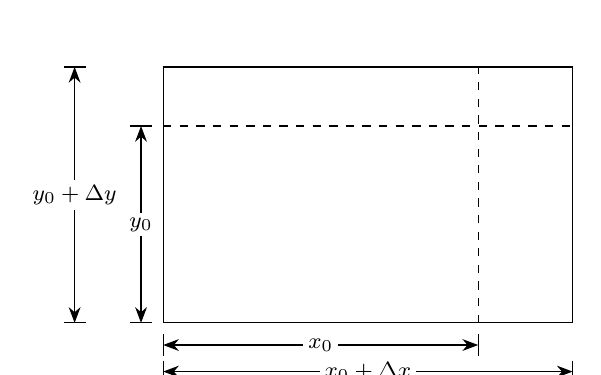
\begin{tikzpicture}[scale=1]
\def\w{4}
\def\h{2.5}
\def\s{1.3}

\coordinate (A) at (0,0);
\coordinate (B) at (\w,0);
\coordinate (C) at (\w,\h);
\coordinate (D) at (0,\h);
\coordinate (E) at ({\w*\s},0);
\coordinate (F) at ({\w*\s},\h);
\coordinate (G) at ({\w*\s},{\h*\s});
\coordinate (H) at (\w,{\h*\s});
\coordinate (K) at (0,{\h*\s});

% Location of points
% K    H   G
% D    C   F
% A    B   E

% The rectangle
\draw[-] (A) -| (G) -| cycle;
\draw[dashed] (B) -- (H);
\draw[dashed] (D) -- (F);

% Line labels, horizontal
\def\offy{-8pt}
\draw[<->] ([shift={(0pt,\offy)}]A)  
  -- node[fill=white,inner sep=1.8pt]{$x_0$} 
  ([shift={(0pt,\offy)}]B);
\draw[<->] ([shift={(0pt,{2.2*\offy})}]A)  
  -- node[fill=white,inner sep=1.8pt]{$x_0+\De x$} 
  ([shift={(0pt,{2.2*\offy})}]E);
\draw[-] ([shift={(0pt,{0.5*\offy})}]A) -- ([shift={(0pt,{1.5*\offy})}]A);
\draw[-] ([shift={(0pt,{0.5*\offy})}]B) -- ([shift={(0pt,{1.5*\offy})}]B);
\draw[-] ([shift={(0pt,{1.7*\offy})}]A) -- ([shift={(0pt,{2.7*\offy})}]A);
\draw[-] ([shift={(0pt,{1.7*\offy})}]E) -- ([shift={(0pt,{2.7*\offy})}]E);

% Line labels, vertical
\def\offx{-8pt}
\draw[<->] ([shift={(\offx, 0)}]A)  
  -- node[fill=white,inner sep=1.8pt]{$y_0$} 
  ([shift={(\offx,0)}]D);
\draw[<->] ([shift={({4*\offx}, 0)}]A)  
  -- node[fill=white,inner sep=1.8pt]{$y_0+\De y$} 
  ([shift={({4*\offx},0)}]K);

\draw[-] ([shift={({0.5*\offx},0pt)}]A) -- ([shift={({1.5*\offx},0pt)}]A);
\draw[-] ([shift={({0.5*\offx},0pt)}]D) -- ([shift={({1.5*\offx},0pt)}]D);
\draw[-] ([shift={({3.5*\offx},0pt)}]A) -- ([shift={({4.5*\offx},0pt)}]A);
\draw[-] ([shift={({3.5*\offx},0pt)}]K) -- ([shift={({4.5*\offx},0pt)}]K);
\end{tikzpicture}
\end{center}
\end{question}

\begin{solution}
The area function is $f(x,y) = xy$. The area of the new rectangle is
\[
f(x_0 + \De x, y_0 + \De y) =  x_0y_0 + y_0 \De x + x_0 \De y + \De x \De y\,,
\]
and thus the increase in the area is $y_0 \De x + x_0 \De + \De x \De y$. 

The linear approximation to $f$ at the point $(x_0, y_0)$ is
\[
\ell(x,y) = x_0 y_0 + y_0 (x - x_0) + x_0 (y-y_0)\,.
\]
Therefore the approximation of the area using the linear approximation is
\[
\ell(x_0+ \De x, y_0 + \De y) = x_0 y_0 + y_0 \De x + x_0 \De\,,
\]
and the approximation of the increase is $y_0 \De x + x_0 \De$.

\begin{center}
\begin{tabu} to \linewidth {X[1,c] X[1,c]}
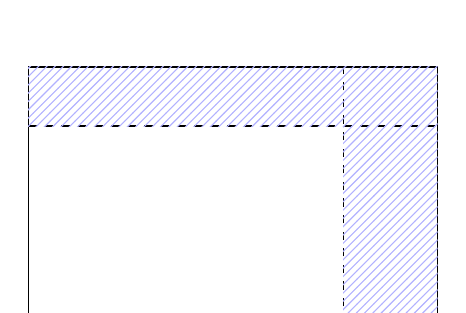
\begin{tikzpicture}[scale=1]
\def\w{4}
\def\h{2.5}
\def\s{1.3}

\coordinate (A) at (0,0);
\coordinate (B) at (\w,0);
\coordinate (C) at (\w,\h);
\coordinate (D) at (0,\h);
\coordinate (E) at ({\w*\s},0);
\coordinate (F) at ({\w*\s},\h);
\coordinate (G) at ({\w*\s},{\h*\s});
\coordinate (H) at (\w,{\h*\s});
\coordinate (K) at (0,{\h*\s});

% Location of points
% K    H   G
% D    C   F
% A    B   E

% The rectangle
\draw[-] (A) -| (G) -| cycle;
\draw[dashed] (B) -- (H);
\draw[dashed] (D) -- (F);
\fill[pattern color=blue!30, pattern=north east lines] (D) -| (H) -| cycle;
\fill[pattern color=blue!30, pattern=north east lines] (B) -| (F) -| cycle;
\fill[pattern color=blue!30, pattern=north east lines] (C) -| (G) -| cycle;
\end{tikzpicture} &
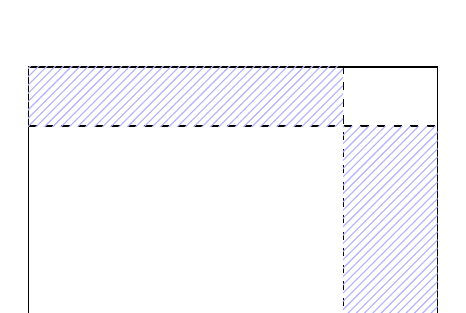
\begin{tikzpicture}[scale=1]
\def\w{4}
\def\h{2.5}
\def\s{1.3}

\coordinate (A) at (0,0);
\coordinate (B) at (\w,0);
\coordinate (C) at (\w,\h);
\coordinate (D) at (0,\h);
\coordinate (E) at ({\w*\s},0);
\coordinate (F) at ({\w*\s},\h);
\coordinate (G) at ({\w*\s},{\h*\s});
\coordinate (H) at (\w,{\h*\s});
\coordinate (K) at (0,{\h*\s});

% Location of points
% K    H   G
% D    C   F
% A    B   E

% The rectangle
\draw[-] (A) -| (G) -| cycle;
\draw[dashed] (B) -- (H);
\draw[dashed] (D) -- (F);
\fill[pattern color=blue!30, pattern=north east lines] (D) -| (H) -| cycle;
\fill[pattern color=blue!30, pattern=north east lines] (B) -| (F) -| cycle;
\end{tikzpicture} \\
Increase in area &
Increase in area using the linear approximation
\end{tabu}
\end{center}
\end{solution}

\begin{question}
The volume of a right circular cone of radius $r$ and height $h$ is given by $V=\frac 13 \pi r^2 h$. Suppose that the height decreases from $20\six{\cm}$ to $19.95\six{\cm}$ and the radius increases from $4\six{\cm}$ to $4.05\six{cm}$. Compare the change in volume of the cone with the estimate given by the linear approximation.
\end{question}

\begin{solution}
Write $V(r,h)$ for the volume of the cone to emphasize that it is a function of both radius $r$ and height $h$. The volume of the old cone is $V(20, 4) = 1675.52\six{cm^3}$ and the volume of the new cone is $V(19.95, 4.05) = 1687.99\six{cm^3}$. The change of volume is thus
\[
V(19.95, 4.05) - V(20,4) = 12.47\,.
\]
The partial derivatives of $V$ are
\begin{align*}
V_r(r,h) &= \frac 23 \pi r h &
V_h(r,h) &= \frac 13 \pi r^2\,,
\end{align*}
and $V_r(20,4) = 167.55$, $V_h(20,4) = 418.88$. The linear approximation of $V$ at $(20,4)$ is
\begin{align*}
\ell(r,h) &= V(20,4) + V_r(20,4)(r-20) + V_h(20,4)(h-4)\,.
\end{align*}
Therefore the approximate volume of the new cone is
\[
\ell(19.95, 4.05) = 1675.52 - 167.55 \cdot 0.05 + 418.88 \cdot 0.05 = 1688.09\,.
\]
The approximate change of volume is thus
\[
\ell(19.95, 4.05) - V(20,4) = 12.57\,.
\]
\end{solution}



%%% Local Variables:
%%% TeX-master: "problems"
%%% End:

\ifthenelse{\boolean{sectionnewpage}}{\newpage}{}
% Version: v1

\section{The Chain Rule}
\begin{question}
Suppose that a duck is swimming along a curve $x=3+2t$, $y=2-t^2$, while the water temperature is given by the formula $T = e^x(x + y)$. Find 
$\frac{dT}{dt}$ in two ways:
\begin{enumerate}
\item
by the chain rule and
\item
by expressing $T$ in terms of $t$ and differentiating.
\end{enumerate}
\end{question}

\begin{solution}
Note that we write $\frac{\p T}{\p x}$ and $\frac{\p T}{\p y}$, because $T(x,y)$ is a function of two variables. After subsituting $T(t)$ is a function of one variable and therefore we write $\frac{dT}{dt}$.
\begin{enumerate}
\item
By the chain rule the temperature of the duck is given by
\[
\frac{dT}{dt} = \frac{\p T}{\p x}\frac{dx}{dt} + \frac{\p T}{\p y} \frac{dy}{dt}\,.
\]
We have
\begin{align*}
\frac{\p T}{\p x} &= e^x(1 + x + y) &
\frac{\p T}{\p y} &= e^x\,,
\end{align*}
and after substitution
\begin{align*}
\frac{\p T}{\p x} 
&= e^{3+2t}\left(6 + 2t - t^2\right) &
\frac{\p T}{\p y} 
&= e^{3 + 2t}\,.
\end{align*}
The derivatives of $x(t)$ and $y(t)$ are
\begin{align*}
\frac{dx}{dt} &= 2 &
\frac{dy}{dt} &= -2t \,.
\end{align*}
Therefore
\begin{align*}
\frac{\p T}{\p x}\frac{dx}{dt} + \frac{\p T}{\p y} \frac{dy}{dt}
&= e^{3+2t}\left(12 + 2t - 2t^2\right)\,,
\end{align*}
by the chain rule.
\item
If we express $T$ as a function of $t$, we get
\[
T(t) = e^{3+2t}\left(5 + 2t - t^2\right)\,,
\]
and differentiating it leads to
\begin{align*}
\frac{dT}{dt} &= e^{3+2t} \left( 2 \left(5 + 2t - t^2\right) + 2 - 2t \right) \\
&= e^{3+2t} \left(12 + 2t - 2t^2 \right)\,.
\end{align*}
We see that both method lead to the same result.
\end{enumerate}
\end{solution}

\begin{question}
Suppose that a bird flies along a helical curve $x=2 \cos t$, $y = 2 \sin t$, $z=3t$. The bird suddenly encounters a weather front, so that the barometric pressure is varying rather wildly from point to point as $P(x,y,z) = \frac 3{10}\frac{x^2 z}{y} \,\textrm{atm}$.
\begin{enumerate}
\item
Use the chain rule to determine how the pressure is changing at $t = \frac \pi 4 \,\textrm{min}$.
\item
Using the linear approximation, determine the approximate pressure at $t=\frac \pi 4 + 0.01 \,\textrm{min}$.
\end{enumerate}
\end{question}

\begin{solution}
Note that we can ignore the physical units for most of the calculations, but we will use them to state the answer.
\begin{enumerate}
\item
The partial derivatives of $P(x,y,z)$ are
\begin{align*}
\frac{\p P}{\p x} &= \frac 35 \frac{xz}y &
\frac{\p P}{\p y} &= -\frac 3{10} \frac{x^2z}{y^2} &
\frac{\p P}{\p z} &= \frac 3{10} \frac{x^2}y\,,
\end{align*}
and the derivative of the bird's trajectory is
\begin{align*}
\frac{d x}{x t} &= -2 \sin t &
\frac{d y}{x t} &= 2 \cos t &
\frac{d z}{x t} &= 3 \,.
\end{align*}
The chain rule now gives
\begin{align*}
\frac{dP}{dt} &= \frac{9t}5 \frac {\cos t}{\sin t} \cdot (-2) \sin t
- \frac {9t}{10} \frac{\cos^2 t}{\sin^2 t} \cdot 2 \cos t
+ \frac 35 \frac{\cos^2t}{\sin t} \cdot 3 \\
&= -\frac{18t}5 \cos t - \frac{9t}{5} \frac{\cos^3 t}{\sin^2 t}
+ \frac 95 \frac{\cos^2t}{\sin t}\,.
\end{align*}
Evaluated at $t=\frac \pi 4$ we obtain
\[
\frac{dP}{dt}\left(\frac \pi 4\right) = -\frac{9\sqrt{2}}{10}\left(-\frac{3\pi}{4} + 1\right)
\approx - 1.726\ldots\,.
\]
Therefore at $\frac \pi 4 \,\textrm{min}$ the barometric pressure changes at a rate of $-1.726 \,\frac{\textrm{atm}}{\textrm{min}}$.

\item
First we evaluate
\[
P(\left(\frac \pi 4 \right) = \frac{9\pi\sqrt 2}{40} \approx 0.9996\ldots
\]
The linear approximation tells us that
\begin{align*}
P\left( \frac \pi 4 + 0.01 \right) &\approx P\left(\frac \pi 4 \right) 
+ \frac{dP}{dt}\left(\frac \pi 4 \right) \cdot 0.01 \\
&\approx 0.9996 - 1.726 \cdot 0.01 \approx 0.9823\,.
\end{align*}
\end{enumerate}
The problem is stated in physical units, so it is natural to enquire, whether the numbers make sense. At $t=\frac \pi 4 \,\textrm{min}$ the barometric pressure is $0.9996 \,\textrm{atm}$, which is average sea-level pressure. How much does pressure change over time? The highest recorded barometric presssure is about $1.08 \,\textrm{atm}$ and the lowest pressures occur during typhoons and are about $0.86 \,\textrm{atm}$. Hence a rate of change of $-1.726 \,\frac{\textrm{atm}}{\textrm{min}}$ would indicate an extremely rapid decrease.
\end{solution}

\begin{question}
Use the chain rule to determine an expression for the indicated derivative.
\begin{enumerate}
\item
Let $z=\sqrt{x^2+y^2}+2xy^2$, where $x$ and $y$ are functions of $u$. Find an expression for $\frac{dz}{du}$.
\item
Let $u =\sin\left(a + \ln b\right)$, where $a$ and $b$ are functions of $t$. Find an expression for $\frac{du}{dt}$.
\end{enumerate}
\end{question}

\begin{solution}
\begin{enumerate}
\item
The chain rule states that
\[
\frac{dz}{du} = \frac{\p z}{\p x}\frac{dx}{du}
+ \frac{\p z}{\p y}\frac{dy}{du}\,.
\]
The partial derivatives of $z=z(x,y)$ are
\begin{align*}
\frac{\p z}{\p x} &=
\frac{x}{\sqrt{x^2+y^2}} + 2y^2 &
\frac{\p z}{\p y} &=
\frac{y}{\sqrt{x^2+y^2}} + 4xy\,.
\end{align*}
Hence
\[
\frac{dz}{du} = \frac{1}{\sqrt{x^2+y^2}}
\left( x \frac{dx}{du} + y \frac{dy}{du} \right)
+ 2y^2 \frac{dx}{du} + 4xy \frac{dy}{du}\,.
\]
\item
The chain rule states that
\[
\frac{du}{dt} = \frac{\p u}{\p a}\frac{da}{dt}
+ \frac{\p u}{\p b}\frac{db}{dt}\,.
\]
The partial derivatives of $u=u(a,b)$ are
\begin{align*}
\frac{\p u}{\p a} &=
\cos(a + \ln b) &
\frac{\p u}{\p b} &=
\frac 1b \cos(a + \ln b) \,.
\end{align*}
Hence
\[
\frac{du}{dt} = \cos(a + \ln b) 
\left( \frac{da}{dt} + \frac 1b \frac{db}{dt} \right)\,.
\]
\end{enumerate}
\end{solution}

\begin{question}
For the following functions, calculate the derivative $\frac{d}{dt}\left(f \circ \bm{\si} \right)$ using the chain rule.
\begin{enumerate}
\item
$f(x,y) = (x^2+y^2)\ln\left(\sqrt{x^2+y^2}\right)$;
$\bm\si(t) = (e^t, e^{-t})$.
\item
$f(x,y) = xe^{x^2+y^2}$;
$\bm\si(t) = (t,-t)$.
\item
$f(x,y,z) = x+y^2+z^3$;
$\bm\si(t) = (\cos t, \sin t, t)$.
\item
$f(x,y,z) = e^{x-z}(y^2-x^2)$;
$\bm\si(t) = (t, e^t, t^2)$.
\end{enumerate}
\end{question}

\begin{solution}
We will write $\bm \si = (\si_1, \si_2)$ for the components of the curve $\bm \si$. Thus if $\bm \si(t) = (e^t, e^{-t})$, then $\si_1(t) = e^t$ and $\si_2(t) = e^{-t}$.
\begin{enumerate}
\item
The partial derivatives of $f$ are
\begin{align*}
f_x &= x \left( 2 \ln \sqrt{x^2+y^2} +\sqrt{x^2+y^2} \right) &
f_y &= y \left( 2 \ln \sqrt{x^2+y^2} +\sqrt{x^2+y^2} \right)\,,
\end{align*}
and
\[
\bm \si'(t) = \left(e^t, -e^{-t}\right)\,.
\]
Thus
\begin{align*}
\frac{d}{dt}\left(f \circ \bm \si\right) &=
e^t \left( 2 \ln \sqrt{ e^{2t} + e^{-2t}} + \sqrt{ e^{2t} + e^{-2t}} \right) \cdot e^t \\
&\qquad{} +
e^{-t} \left( 2 \ln \sqrt{ e^{2t} + e^{-2t}} + \sqrt{ e^{2t} + e^{-2t}} \right) \cdot \left(-e^{-t}\right) \\
&= \left(e^{2t}-e^{-2t}\right) \left(2\ln \sqrt{e^{2t}+e^{-2t}} + \sqrt{e^{2t}+e^{-2t}} \right)\,.
\end{align*}

\item
The partial derivatives of $f$ are
\begin{align*}
f_x &= (1 + 2x^2)e^{x^2+y^2} &
f_y &= 2xy e^{x^2+y^2}\,,
\end{align*}
and
\[
\bm \si'(t) = (1,-2)\,.
\]
Thus
\begin{align*}
\frac{d}{dt}\left(f \circ \bm \si\right) &=
 (1 + 2t^2)e^{2t^2} \cdot 1 - 2t^2 e^{2t^2} \cdot (-1) = \left( 1 + 4t^2 \right) e^{2t^2} \,.
\end{align*}

\item
The partial derivatives of $f$ are
\begin{align*}
f_x &= 1 &
f_y &= 2y &
f_z &= 3z^2\,,
\end{align*}
and
\[
\bm \si'(t) = (-\sin t, \cos t, 1)\,.
\]
Thus
\begin{align*}
\frac{d}{dt}\left(f \circ \bm \si\right) &=
 1 \cdot \left( - \sin t\right) + 2\sin t \cdot \cos t + 3t^2 \cdot 1
= -\sin t + 2 \sin t \cos t + 3t^2\,.
\end{align*}

\item
The partial derivatives of $f$ are
\begin{align*}
f_x &= e^{x-z}(y^2-2x-x^2) &
f_y &= 2ye^{x-z} &
f_z &= -e^{x-z}(y^2-x^2)\,.
\end{align*}
and
\[
\bm\si'(t) = (1, e^t, 2t)\,.
\]
Thus
\begin{align*}
\frac{d}{dt}\left(f \circ \bm \si\right) &=
 e^{t-t^2}\left(e^{2t}-2t-t^2\right) \cdot 1 + 2e^{t} e^{t-t^2} \cdot e^t
- e^{t-t^2} \left(e^{2t}-t^2\right) \cdot 2t \\
&= (3-2t)e^{3t-t^2} - (2t+t^2-2t^3)e^{t-t^2}\,.
\end{align*}
\end{enumerate}
\end{solution}

\begin{question}
In this problem we will use the chain rule to rederive results from single-variable calculus.
\begin{enumerate}
\item
Apply the chain rule to the function $u=xyz$, where $x=x(t)$, $y=y(t)$ and $z=z(t)$ are functions of $t$ to get a rule for differentiating a product of three functions of one variable.
\item
Use the chain rule and the function $f(y,z) = y^z$ to find $\displaystyle\frac{d}{dx}\left( x^x \right)$.
\end{enumerate}
\end{question}

\begin{solution}
\begin{enumerate}
\item
The chain rule gives
\[
\frac{du}{dt} = \frac{\p u}{\p x}\frac{dx}{dt}
+ \frac{\p u}{\p y}\frac{dy}{dt}
+ \frac{\p u}{\p z}\frac{dz}{dt} \,.
\]
The partial derivatives are
\begin{align*}
\frac{\p u}{\p x} &= yz &
\frac{\p u}{\p y} &= xz &
\frac{\p u}{\p z} &= xy\,,
\end{align*}
and hence
\[
\frac{du}{dt} = \frac{dx}{dt} yz
+ x \frac{dy}{dt} z
+ xy\frac{dz}{dt} \,,
\]
which is the product rule for a product of three factors. A more common form would be
\[
(fgh)' = f' gh + fg'h + fgh'\,.
\]
\item
If we consider $y(x)=x$ and $z(x)=x$ as functions of $x$, then
\[
x^x = f(x,x)\,,
\]
where $f(y,z) = y^z$. Using the chain rule we have
\[
\frac{d}{dx}\left( x^x \right) =
\frac{\p f}{\p y}\frac{dy}{dx} + 
\frac{\p f}{\p z}\frac{dz}{dx}\,.
\]
To compute the partial derivatives of $f$ we make the following observation: keeping $z$ fixed we can differentiate $y^z$ like a polynomial; keeping $y$ fixed we can write $y = e^{\ln y}$ and thus $y^z = e^{z \ln y}$. Therefore the partial derivatives of $f(y,z)$ are
\begin{align*}
\frac{\p f}{\p y} &= zy^{z-1} &
\frac{\p f}{\p z} &= y^z \ln y\,,
\end{align*}
and both $\frac{dy}{dx} = 1$ and $\frac{dz}{dx} = 1$. Thus
\[
\frac{d}{dx}\left( x^x \right) = x x^{x-1} + x^x \ln x = x^{x} \left( 1 + \ln x\right)\,.
\]
\end{enumerate}
\end{solution}

\begin{question}
Let $F(u,v)$ be a function of two variables. Suppose that $u = x+y$ and $v=xy$. Express $\frac{\p^2 F}{\p x \p y}$ in terms of $u$- and $v$-derivatives of $F$.
\end{question}

\begin{solution}
We first compute $\frac{\p F}{\p x}$ and $\frac{\p F}{\p y}$,
\begin{align*}
\frac{\p F}{\p x} &= \frac{\p F}{\p u} + y\frac{\p F}{\p v} &
\frac{\p F}{\p x} &= \frac{\p F}{\p u} + x\frac{\p F}{\p v}\,.
\end{align*}
Note that these formulas are valid for all functions $F(u,v)$. In particular we can replace $F$ by $\frac{\p F}{\p y}$,
\begin{align*}
\frac{\p}{\p x}\frac{\p F}{\p y} &=
\frac{\p}{\p x}\left(\frac{\p F}{\p u} + x\frac{\p F}{\p v}\right) \\
&= \frac{\p^2 F}{\p u^2} + y\frac{\p^2 F}{\p v \p u}
+ \frac{\p F}{\p v}
+ x \left( \frac{\p^2 F}{\p u \p v} + y\frac{\p^2 F}{\p v^2} \right) \\
&= \frac{\p F}{\p v} + \frac{\p^2 F}{\p u^2} 
+ (x + y) \frac{\p^2 F}{\p u \p v} + x y\frac{\p^2 F}{\p v^2}\,.
\end{align*}
When calculating $\frac{\p}{\p x} \left( x \frac{\p F}{\p v} \right)$ we had to apply the product rule. Differentiating the first factor gives $\frac{\p}{\p x}(x) = 1$ and for the second factor we use the result from above, which was obtained using the chain rule.
\end{solution}

\begin{question}
Let $u(x, y, z)$ be a function of three variables. Suppose that $x = pq^2 r$, $y = pq^3$ and $z = p^3$. Express $\frac{\p^2 u}{\p p \p r}$ in terms of $x$-, $y$- and $z$-derivatives of $u$.
\end{question}

\begin{solution}
We start with the first derivatives
\begin{align*}
\frac{\p u}{\p p} &= q^2 r \frac{\p u}{\p x} + q^3 \frac{\p u}{\p y}
+ 3p^2 \frac{\p u}{\p z} &
\frac{\p u}{\p r} &= pq^2 \frac{\p u}{\p x}\,.
\end{align*}
We do not need the $q$-derivative in this problem. Then
\begin{align*}
\frac{\p^2 u}{\p p \p r} &= \frac{\p}{\p p} \left(pq^2\right) \frac{\p u}{\p x} 
+ pq^2\left( q^2 r \frac{\p^2 u}{\p x^2} + q^3 \frac{\p^2 u}{\p y \p x}
+ 3p^2 \frac{\p^2 u}{\p z \p x} \right) \\
&= q^2 \frac{\p u}{\p x} 
+ pq^4 r \frac{\p^2 u}{\p x^2} + pq^5 \frac{\p^2 u}{\p x \p y}
+ 3p^3q^2 \frac{\p^2 u}{\p x \p z}\,.
\end{align*}
\end{solution}

\begin{question}
Cartesian (rectangular) coordinates $(x,y)$ of a point can be expressed in terms of polar coordinates $(r,\th)$ using the expressions
\begin{align*}
x &= r \cos \th &
y &= r \sin \th\,.
\end{align*}
Suppose that a function is given in terms of cartesian coordinates by $u=f(x,y)$. 
\begin{enumerate}
\item
Express $\frac{\p u}{\p r}$ and $\frac{\p u}{\p \th}$ in terms of
$\frac{\p u}{\p x}$ and $\frac{\p u}{\p y}$.
\item
Show that
\[
u_x^2 + u_y^2 = u_r^2 + \frac 1{r^2} u_\th^2\,.
\]
\item
Express
\[
u_{rr} + \frac 1r u_r + \frac 1{r^2} u_{\th\th}
\]
in cartesian coordinates.
\end{enumerate}
\end{question}

\begin{solution}
The derivative of $(x,y)$ with respect to $(r,\th)$ is
\begin{align*}
\frac{\p x}{\p r} &= \cos \th & \frac{\p x}{\p \th} &= -r \sin \th \\
\frac{\p y}{\p r} &= \sin \th & \frac{\p y}{\p \th} &= r \cos \th\,.
\end{align*}
\begin{enumerate}
\item
We can do this by simply applying the chain rule
\begin{align*}
\frac{\p u}{\p r} &= \cos \th \frac{\p u}{\p x} + \sin \th \frac{\p u}{\p y} \\
\frac{\p u}{\p \th} &= -r \sin\th \frac{\p u}{\p x} + r\cos \th \frac{\p u}{\p y}\,.
\end{align*}

\item
We start with the right hand side of the sought after identity,
\begin{align*}
u_r^2 + \frac 1{r^2} u_\th^2
&= \left(\cos \th\,u_x + \sin\th \, u_y\right)^2
+ \frac{1}{r^2} \left( -r\sin \th\, u_x + r \cos \th \,u_y\right)^2 \\
&= \left(\cos^2 \th + \sin^2 \th\right) u_x^2 + 
\left(\cos^2 \th + \sin^2 \th\right) u_y^2
= u_x^2 + u_y^2\,.
\end{align*}

Please note the difference between $u_x^2$ and $(u^2)_x$ and $u_{xx}$. By $u_x^2$ we mean the square of the function $u_x$, in other words $u_x^2 = (u_x)^2$. On the other hand $(u^2)_x$ is the $x$-derivative of the square $u^2$ and one has $(u^2)_x = 2uu_x$. Finally $u_{xx}$ is the second partial derivative. These are in general different functions.

\item
In order to express $u_{rr} + \frac 1r u_r + \frac{1}{r^2}u_{\th\th}$ in cartesian coordinates we need expressions for the second derivatives. First we have
\begin{align*} 
\frac{\p^2 u}{\p r^2}
&= \frac{\p}{\p r} \left( \cos \th\right) \frac{\p u}{\p x}
+ \cos \th \left( \cos \th \frac{\p^2 u}{\p x^2} + 
\sin \th \frac{\p^2 u}{\p y \p x} \right) \\
&\qquad + \frac{\p}{\p r} \left( \sin \th\right) \frac{\p u}{\p y}
+ \sin \th \left( \cos \th \frac{\p^2 u}{\p x \p y} + 
\sin \th \frac{\p^2 u}{\p y^2} \right) \\
&= \cos^2 \th \frac{\p^2 u}{\p x^2} + 2\sin \th \cos \th \frac{\p^2 u}{\p x \p y}
+ \sin^2 \th \frac{\p^2 u}{\p y^2}\,.
\end{align*}
Next is the second $\th$-derivative,
\begin{align*}
\frac{\p^2 u}{\p \th^2}
&= \frac{\p}{\p \th} \left( -r \sin \th\right) \frac{\p u}{\p x}
-r\sin \th \left(-r \sin \th \frac{\p^2 u}{\p x^2} + 
r \cos \th \frac{\p^2 u}{\p y \p x} \right) \\
&\qquad{} + \frac{\p}{\p \th} \left( r \cos \th\right) \frac{\p u}{\p y}
+ r \cos \th \left( -r\sin \th \frac{\p^2 u}{\p x \p y} + 
r \cos \th \frac{\p^2 u}{\p y^2} \right) \\
&= -r\cos \th \frac{\p u}{\p x} - r \sin \th \frac{\p u}{\p y}
+ r^2 \sin^2 \th \frac{\p^2 u}{\p x^2} - 2r^2 \sin \th \cos \th \frac{\p^2 u}{\p x \p y}
+ r^2 \cos^2 \th \frac{\p^2 u}{\p y^2}\,.
\end{align*}
The required sum is
\begin{align*}
u_{rr} + &\frac{1}{r} u_r + \frac{1}{r^2} u_{\th\th} = \\
&= \left( \cos^2 \th \, u_{xx} + 2 \sin \th \cos \th \, u_{xy}
+ \sin^2 \th \, u_{yy} \right)
+ \frac{1}{r} \left( \cos \th \, u_x + \sin \th \, u_y \right) \\
&\qquad{} + \frac{1}{r^2} \left( -r\cos \th \, u_x - r \sin \th \, u_y 
+ r^2 \cos^2 \th \, u_{xx} - 2r^2 \sin \th \cos \th \, u_{xy} 
+ r^2 \cos^2 \th \, u_{yy} \right) \\
&= \left( \cos^2 \th + \sin^2 \th \right) u_{xx} + 
\left( \cos^2 \th + \sin^2 \th \right) u_{yy}
= u_{xx} + u_{yy}\,.
\end{align*}
Therefore $u_{rr} + \frac 1r u_r + \frac{1}{r^2}u_{\th\th}$ becomes $u_{xx} + u_{yy}$ in cartesian coordinates.
\end{enumerate}
\end{solution}

\begin{question}
Compute the following derivative matrices and evaluate them at the given points.
\begin{enumerate}
\item
$\frac{\p(x,y)}{\p(u,v)}$, where
$x = u \sin v$, $y = e^{uv}$; evaluate at $(0,1)$.
\item
$\frac{\p(x,y,z)}{\p(r,\th,\ph)}$, where
$x = r\sin \ph \cos \th$, $y = r \sin \ph \sin \th$, $z = r \cos \ph$; evaluate at 
$\left(4, \frac\pi 4, \frac \pi 4\right)$.
\item
$\frac{\p(u,v)}{\p(x,y,z)}$, where
$u = xyz$, $v = x+y+z$; evaluate at $(1, 2, 3)$.
\end{enumerate}
\end{question}

\begin{solution} It is important to remember the order of partial derivatives in the derivative matrix.
\begin{enumerate}
\item
We have
\begin{align*}
\frac{\p(x,y)}{\p(u,v)} &=
\begin{pmatrix}
\sin v & u \cos v \\
v e^u & u e^v
\end{pmatrix} &
\frac{\p(x,y)}{\p(u,v)}(0,1) &=
\begin{pmatrix}
\sin 1 & 0 \\
1 & 0
\end{pmatrix}\,.
\end{align*}
\item
We have
\begin{align*}
\frac{\p(x,y,z)}{\p(r,\th,\ph)} &=
\begin{pmatrix}
\sin \ph \cos \th & -r \sin \ph \sin \th & r \cos \ph \cos \th \\
\sin \ph \sin \th & r \sin \ph \cos \th & r \cos \ph \sin \th \\
\cos \ph & 0 & -r \sin \ph
\end{pmatrix}\,.
\end{align*}
To evaluate at $\left(4, \frac \pi4, \frac \pi4\right)$ we use that $\sin \frac \pi4 = \frac{\sqrt 2}2$ and $\cos \frac \pi 4 = \frac{\sqrt 2}{2}$ and hence
\[
\frac{\p(x,y,z)}{\p(r,\th,\ph)}\left(4, \frac \pi 4, \frac \pi 4\right) =
\begin{pmatrix}
\tfrac 12 & -1 & 1 \\
\tfrac 12 & 1 & 1 \\
\tfrac{\sqrt 2}2 & 0 & -2
\end{pmatrix} \,.
\]

\item
We have
\begin{align*}
\frac{\p(u,v)}{\p(x,y,z)} &=
\begin{pmatrix}
yz & xz & xy \\
1 & 1 & 1
\end{pmatrix} &
\frac{\p(u,v)}{\p(x,y,z)}(1, 2, 3) &=
\begin{pmatrix}
6 & 3 & 2 \\
1 & 1 & 1
\end{pmatrix}\,.
\end{align*}
\end{enumerate}
\end{solution}

% \begin{question}
% Verify the general chain rule for each of the functions by following these steps:
% \begin{enumerate}[(i)]
% \item
% Compute the derivative matrices
% $\displaystyle\frac{\p(x,y)}{\p(t,s)}$ and
% $\displaystyle\frac{\p(u,v)}{\p(x,y)}$;
% \item
% Express $(u,v)$ in terms of $(t,s)$ and calculate
% $\displaystyle\frac{\p(u,v)}{\p(t,s)}$;
% \item
% Verify that the chain rule holds.
% \end{enumerate}
% Do this for the following functions:
% \begin{enumerate}
% \item
% $
% \begin{aligned}
% x &= t+s \\
% y &= t-s
% \end{aligned}
% \quad\text{ and }\quad
% \begin{aligned}
% u &= x^2 + y^2 \\
% v &= x^2 - y^2
% \end{aligned}
% \,.$

% \item
% $
% \begin{aligned}
% x &= t^2-s^2 \\
% y &= ts
% \end{aligned}
% \quad\text{ and }\quad
% \begin{aligned}
% u &= \sin(x+y) \\
% v &= \cos(x-y)
% \end{aligned}
% \,.$

% \item
% $
% \begin{aligned}
% x &= t^2+s^2 \\
% y &= t^2-s^2 \\
% z &= 2ts
% \end{aligned}
% \quad\text{ and }\quad
% \begin{aligned}
% u &= xy \\
% v &= yz \\
% w &= xz
% \end{aligned}
% $
% \end{enumerate}
% \end{question}

% \begin{solution}
% The chain rule states that
% \[
% \frac{\p(u,v)}{\p(t,s)} = \frac{\p(u,v)}{\p(x,y)}(t,s) \cdot \frac{\p(x,y)}{\p(t,s)}\,,
% \]
% where $\frac{\p(u,v)}{\p(x,y)}(t,s)$ denotes the Jacobi matrix of the functions $(u,v)$ with respect to $(x,y)$, but evaluated in the $(t,s)$ variables.

% \begin{enumerate}[(a)]
% \item
% Following the steps we have
% \begin{enumerate}[(i)]
% \item
% \begin{align*}
% \frac{\p (u,v)}{\p (x,y)} &=
% \begin{pmatrix}
% 2x & 2y \\
% 2x & -2y
% \end{pmatrix} &
% \frac{\p (u,v)}{\p (x,y)}(t,s) &=
% \begin{pmatrix}
% 2(t+s) & 2(t-s) \\
% 2(t+s) & -2(t-s)
% \end{pmatrix} &
% \frac{\p (x,y)}{\p (t,s)} &=
% \begin{pmatrix}
% 1 & 1 \\
% 1 & -1
% \end{pmatrix}
% \end{align*}
% \item
% We have
% \begin{align*}
% u &= (t+s)^2 + (t-s)^2 = 2t^2 + 2s^2\\
% v &= (t+s)^2 - (t-s)^2 = 4ts
% \end{align*}
% and the Jacobi matrix is
% \[
% \frac{\p (u,v)}{\p (t,s)} =
% \begin{pmatrix}
% 4t & 4s \\
% 4s & 4t
% \end{pmatrix}
% \]
% \item
% To verify the chain rule we need to compute the matrix product
% \[
% \frac{\p(u,v)}{\p(x,y)}(t,s) \cdot \frac{\p(x,y)}{\p(t,s)} = 
% \begin{pmatrix}
% 2(t+s) & 2(t-s) \\
% 2(t+s) & -2(t-s)
% \end{pmatrix} \cdot
% \begin{pmatrix}
% 1 & 1 \\
% 1 & -1
% \end{pmatrix}
% = \begin{pmatrix}
% 4t & 4s \\
% 4s & 4t
% \end{pmatrix}\,.
% \]
% \end{enumerate}

% \item
% Following the steps we have
% \begin{enumerate}[(i)]
% \item
% \begin{align*}
% \frac{\p (u,v)}{\p (x,y)} &\!=\!
% \begin{pmatrix}
% \cos(x+y) & \!\!\!\cos(x+y) \\
% -\sin(x-y) & \!\!\! \sin(x-y)
% \end{pmatrix} &\!\!\!\!
% \frac{\p (u,v)}{\p (x,y)}(t,s) &\!=\!
% \begin{pmatrix}
% \cos(t^2-s^2+ts) & \!\!\!\cos(t^2-s^2+ts) \\
% -\sin(t^2-s^2-ts) & \!\!\! \sin(t^2-s^2-ts)
% \end{pmatrix} &\!\!\!\!
% \frac{\p (x,y)}{\p (t,s)} &\!=\!
% \begin{pmatrix}
% 2t & -2s \\
% s & t
% \end{pmatrix}
% \end{align*}
% \item
% We have
% \begin{align*}
% u &= \sin(t^2-s^2+ts)\\
% v &= \cos(t^2-s^2-ts)
% \end{align*}
% and the Jacobi matrix is
% \[
% \frac{\p (u,v)}{\p (t,s)} =
% \begin{pmatrix}
% (2t+s) \cos(t^2-s^2+ts) & (-2s+t) \cos(t^2-s^2+ts) \\
% -(2t-s)\sin(t^2-s^2-ts) & -(-2s-t)\sin(t^2-s^2-ts)
% \end{pmatrix}
% \]
% \item
% To verify the chain rule we need to compute the matrix product
% \begin{align*}
% \frac{\p(u,v)}{\p(x,y)}(t,s) \cdot \frac{\p(x,y)}{\p(t,s)} &= 
% \begin{pmatrix}
% \cos(t^2-s^2+ts) & \cos(t^2-s^2+ts) \\
% -\sin(t^2-s^2-ts) & \sin(t^2-s^2-ts)
% \end{pmatrix} \cdot
% \begin{pmatrix}
% 2t & -2s \\
% s & t
% \end{pmatrix} \\ &=
% \begin{pmatrix}
% (2t+s) \cos(t^2-s^2+ts) & (-2s+t) \cos(t^2-s^2+ts) \\
% (-2t+s)\sin(t^2-s^2-ts) & (2s+t)\sin(t^2-s^2-ts)
% \end{pmatrix}\,.
% \end{align*}
% \end{enumerate}

% \item
% Following the steps we have
% \begin{enumerate}[(i)]
% \item
% \begin{align*}
% \frac{\p (u,v,w)}{\p (x,y, z)} &=
% \begin{pmatrix}
% y & x & 0 \\
% 0 & z & y \\
% z & 0 & x
% \end{pmatrix} &
% \frac{\p (u,v,w)}{\p (x,y,z)}(t,s) &=
% \begin{pmatrix}
% t^2-s^2 & t^2+s^2 & 0 \\
% 0 & 2ts & t^2-s^2 \\
% 2ts & 0 & t^2+s^2
% \end{pmatrix} &
% \frac{\p (x,y,z)}{\p (t,s)} &=
% \begin{pmatrix}
% 2t & 2s \\
% 2t & -2s \\
% 2s & 2t
% \end{pmatrix}
% \end{align*}
% \item
% We have
% \begin{align*}
% u &= (t^2+s^2)(t^2-s^2) = t^4 - s^4\\
% v &= 2t^3 s - 2ts^3 \\
% z &= 2t^3 s + 2ts^3
% \end{align*}
% and the Jacobi matrix is
% \[
% \frac{\p (u,v,w)}{\p (t,s)} =
% \begin{pmatrix}
% 4t^3 & -4s^3 \\
% 6t^2s - 2s^3 & 2t^3 - 6ts^2 \\
% 6t^2s + 2s^3 & 2t^3 + 6ts^2
% \end{pmatrix}
% \]
% \item
% To verify the chain rule we need to compute the matrix product
% \begin{align*}
% \frac{\p(u,v,w)}{\p(x,y,z)}(t,s) \cdot \frac{\p(x,y,z)}{\p(t,s)} &= 
% \begin{pmatrix}
% t^2-s^2 & t^2+s^2 & 0 \\
% 0 & 2ts & t^2-s^2 \\
% 2ts & 0 & t^2+s^2
% \end{pmatrix} \cdot
% \begin{pmatrix}
% 2t & 2s \\
% 2t & -2s \\
% 2s & 2t
% \end{pmatrix} \\&=
% \begin{pmatrix}
% 4t^3 & -4s^3 \\
% 6t^2s - 2s^3 & 2t^3 - 6ts^2 \\
% 6t^2s + 2s^3 & 2t^3 + 6ts^2
% \end{pmatrix} \,.
% \end{align*}
% \end{enumerate}
% \end{enumerate}
% \end{solution}

% \begin{question}
% Cartesian (rectangular) coordinates $(x,y)$ of a point can be expressed in terms of polar coordinates $(r,\th)$ using the expressions
% \begin{align*}
% x &= r \cos \th &
% y &= r \sin \th\,.
% \end{align*}
% Suppose that a function is given in terms of cartesian coordinates by $u=f(x,y)$. 
% \begin{enumerate}[(a)]
% \item
% Calculate the derivative matrix $\displaystyle\frac{\p(x,y)}{\p (r,\th)}$.
% \item
% Suppose that a function is given in terms of cartesian coordinates by $u=f(x,y)$. Express
% $\displaystyle\frac{\p u}{\p r}$ and $\displaystyle\frac{\p u}{\p \th}$ in terms of
% $\displaystyle\frac{\p u}{\p x}$ and $\displaystyle\frac{\p u}{\p y}$.
% \item
% Let $u=x^2+y^2$. Find $\displaystyle\frac{\p u}{\p r}$ and 
% $\displaystyle\frac{\p u}{\p \th}$.
% \item
% Express the polar coordinates $r$, $\th$ in terms of the cartesian coordinates $x$, $y$ and find the derivative matrix $\displaystyle\frac{\p(r,\th)}{\p (x,y)}$
% \end{enumerate}
% \end{question}

% \begin{solution}
% \begin{enumerate}[(a)]
% \item
% The derivative matrix is given by
% \[
% \frac{\p(x,y)}{\p (r,\th)} = 
% \begin{pmatrix}
% \cos \th & -r\sin \th \\
% \sin \th & r \cos \th
% \end{pmatrix}\,.
% \]
% \item
% We have
% \begin{align*}
% \frac{\p u}{\p r} &=
% \frac{\p u}{\p x} \frac{\p x}{\p r} + \frac{\p u}{\p y} \frac{\p y}{\p r}
% = \frac{\p u}{\p x} \cos \th + \frac{\p u}{\p y} \sin \th \\
% \frac{\p u}{\p \th} &=
% \frac{\p u}{\p x} \frac{\p x}{\p \th} + \frac{\p u}{\p y} \frac{\p y}{\p \th}
% = - r \frac{\p u}{\p x} \sin \th + r \frac{\p u}{\p y} \cos \th \,.
% \end{align*}
% \item
% We have
% \begin{align*}
% r &= \sqrt{x^2 + y^2} \\
% \th &= \arctan \frac y x\,,
% \end{align*}
% and so
% \[
% \frac{\p(x,y)}{\p (r,\th)} = 
% \begin{pmatrix}
% \displaystyle\frac{x}{\sqrt{x^2+y^2}} & \displaystyle\frac{y}{\sqrt{x^2+y^2}} \\
% \displaystyle\frac{-y}{x^2+y^2} & \displaystyle\frac{x}{x^2+y^2} 
% \end{pmatrix}\,.
% \]
% \end{enumerate}
% \end{solution}


\begin{question}
{\bfseries Differentiating under the integral.}
Under mild continuity restrictions, it is true that if
\[
F(x) = \int_a^b g(t,x) \ud t\,,
\]
then
$\displaystyle F'(x) = \int_a^b g_x(t,x) \ud t$.
Using this fact and the chain rule we can find the derivative of
\[
F(x) = \int_a^{f(x)} g(t,x) \ud t
\]
by letting
\[
G(u,x) = \int_a^u g(t,x) \ud t\,,
\]
where $u = f(x)$. Find the derivatives of the following functions:
\begin{enumerate}
\item
$\displaystyle
F(x) = \int_0^{x^2} \sqrt{t^4 + x^3} \ud t\,.
$
\item
$\displaystyle
F(x) = \int_{x}^{1} x \ln(t^2+x^2) \ud t\,.
$
\end{enumerate}
\end{question}

\begin{solution}
With $G(u,x)$ defined as above we have
\[
F(x) = G(f(x), x)
\]
and we can find the derivative of $F$ using the chain rule,
\[
F'(x) = G_u(f(x),x) f'(x) + G_x(f(x),x)\,.
\]
We know from the problem statement, that
\[
G_x(u,x) = \int_a^u g_x(t,x) \ud t\,,
\]
and what we need know is the derivative $G_u(u,x)$. But this we obtain from the fundamental theorem of calculus, which states that
\[
\frac{d}{du} \int_a^u g(t,x) \ud t = g(u,x)\,,
\]
or in our notation, $G_u(u,x) = g(u,x)$. It means that differentiating an integral with respect to the upper limit results in the function we are integrating. Putting it all together we obtain
\begin{align*}
F'(x) &= G_u(f(x),x) f'(x) + G_x(f(x),x) \\
&= g(f(x), x) f'(x) + \int_a^{f(x)} g_x(t,x) \ud t\,.
\end{align*}

Now we are ready to attempt the problems.
\begin{enumerate}
\item
$F(x) = \int_0^{x^2} \sqrt{t^4 + x^3} \ud t$. Then
\[
F'(x) = \sqrt{x^8 + x^3} \cdot 2x + \frac 32 \int_0^{x^2} \frac{x^2}{\sqrt{t^4+x^3}} \ud t\,.
\]
\item
We rewrite $F(x)$ as 
$F(x) = \int_{x}^{1} x \ln\left(t^2 + x^2\right) \ud t = -\int_1^{x} x \ln\left(t^2 + x^2\right) \ud t$. Then
\begin{align*}
F'(x) &= -x \ln \left(x^2 + x^2\right) - \int_1^x \frac{2x^2}{t^2 + x^2} \ud t \\
&= -x \ln \left(2x^2 \right) + \int_x^1 \frac{2x}{t^2 + x^2} \ud t\,.
\end{align*}
\end{enumerate}
\end{solution}

%%% Local Variables:
%%% TeX-master: "problems"
%%% End:

\ifthenelse{\boolean{sectionnewpage}}{\newpage}{}
% Version: v1

\section{Gradients and Directional Derivatives}
\begin{question}
True or false: a partial derivative is a specific example of a directional derivative.
\end{question}

\begin{solution}
True.

For example, the partial derivative $f_x(a,b)$ at a point $(a,b)$ equals the directional derivative in the direction $\vec i$, since $f_x(a,b) = \nabla f(a,b) \cdot \vec i$.
\end{solution}

\begin{question}
True or false: if $f(x,y)$ is a function such that $f_x(1,-3) < 0$ and $f_y(1,-3) < 0$, then all directional derivatives are negative as well.
\end{question}

\begin{solution}
False.

For example the directional derivative in the direction $-\mathbf i$ is positive, since 
\[ \nabla f(1,-3) \cdot (-\mathbf i) = -f_x(1,-3) > 0\,.\]
\end{solution}

\begin{question}
Compute the gradients of the following functions
\begin{tasks}(2)
\task
$f(x,y) = x - y$
\task
$f(x,y) = \ln \left(x^2 + y^2\right)$
\task
$f(x,y) = \sqrt{2x + 3y}$
\task
$f(x,y) = xy^2$
\task
$f(x,y,z) = \left(x^2 + y^2 + z^2\right)^{-1/2} + \ln(xyz)$
\task
$f(x,y,z) = e^{x+y}\cos y$
\end{tasks}
\end{question}

\begin{solution}
The gradients are as follows:
\begin{tasks}(2)
\task
$\nabla f(x,y) = \vec i - \vec j$
\task
$\nabla f(x,y) = \frac{2x}{x^2 + y^2} \vec i + \frac{2y}{x^2 + y^2} \vec j$
\task
$\nabla f(x,y) = \frac{1}{\sqrt{2x+3y}} \left(\vec i + \frac 32 \vec j\right)$
\task
$\nabla f(x,y) = y^2 \vec i + 2xy \vec j$
\task*
$\nabla f(x,y,z) = \frac{-1}{\left(x^2+y^2+z^2\right)^{3/2}} \left( x\vec i + y\vec j + z\vec k\right) + \frac{1}{x} \vec i + \frac{1}{y} \vec j + \frac{1}{z} \vec k$
\task*
$\nabla f(x,y,z) = e^{x+y}\cos y \,\vec i + e^{x+y}\left(\cos y - \sin y\right) \vec j$

Note that the gradient has no $\vec k$-component, because the function does not depend on $z$.
\end{tasks}
\end{solution}

\begin{question}
Sketch the gradient vector field of 
\begin{tasks}(2)
\task
$f(x,y) = \frac{x^2}{8} - \frac{y^2}{12}$
\task
$f(x,y) = \frac{x^2}{8} + \frac{y^2}{12} + 6$
\end{tasks}
\end{question}

\begin{solution}
The gradients are
\begin{tasks}(2)
\task
$\nabla f(x,y) = \frac{x}4 \vec i - \frac y6 \vec j$
\task
$\nabla f(x,y) = \frac{x}4 \vec i + \frac y6 \vec j$
\end{tasks}
and the gradient vector fields are sketched below.

\begin{center}
\begin{tabu} to \linewidth {X[1,c] X[1,c]}
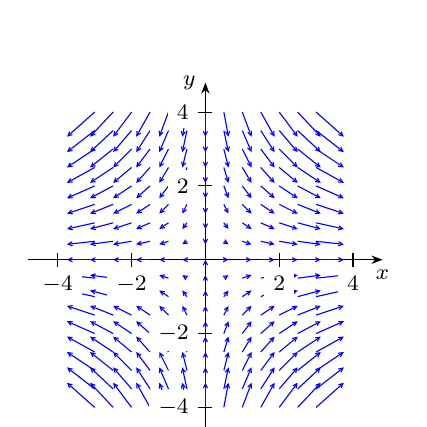
\begin{tikzpicture}[scale=0.46875, baseline=(X.base)]
  \def\scale{0.46875}
  \node at (0,-4) (X) {};

  \drawaxes{-4}{-4}{4}{4}

  \foreach \x in {-3,-2.5,...,3} {
    \foreach \y in {-4,-3.5,...,4} {
      \draw[vector field, shift={(\x,\y)}] (0,0) -- ({\x/4},{-\y/6});
    }
  }

  \drawxlabels{-4/-4, -2/-2, 2/2, 4/4}
  \drawylabels{-4/-4, -2/-2, 2/2, 4/4}
\end{tikzpicture}
&
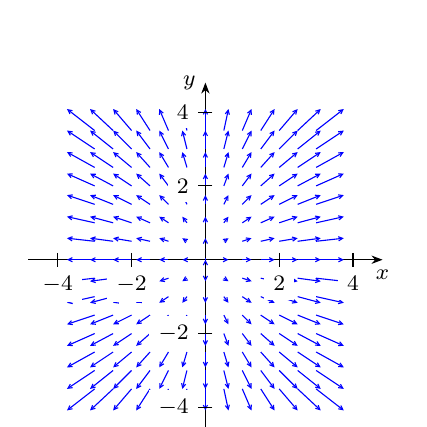
\begin{tikzpicture}[scale=0.46875, baseline=(X.base)]
  \def\scale{0.46875}
  \node at (0,-4) (X) {};

  \drawaxes{-4}{-4}{4}{4}

  \foreach \x in {-3,-2.5,...,3} {
    \foreach \y in {-3.5,-3,...,3.5} {
      \draw[vector field, shift={(\x,\y)}] (0,0) -- ({\x/4},{\y/6});
    }
  }

  \drawxlabels{-4/-4, -2/-2, 2/2, 4/4}
  \drawylabels{-4/-4, -2/-2, 2/2, 4/4}
\end{tikzpicture} \\
(a) & (b)
\end{tabu}
\end{center}
\end{solution}

\begin{question}
Sketch the vector field
\[
\vec\Ph(x,y) = \frac 14 \vec {i} + \frac{1}{9 + x^2+y^2} \vec j
\]
and explain why $\vec\Ph$ is or is not a gradient vector field of a function.
\end{question}

\begin{solution}
The vector field $\vec\Ph$ is not a gradient field. If it were a gradient field, there would exist a function $f(x,y)$ satisfying
\[
f_x(x,y) = \frac 14 \text{ and }
f_y(x,y) = \frac{1}{9+x^2+y^2}\,.
\]
For the mixed partial derivatives we would have $f_{xy} = 0$, but $f_{yx} \neq 0$ and hence such a function cannot exist. A sketch of the vector field can be found below.

\begin{center}
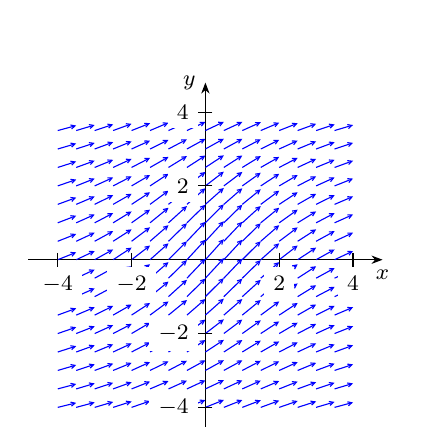
\begin{tikzpicture}[scale=0.46875, baseline=(X.base)]
  \def\scale{0.46875}
  \node at (0,-4) (X) {};

  \drawaxes{-4}{-4}{4}{4}

  \def\factor{5}
  \foreach \x in {-4,-3.5,...,3.5} {
    \foreach \y in {-4,-3.5,...,3.5} {
      \draw[vector field, shift={(\x,\y)}] (0,0) --
        ({\factor*0.1},{\factor/(9+\x*\x+\y*\y)});
    }
  }

  \drawxlabels{-4/-4, -2/-2, 2/2, 4/4}
  \drawylabels{-4/-4, -2/-2, 2/2, 4/4}
\end{tikzpicture}
\end{center}

% \begin{figure}[h]
% \begin{center}
% \includegraphics[width=.4\textwidth]{figures/problems4_2.eps}
% \hspace{0.05\textwidth}
% \includegraphics[width=.4\textwidth]{figures/problems4_3.eps}
% \end{center}
% \caption{Graphs of the vector fields in Problem 2 and Problem 3.}
% \end{figure}
\end{solution}

\begin{question}
For a point $(x,y,z)$ we define the position vector
\[
\vec r = x\vec i + y\vec j + z \vec k
\]
and its length
\[
r = \| \vec r \| = \sqrt{x^2 + y^2+z^2}\,.
\]
\begin{tasks}(2)
\task
Show that $\nabla\left(\frac 1 {r^2}\right) = -\frac{2}{r^4} \vec r$ (for $r\neq 0$).
\task
Find $\nabla\left( \frac 1{r^3} \right)$ (for $r\neq 0$).
\end{tasks}
\end{question}

\begin{solution}
We will solve (a) and (b) at once by finding a formula for the gradient $\nabla \left( \frac{1}{r^\al}\right)$ for any $\al \neq 0$. First we compute the partial derivative
\[
\frac{\p}{\p x} \frac{1}{r^\al} = \frac{\p}{\p x} \left(x^2 + y^2 + z^2\right)^{-\al/2}
= -\frac{\al}2 \left(x^2 + y^2 + z^2 \right)^{-\al/2 - 1} \cdot 2x
= \frac{-\al x}{\left(x^2 + y^2 + z^2 \right)^{\al/2+1}} = -\al \frac{x}{r^{\al+2}}\,.
\]
Since the function $ \frac{1}{r^\al} = \left(x^2 + y^2 + z^2\right)^{-\al/2}$ is symmetric in the variables $x$, $y$ and $z$, we don't need to repeat the calculation for the other derivatives,
\begin{align*}
\frac{\p}{\p x} \frac{1}{r^\al} &= -\al \frac{x}{r^{\al+2}} &
\frac{\p}{\p y} \frac{1}{r^\al} &= -\al \frac{y}{r^{\al+2}} &
\frac{\p}{\p z} \frac{1}{r^\al} &= -\al \frac{z}{r^{\al+2}}\,.
\end{align*}
Therefore the gradient is
\[
\nabla \left(\frac{1}{r^\al}\right)
= -\al \frac{x}{r^{\al+2}} \vec i -\al \frac{y}{r^{\al+2}} \vec j 
-\al \frac{z}{r^{\al+2}} \vec k
= -\al \frac{1}{r^{\al+2}} \left(x \vec i + y \vec j + z \vec k \right)
= -\frac{\al}{r^{\al+2}} \vec r\,.
\]
Now for the specific cases.
\begin{enumerate}
\item
We set $\al =2$ and obtain
\[
\nabla \left( \frac{1}{r^2}\right)
= - \frac{2}{r^{4}} \vec r\,.
\]
\item
We set $\al =3$ and obtain
\[
\nabla \left( \frac{1}{r^3}\right)
= - \frac{3}{r^{5}} \vec r\,.
\]
\end{enumerate}
\end{solution}

\begin{question}
Compute the directional derivatives at the given points in the given directions.
\begin{enumerate}
\item
$f(x,y,z) = x^2 - 2xy + 3z^2$;
$(x_0,y_0,z_0) = (1,1,2)$;
$\vec d = \frac 1{\sqrt{3}} 
\left(\vec i + \vec j - \vec k \right)$.
\item
$f(x,y,z) = \sin\left(xyz\right)$;
$(x_0,y_0,z_0) = \left(1, 1, \frac \pi 4 \right)$;
$\vec d = \left(\frac{\sqrt 2}2, 0, -\frac{\sqrt 2}2\right)$.
\end{enumerate}
\end{question}

\begin{solution}
\begin{enumerate}
\item
The gradient of $f$ is
\[
\nabla f(x,y,z) = (2x-2y) \vec i - 2x \vec j + 6z \vec k\,.
\]
Therefore the directional derivative is
\begin{align*}
\nabla f(1,1,2) \cdot \vec d &= \left( - 2 \vec j + 12 \vec k \right) \cdot
\frac 1{\sqrt{3}} \left(\vec i + \vec j - \vec k \right) \\
&= \frac 1{\sqrt 3} \left( -2 -12 \right) = -\frac{14}{\sqrt 3}\,.
\end{align*}

\item
The gradient of $f$ is
\[
\nabla f(x,y,z) = \cos(xyz) \left( yz \vec i + xz \vec j + xy \vec k \right)\,.
\]
Therefore the directional derivative is
\begin{align*}
\nabla f\left(1, 1, \frac \pi 4 \right) 
&= \frac{\sqrt 2}2 \left(\frac \pi 4 \vec i + \frac \pi 4 \vec j + \vec k \right)
\cdot \frac{\sqrt 2}2 \left(\vec i - \vec k \right) \\
&= \frac 12 \left( \frac \pi 4 - 1 \right) = \frac \pi 8 - \frac 12\,.
\end{align*}
\end{enumerate}
\end{solution}

\begin{question}
Let 
$f(x,y) = \frac{x-y}{x+y}$ and 
$(x_0,y_0) = \left(-\frac 12, \frac 32\right)$. 
Find the directions $\vec u$ and the values of $\nabla f(x_0,y_0) \cdot \vec u$ for which
\begin{tasks}(3)
\task
$\nabla f(x_0,y_0) \cdot \vec u$ is largest
\task
$\nabla f(x_0,y_0) \cdot \vec u$ is smallest
\task
$\nabla f(x_0,y_0) \cdot \vec u = 0$
\task
$\nabla f(x_0,y_0) \cdot \vec u = -2$
\task
$\nabla f(x_0,y_0) \cdot \vec u = 1$
\task
$\nabla f(x_0,y_0) \cdot \vec u = -1$
\end{tasks}
Note that direction vectors have unit length.
\end{question}

\begin{solution}
We have
\[
\nabla f(x,y) = \frac{2y}{(x+y)^2}\vec i + \frac{-2x}{(x+y)^2} \vec j\,,
\qquad
\nabla f\left( -\frac 12, \frac 32\right) = 3 \vec i + \vec j\,.
\]

\begin{enumerate}
\item
From the lectures we know that the directional derivative is maximal in the direction of the gradient. Thus
\[
\vec u = \frac{1}{\sqrt{10}}\left( 3 \vec i + \vec j \right)\,.
\]
Note that we cannot simply set $\vec u = \nabla f\left(-\frac12, \frac 32\right)$, because $\vec u$ has to be a unit vector. Therefore we compute the norm,
\[ \left\| \nabla f\left( -\frac 12, \frac 32\right) \right\|= \sqrt{3^2 + 1} = \sqrt{10} \]
and use the normalized gradient as the direction vector.
\item
Again, the theory tells us that the directional derivative is minimal in the direction opposite to the gradient. Thus
\[
\vec u = -\frac{1}{\sqrt{10}}\left( 3 \vec i + \vec j \right)\,.
\]
\item
The condition $\nabla f(x_0,y_0) \cdot \vec u = 0$ means that $\vec u$ has to be orthogonal to the gradient. In two dimensions it is easy to find these vectors, the two possibilities are
\[
\vec u = \frac{1}{\sqrt{10}}\left( \vec i -3 \vec j \right)\text{ and }
\vec u = -\frac{1}{\sqrt{10}} \left( \vec i -3\vec j \right)\,.
\]
\item
Here we have to do some calculations. Any direction vector $\vec u$ can be written as $\vec u = a\vec i + b\vec j$ with the additional constraint $\| \vec u\|^2 = a^2+b^2 = 1$. Equivalently we can write the constraint as
\[
b = \pm \sqrt{1-a^2}\,.
\]
The condition $\nabla f(x_0,y_0) \cdot \vec u = -2$ is
\begin{align*}
(3\vec i + \vec j) \cdot (a \vec i + b \vec j) &= -2 \\
3a + b &= -2
\end{align*}
and after we substitute for $b$ we get the equation
\[
3a \pm \sqrt{1-a^2} = -2\,.
\]
This equation can be solved as follows
\begin{align*}
3a + 2 &= \mp \sqrt{1-a^2} \\
9a^2 + 12a + 4 &= 1-a^2 \\
10a^2 + 12a + 3 &= 0 \\
a^2 + \frac 65 a + \frac 3{10} &= 0 \\
a &= -\frac 35 \pm \sqrt{ \frac{9}{25} - \frac{3}{10}} \\
a &= \frac{1}{10}\left(-6 \pm \sqrt{6}\right)\,.
\end{align*}
And we get $b$ from the equation
\[
3a + b = -2\,,
\]
leading to
\[
b = -\frac{1}{10} \left( 2 \pm 3 \sqrt{6}\right)\,.
\]
Thus we obtain the two solutions
\begin{align*}
\vec u_1 &= \frac{-6 + \sqrt 6}{10} \vec i - \frac{2 + 3\sqrt 6}{10} \vec j &
\vec u_2 &= \frac{-6 - \sqrt 6}{10} \vec i - \frac{2 - 3\sqrt 6}{10} \vec j
\end{align*}

\item
Following the same strategy as before we arrive at the equation
\begin{align*}
3a \pm \sqrt{1-a^2} &= 1
\end{align*}
Solving it leads to
\begin{align*}
3a-1 &= \mp \sqrt{1-a^2} \\
9a^2 -6a + 1 &= 1 - a^2 \\
10a^2 - 6a &= 0 \\
a(5a-3) &= 0\,.
\end{align*}
This has two solutions: $a=0$ and $a=\frac 35$. Using the equation
\[
3a+b=1\,,
\]
we obtain the two direction vectors
\begin{align*}
\vec u_1 &= \vec j &
\vec u_2 &= \frac 35 \vec i -\frac 45 \vec j\,.
\end{align*}

\item
To answer this question no new calculations are necessary, merely the observation that multiplying the direction by $-1$, changes the sign in the directional derivative, i.e.,
\[
\nabla f(x_0,y_0) \cdot (-\vec u) = - \left( \nabla f(x_0, y_0) \cdot \vec u \right)\,.
\]
Therefore the required direction vectors are
\begin{align*}
\vec u_1 &= -\vec j &
\vec u_2 &= -\frac 35 \vec i +\frac 45 \vec j\,.
\end{align*}
\end{enumerate}
\end{solution}

\begin{question}
The directional derivative of a function $f(x,y,z)$ at some point is greatest in the direction parallel to $\vec i + \vec j - \vec k$. In this direction, the value of the directional derivative is $2\sqrt{3}$.
\begin{enumerate}
\item
What is $\nabla f$ at this point? Give reasons for your answer.
\item
What is the directional derivative of $f$ at the point in the direction $\frac{1}{\sqrt 2}\left(\vec i + \vec j\right)$?
\end{enumerate}
\end{question}

\begin{solution}
\begin{enumerate}
\item
This problem asks us to reconstruct a vector given its direction and magnitude. We know that the directional derivative is greatest in the direction of the gradient. The unit vector representing this direction is
\[
\vec d = \frac{1}{\sqrt{3}} \left( \vec i + \vec j - \vec k \right)\,.
\]
Thus $\vec d$ is the direction of the gradient. Regarding its magnitude, we have the following rule:
\begin{quote}
The directional derivative in the direction of the gradient equals its norm.
\end{quote}
 In other words, if $\vec d$ points along the gradient, then
\[
\nabla f \cdot \vec d = \| \nabla f \|\,.
\]
Why is this the case? If $\vec d$ points in the direction of the gradient, then
\[
\vec d = \frac{1}{\| \nabla f \|} \nabla f\,,
\]
and therefore
\begin{align*}
\nabla f \cdot \vec d &= \nabla f \cdot \frac{1}{\| \nabla f \|} \nabla f
= \frac{1}{\| \nabla f\|} \nabla f \cdot \nabla f
= \frac{1}{\| \nabla f \|} \| \nabla f \|^2
= \| \nabla f \|\,.
\end{align*}
We know the magnitude of the directional derivative and thus the norm of the gradient,
\begin{align*}
\| \nabla f\| &= 2\sqrt{3}\,.
\end{align*}
This allows us to reconstruct $\nabla f$ via
\begin{align*}
\nabla f &= \| \nabla f \| \vec d
= \frac{2\sqrt{3}}{\sqrt{3}} \left( \vec i + \vec j - \vec k \right) \\
&= 2 \left( \vec i + \vec j - \vec k \right)\,.
\end{align*}

\item
The unit vector representing the given direction is
\[
\vec d = \frac{1}{\sqrt{2}} \left( \vec i + \vec j \right) \,,
\]
and the directional derivative is
\[
\nabla f \cdot \vec d = 2 \sqrt{2}\,.
\]
\end{enumerate}
\end{solution}

\begin{question}
Let $f(x,y)$ be a function. At $(1,0)$ the directional derivative in the direction $\frac{1}{\sqrt 5}\left( \vec i + 2 \vec j \right)$ equals $\frac 32$ and in the direction $\frac{1}{\sqrt 5}\left( -2 \vec i + \vec j \right)$ equals $2$. What is the gradient of $f$ at $(1,0)$?
\end{question}

\begin{solution}
We denote the direction vectors by
\begin{align*}
\vec d_1 &= \frac{1}{\sqrt 5}\left( \vec i + 2 \vec j \right) &
\vec d_2 &= \frac{1}{\sqrt 5}\left( -2 \vec i + \vec j \right)\,.
\end{align*}
\begin{wrapfigure}{r}{0.35\textwidth}
\centering
% Directional derivatives from a point in two directions
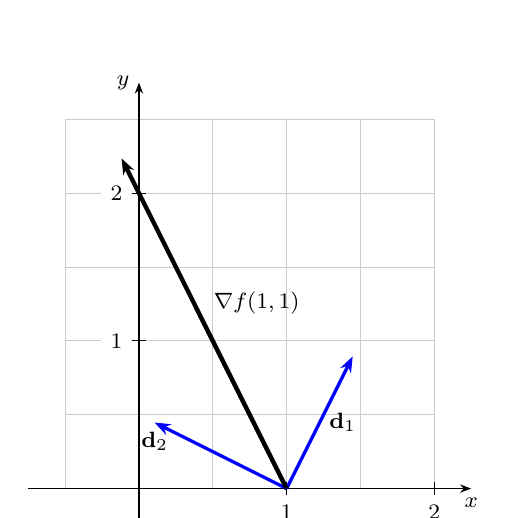
\begin{tikzpicture}[scale=1.875, baseline=(X.base)]
  \def\scale{1.875}
  \draw[coordinate grid, step=0.5] (-0.5,0) grid (2,2.5);
  \node at (0,0) (X) {};

  \drawaxes{-0.5}{0}{2}{2.5}

  \drawxlabels{1/1, 2/2}
  \drawylabels{1/1, 2/2}

  % Directions
  \coordinate (or) at (1,0);

  \coordinate (a) at ($(or)+{1/sqrt(5)}*(1,2)$);
  \coordinate (b) at ($(or)+{1/sqrt(5)}*(-2,1)$);
  \coordinate (c) at ($(or)+({-sqrt(5)/2},{sqrt(5)})$);

  \draw[color=blue,very thick,->] (or) -- (a);
  \node[right] at ($(or)!0.5!(a)$) {$\vec {d}_1$};

  \draw[color=blue,very thick,->] (or) -- (b);
  \node[below] at ($(or)!1!(b)$) {$\vec{d}_2$};

  \draw[ultra thick, ->] (or) -- (c);
  \node[above right] at ($(or)!0.5!(c)$) {$\nabla f(1,1)$};
\end{tikzpicture}
\end{wrapfigure}
The directional derivatives can now be written as
\begin{align*}
\nabla f(1,0) \cdot \vec d_1 &= \frac 32 \\
\nabla f(1,0) \cdot \vec d_2 &= 2\,.
\end{align*}
In coordinates these two equations become
\begin{align*}
f_x + 2f_y &= \frac 32 \sqrt{5} \\
-2f_x + f_y &= 2 \sqrt{5}\,.
\end{align*}
To solve the system we add twice the first equation to the second one and subtract twice the second from the first,
\begin{align*}
5 f_y &= 5 \sqrt{5} \\
5 f_x &= -\frac 52 \sqrt{5}\,.
\end{align*}
And hence the solution is
\[
f_x = -\frac{\sqrt{5}}2 \text{ and } f_y = \sqrt{5}\,.
\]
The gradient is
\[
\nabla f(1,0) = \frac{\sqrt{5}}{2} \left( -\vec i + 2\vec j \right)\,.
\]
\end{solution}

\begin{question}
Let $f(x,y)$ be a function. At $(1,0)$ the directional derivative of $f$ in the direction towards the point $(2,-2)$ equals $0$ and in the direction towards the point $(-1,1)$ equals $1$. What is gradient of $f$?
\end{question}

\begin{solution}
The direction from $(1,0)$ to $(2,-2)$ is
represented by the unit vector
\[
\vec d_1 = \frac 1{\sqrt{5}}\left(\vec i - 2\vec j \right)\,,
\]
\begin{wrapfigure}{r}{0.35\textwidth}
\centering
% Directional derivatives from a point in two directions
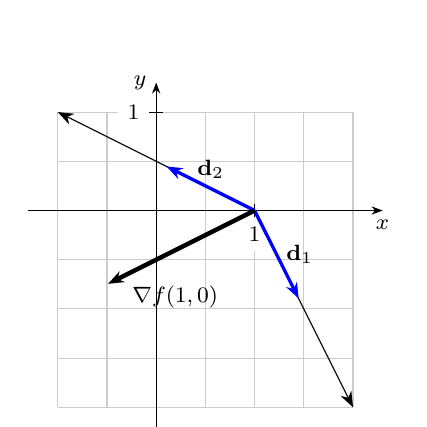
\begin{tikzpicture}[scale=1.25, baseline=(X.base)]
  \def\scale{1.25}
  \draw[coordinate grid, step=.5] (-1,-2) grid (2,1);
  \node at (-1,-2) (X) {};

  \drawaxes{-1}{-2}{2}{1}

  \drawxlabels{1/1}
  \drawylabels{1/1}

  % Directions
  \draw[->] (1,0) -- (2,-2);
  \draw[->] (1,0) -- (-1,1);

  \coordinate (a) at ($(1,0)+{1/sqrt(5)}*(1,-2)$);
  \coordinate (b) at ($(1,0)+{1/sqrt(5)}*(-2,1)$);
  \coordinate (c) at ($(1,0)+{sqrt(5)}*(-0.666,-0.333)$);

  \draw[color=blue,very thick,->] (1,0) -- (a);
  \node[right] at ($(1,0)!0.5!(a)$) {$\vec {d}_1$};

  \draw[color=blue,very thick,->] (1,0) -- (b);
  \node[above] at ($(1,0)!0.5!(b)$) {$\vec{d}_2$};

  \draw[ultra thick, ->] (1,0) -- (c);
  \node[below right] at ($(1,0)!0.9!(c)$) {$\nabla f(1,0)$};
\end{tikzpicture}
\end{wrapfigure}
and the direction from $(1,0)$ to $(-1,1)$ by the unit vector
\[
\vec d_2 = \frac 1{\sqrt{5}}\left(-2 \vec i + \vec j\right)\,.
\]
The directional derivatives can now be written as
\begin{align*}
\nabla f(1,0) \cdot \vec d_1 &= 0 \\
\nabla f(1,0) \cdot \vec d_2 &= 1.
\end{align*}
In coordinates these two equations become
\begin{align*}
f_x - 2f_y &= 0 \\
-2f_x + f_y &= \sqrt{5}\,.
\end{align*}
To solve the system we add twice the first equation to the second one and twice the second one to the first one obtaining
\begin{align*}
- 3f_y &= \sqrt{5} \\
-3f_x  &= 2\sqrt{5}\,.
\end{align*}
Hence the solution is
\[
f_x = -\frac {2\sqrt{5}}{3} \text{ and } f_y = -\frac {\sqrt{5}}{3}\,,
\]
giving the gradient
\[
\nabla f(1,0) = -\frac{\sqrt{5}}{3} \left( 2\vec i + \vec j\right)\,.
\]
\end{solution}

\begin{question}
Let $f(x,y)$ be a function. At $(1,1)$ the directional derivative in the direction towards the point $(2,4)$ equals $2$ and in the direction towards the point $(2,2)$ equals $3$. Find the directional derivative in the direction towards the point $(2,3)$.
\end{question}

\begin{solution}
The direction from $(1,1)$ to $(2,4)$ is represented by the unit vector
\[
\vec{d}_1 = \frac 1{\sqrt{10}} \left(\vec i + 3\vec j\right)\,,
\]
\begin{wrapfigure}{r}{0.35\textwidth}
\centering
% Directional derivatives from a point in two directions
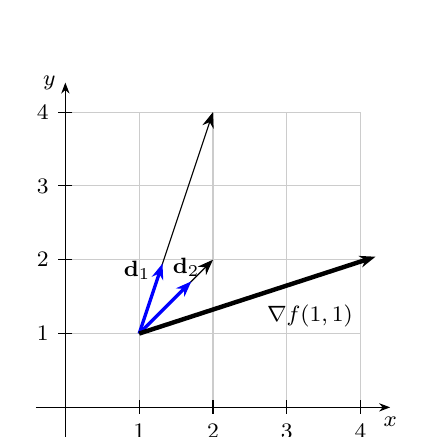
\begin{tikzpicture}[scale=0.9375, baseline=(X.base)]
  \def\scale{0.9375}
  \draw[coordinate grid, step=1] (0,0) grid (4,4);
  \node at (0,0) (X) {};

  \drawaxes{0}{0}{4}{4}

  \drawxlabels{1/1, 2/2, 3/3, 4/4}
  \drawylabels{1/1, 2/2, 3/3, 4/4}

  % Directions
  \coordinate (or) at (1,1);

  \draw[->] (or) -- (2,4);
  \draw[->] (or) -- (2,2);

  \coordinate (a) at ($(or)+{1/sqrt(10)}*(1,3)$);
  \coordinate (b) at ($(or)+{1/sqrt(2)}*(1,1)$);
  \coordinate (c) at ($(or)+({-sqrt(10) + 4.5*sqrt(2)},{sqrt(10)-1.5*sqrt(2)})$);

  \draw[color=blue,very thick,->] (or) -- (a);
  \node[left] at ($(or)!0.9!(a)$) {$\vec {d}_1$};

  \draw[color=blue,very thick,->] (or) -- (b);
  \node[above] at ($(or)!0.9!(b)$) {$\vec{d}_2$};

  \draw[ultra thick, ->] (or) -- (c);
  \node[below right] at ($(or)!0.5!(c)$) {$\nabla f(1,1)$};
\end{tikzpicture}
\end{wrapfigure}
and the direction from $(1,1)$ to $(2,2)$ by the unit vector
\[
\vec{d}_2 = \frac 1{\sqrt{2}} \left(\vec i + \vec j\right)\,,
\]
The directional derivatives can now be written as
\begin{align*}
\nabla f(1,0) \cdot \vec d_1 &= 2 \\
\nabla f(1,0) \cdot \vec d_2 &= 3.
\end{align*}
In coordinates these equations become the following sytem of linear equations
\begin{align*}
f_x + 3f_y &= 2\sqrt{10} \\
f_x + f_y &= 3\sqrt{2}\,,
\end{align*}
where we have omitted the argument $(1,1)$ from $f_x$ and $f_y$. The unique solution of this system is
\begin{align*}
f_x &= -\sqrt{10} + \frac 92 \sqrt{2} &
f_y &= \sqrt{10} - \frac 32 \sqrt{2}\,.
\end{align*}
Thus 
\[
\nabla f(1,1) = \left(-\sqrt{10} + \frac 92 \sqrt{2}\right) \vec i + 
\left(\sqrt{10} - \frac 32 \sqrt{2}\right) \vec j\,.
\]
The direction towards $(2,3)$ is given by the direction vector
\[
\vec{d}_3 = \frac 1{\sqrt{5}} \left( \vec i + 2 \vec j\right)\,,
\]
and the directional derivative is
\[
\nabla f(1,1) \cdot \vec{d}_3 = \sqrt{2} + \frac 3{10} \sqrt{10}\,.
\]
\end{solution}

% \begin{question}
% Let $f(x,y)$ be a function. At $(1,0)$ the directional
% derivative of $f$ towards the point $(3,-3)$ equals $1$
% and the directional derivative towards the point $(-2,2)$
% equals $-4$.

% What is gradient of $f$ at $(1,0)$?

% \hfill[MA2712 Test, January 2015]
% \end{question}

% \begin{solution}
% The direction from $(1,0)$ to $(3,-3)$ is
% represented by the unit vector
% \[
% \vec d_1 = \frac 1{\sqrt{13}}\left(2 \vec i - 3\vec j \right)\,,
% \]
% and the direction from $(1,0)$ to $(-2,2)$ is represented by the unit vector
% \[
% \vec d_2 = \frac 1{\sqrt{13}}\left(-3 \vec i + 2\vec j\right)\,.
% \]
% The directional derivatives can now be written as
% \begin{align*}
% \nabla f(1,0) \cdot \vec d_1 &= 1 \\
% \nabla f(1,0) \cdot \vec d_2 &= -4.
% \end{align*}
% In coordinates these two equations become
% \begin{align*}
% 2f_x - 3f_y &= \sqrt{13} \\
% -3f_x + 2f_y &= -4\sqrt{13}\,.
% \end{align*}
% To solve the system we add and subtract the equations from each other to obtain
% \begin{align*}
% -f_x - f_y &= -3\sqrt{13} \\
% f_x - f_y &= \sqrt{13}
% \end{align*}
% From here we get
% \[
% -2f_y = -2\sqrt{13}
% \]
% and hence the solution is
% \[
% f_x = 2\sqrt{13} \text{ and } f_y = \sqrt{13}\,.
% \]
% The gradient is
% \[
% \nabla f(1,0) = \sqrt{13} \left( 2\vec i + \vec j\right)\,.
% \]
% \end{solution}

\begin{question}
Suppose that a mountain has the shape of an elliptic paraboloid $z = c - ax^2 - by^2$, where $a,b,c$ are positive constants, $x$ and $y$ are the east-west and north-south map coordinates, and $z$ is the altitude above sea level ($x$, $y$ and $z$ are all measured in meters). 
\begin{enumerate}
\item
At the point $(1,1)$, in what direction is the altitude increasing most rapidly? If a marble were released at $(1,1)$, in what direction would it begin to roll?
\item
An engineer wishes to build a railroad up the mountain. Straight up the mountain is much too steep for the power of the engines. At the point $(1,1)$, in what directions may the track be laid so that it will be climbing with a 3\% grade---that is, an angle whose tangent is 0.03. (There are two possibilities.) 
%Make a sketch of the situation indicating the two possible directions for a 3\% grade at $(1,1)$.
\end{enumerate}
\end{question}

\begin{solution}
Denote by $f(x,y) = c - ax^2 - by^2$ the height of the mountain at the point $(x,y)$. 
We have
\[
\nabla f(x,y) = \begin{pmatrix} -2ax \\ -2by \end{pmatrix}
\qquad
\nabla f\left( 1,1 \right) = \begin{pmatrix} -2a \\ -2b \end{pmatrix}\,.
\]

\begin{enumerate}
\item
At the point $(1,1)$ the altitude is increasing most rapidly in the direction of the gradient of $f$, which is
\[
\nabla f(x,y) = -2ax \vec i - 2by \vec j\,.
\]
The gradient at $(1,1)$ is
\[
\nabla f\left( 1,1 \right) = -2a\vec i - 2b \vec j\,.
\]
The direction vector has to have unit length and so
\[
\vec d = -\frac{1}{\sqrt{a^2+b^2}} \left( a \vec i + b \vec j \right)\,,
\]
is the direction of the most rapid increase.

A marble released at this point would roll in the direction of the greatest decrease, which is the direction opposite to $\nabla f$. This direction is described by the vector
\[
-\vec d = \frac{1}{\sqrt{a^2+b^2}} \left( a \vec i + b \vec j \right)\,.
\]

\item
The tangent of an angle is exactly the slope of the corresponding line and we have seen in the lecture, that the slope is given by the directional derivative. This means that we are looking for a direction $\vec d = \la \vec i + \mu \vec j$, where $\la, \mu$ have to be found, such that $\nabla f(1,1) \cdot \vec d = 0.03$, leading to the equation,
\[
-2a\la -2b\mu = 0.03\,.
\]
Now we use that $\la^2 + \mu^2 = 1$ (because $\| \vec d \|=1$) to get the equation
\begin{align*}
2a\sqrt{1-\mu^2} + 2b\mu &= -0.03 \\
a\sqrt{1-\mu^2} &= -(b\mu + 0.015) \\
a^2\left(1-\mu^2\right) &= b^2\mu^2 + 0.03b\mu + 0.015^2 \\
\left(a^2+ b^2\right)\mu^2 + 0.03b\mu + 0.015^2 - a^2 &= 0\,.
\end{align*}
Then we can compute $\la$ from the first equation
\[
\la = -\frac{1}{a}\left( b\mu + 0.015\right)\,.
\]
The two direction vectors then are
\[
\vec d_1 = \frac{1}{a} \begin{pmatrix} -b\mu_1 - 0.015 \\ a\mu_1 \end{pmatrix}
\text{ and }
\vec d_2 = \frac{1}{a} \begin{pmatrix} -b\mu_2 - 0.015 \\ a\mu_2 \end{pmatrix}\,,
\]
where $\mu_1,\mu_2$ are solutions of the quadratic equation
\[
\left(a^2+ b^2\right)\mu^2 + 0.03b\mu + 0.015^2 - a^2 = 0\,.
\]
\end{enumerate}
\end{solution}

%%% Local Variables:
%%% mode: latex
%%% TeX-master: "problems"
%%% End:

\ifthenelse{\boolean{sectionnewpage}}{\newpage}{}
% Version: v1

\section{Gradients and Level Surfaces}
\begin{question}
True or false: $\nabla f(a,b)$ is perpendicular to the graph of $z=f(x,y)$ at the point $(a,b)$?
\end{question}

\begin{solution}
False.

The vector $\nabla f(a,b)$ is perpendicular to the level curves of $f(x,y)$, not to its graph.
\end{solution}

\begin{question}
Find $\nabla f$ at the given point and plot it on the level surface $f(x,y,z)=c$ passing through that point
\begin{tasks}(2)
\task
$f(x,y,z) = x^2 + y^2 + z^2$ at $(0,0,1/2)$
\task
$f(x,y,z) = z - x^2 - y^2$ at $(0,0,1/2)$
\task
$f(x,y,z) = z - x + y$ at $(-1/3,1/3,1/3)$
\task
$f(x,y,z) = x + y - z^2$ at $\left(0,0,0\right)$
\end{tasks}
\end{question}

\begin{solution}
See the figures for plots of the level surfaces.

\begin{center}
\begin{tabu} to \linewidth {X[1,c] X[1,c] X[1,c] X[1,c]}
\asyinclude[width=3.5cm]{asy/level_set_sphere.asy} &
\asyinclude[width=3.5cm]{asy/level_set_paraboloid.asy} &
\asyinclude[width=3.5cm]{asy/level_set_plane.asy} &
\asyinclude[width=3.5cm]{asy/level_set_root.asy} \\
(a) & 
(b) & 
(c) &
(d)
\end{tabu}
\end{center}

The vectors plotted in the figures are the normalized gradients $\frac{1}{\| \nabla f\|} \nabla f$ at the given point.
% \begin{wrapfigure}{r}{4cm}
% \centering
% \asyinclude[width=4cm]{level_set_root.asy}

% (d)
% \end{wrapfigure}

\begin{enumerate}
\item
The level surface 
\[
x^2 + y^2 + z^2 = \frac 12
\] 
is a sphere of radius $\frac{\sqrt{2}}2$ and
$\nabla f\left(0,0,\frac 12\right) = \vec k$.
\item
The level surface 
\[
z = \frac 12 + x^2 + y^2
\]
is a paraboloid, shifted by $\frac 12$ in the $z$-direction and the gradient is
\[
\nabla f\left(0,0,\frac 12\right) = \vec k\,.
\]

\item
The level surface $-x + y + z = 1$ is a plane. To draw it one finds the points, where it crosses the coordinate axes: the $x$-axis at $-1$, the $y$- and $z$-axes at $1$. The gradient is 
\[
\nabla f\left(\frac 13,-\frac 13,\frac 13\right) = -\vec i + \vec j + \vec k\,.
\]

\item
The level surface can be written as the graph of the function $x= z^2 - y$. The gradient is $\nabla f(0,0,0) = \vec i + \vec j$.
\end{enumerate}
\end{solution}

\begin{question}
Find a unit normal to the given surface at the given point.
\begin{tasks}(2)
\task
$xyz=8$ at $(1,1,8)$
\task
$x^2y^2+y-z+1=0$ at $(0,0,1)$
\task
$\cos(xy)= e^z - 2$ at $(1, \pi, 0)$
\task
$e^{xyz} = e$ at $(1,1,1)$
\end{tasks}
\end{question}

\begin{solution}
A normal vector to the surface $f(x,y,z)=c$ at $(x_0,y_0,z_0)$ is given by $\nabla f(x_0,y_0,z_0)$. We obtain a unit normal vector by rescaling the gradient to unit length. Note that there are \emph{two} choices for the unit normal vector, since the vectors $\vec n$ and $-\vec n$ both have the same length.
\begin{enumerate}
\item
With $f(x,y,z) = xyz$ we have
\begin{align*}
\nabla f(x,y,z) &= yz \vec i + xz \vec j + xy \vec k &
\nabla f(1,1,8) &= 8\vec i + 8 \vec j + \vec k\,.
\end{align*}
A unit normal vector is
$\vec n = \frac{1}{\sqrt {129}} \left( 8\vec i + 8 \vec j + \vec k \right)$.

\item
With $f(x,y,z) = x^2y^2 + y -z$ we have
\begin{align*}
\nabla f(x,y,z) &= 2xy^2 \vec i + (2x^2 y + 1) \vec j - \vec k &
\nabla f(0,0,1) &= \vec j - \vec k\,.
\end{align*}
A unit normal vector is 
$\vec n = \frac{1}{\sqrt 2} \left( \vec j - \vec k \right)$.

\item
With $f(x,y,z) = \cos(xy) - e^z$ we have
\begin{align*}
\nabla f(x,y,z) &= -\sin(xy) \left(y \vec i + x \vec j\right) - e^z \vec k &
\nabla f(1,\pi,0) &= -\vec k\,.
\end{align*}
A unit normal vector is $\vec n = \vec k$.

\item
With $f(x,y,z) = e^{xyz}$ we have
\begin{align*}
\nabla f(x,y,z) &= e^{xyz} \left( yz \vec i + xz \vec j + xy \vec k \right) &
\nabla f(1,1,1) &= \vec i + \vec j + \vec k\,.
\end{align*}
A unit normal vector is $\vec n = \frac 1{\sqrt{3}} \left( \vec i + \vec j + \vec k \right)$.
\end{enumerate}
\end{solution}

\begin{question}
Find the equation of the tangent plane to each surface at the indicated point.
\begin{tasks}(2)
\task
$x^2 + y^2 + 3z^2 = 10$; $\left(1, \sqrt{3}, 1\right)$
\task
$xyz^2 = 1$; $(1,1,1)$
\task
$x^2 + 2y^2 + 3xz = 10$; $\left(1, 2, \frac 13\right)$
\task
$y^2 - x^2 = 3$; $(1, 2, 8)$
\end{tasks}
\end{question}

\begin{solution}
The tangent plane to the surface $f(\vec x)=c$ at the point $\vec x_0 = (x_0,y_0,z_0)$ is the plane, which passes through the point $\vec x_0$ and is orthogonal to $\nabla f(\vec x_0)$. The equation of such a plane is
\[
\nabla f(\vec x_0) \cdot (\vec x - \vec x_0) = 0
\quad\Leftrightarrow\quad
f_x(\vec x_0)\cdot(x-x_0) + f_y(\vec x_0)\cdot(y-y_0) + f_z(\vec x_0)\cdot(z-z_0) = 0\,.
\]

\begin{enumerate}
\item
With $f(x,y,z) = x^2+y^2+3z^2$ we have
\begin{align*}
\nabla f(x,y,z) &= 2x \vec i + 2y \vec j + 6z \vec k &
\nabla f\left(1, \sqrt 3, 1 \right) &= 2\vec i + 2\sqrt{3} \vec j + 6 \vec k \,,
\end{align*}
and so the tangent plane has the equation
\begin{align*}
2(x-1) + 2\sqrt{3}(y-\sqrt{3}) + 6(z-1) &= 0 \\
x + \sqrt{3} y + 3z &= 7\,.
\end{align*}

\item
With $f(x,y,z) = xyz^2$ we have
\begin{align*}
\nabla f(x,y,z) &= yz^2 \vec i + xz^2 \vec j + 2xyz \vec k &
\nabla f\left(1, 1, 1 \right) &= \vec i + \vec j + 2 \vec k \,,
\end{align*}
and so the tangent plane has the equation
\begin{align*}
(x-1) + (y-1) + 2(z-1) &= 0 \\
x + y + 2z &= 4\,.
\end{align*}

\item
With $f(x,y,z) = x^2+2y^2+3xz$ we have
\begin{align*}
\nabla f(x,y,z) &= (2x + 3z) \vec i + 4y \vec j + 3x \vec k &
\nabla f\left(1, 2, \frac 13 \right) &= 3\vec i + 8\vec j + 3 \vec k \,,
\end{align*}
and so the tangent plane has the equation
\begin{align*}
3(x-1) + 8(y-2) + 3\left(z-\frac 13\right) &= 0 \\
3x + 8 y + 3z &= 20\,.
\end{align*}

\item
With $f(x,y,z) = y^2 - x^2$ we have
\begin{align*}
\nabla f(x,y,z) &= -2x \vec i + 2y \vec j &
\nabla f\left(1, 2, 8\right) &= -2\vec i + 4\vec j\,,
\end{align*}
and so the tangent plane has the equation
\begin{align*}
-2(x-1) + 4(y-2) + 0\cdot \left(z-8\right) &= 0 \\
-x + 2y &= 3\,.
\end{align*}
\end{enumerate}
\end{solution}

\begin{question}
Suppose that a particle is ejected from the surface $x^2 + y^2 - z^2 = -1$ at the point $\left(1, 1, \sqrt{3}\right)$ in a direction normal to the surface at time $t=0$ with a speed of $10$ units per second. When and where does it cross the $xy$-plane?
\end{question}

\begin{solution}
A normal vector to the surface $x^2+y^2-z^2 = -1$ at the point $\left(1, 1, \sqrt{3}\right)$ is given by $\nabla f\left(1, 1, \sqrt 3\right)$, where $f$ is the function $f(x,y,z) = x^2+y^2-z^2$. The gradient is
\[
\nabla f(x,y,z) = 2x \vec i + 2y \vec j -2z \vec k\,,
\qquad
\nabla f\left(1, 1, \sqrt 3 \right) = 2\vec i + 2 \vec j -2\sqrt{3} \vec k \,.
\]
A unit normal vector is given by
\[
\vec n = \frac{1}{\sqrt{11}}\left( \vec i +  \vec j - \sqrt{3} \vec k \right) \,.
\]
Denote by $\vec r_0 = \left(1, 1, \sqrt 3\right)$ the starting point. Then the path of the particle is described by the curve
\[
\vec \si(t) = \vec r_0 + 10 t \vec n\,,
\]
and we want to know, when this curve crosses the $xy$-plane. It crosses the $xy$-plane, when the $z$-coordinate equals $0$, leading to the equation
\[
\sqrt{3} - \frac{10 \sqrt{3}}{\sqrt{11}} t = 0\,,
\]
which has the solution $t = \displaystyle\frac{\sqrt{11}}{10}$. To find out, where the particle crosses the $xy$-plane, we evaluate
\[
\vec \si\left(\frac{\sqrt{11}}{10}\right) = \left(2, 2, 0 \right)\,.
\]
Thus the particle crosses the $xy$-plane at time $\displaystyle\frac{\sqrt{11}}{10}$ at the point $(2,2,0)$.
\end{solution}

\begin{question}
If $f(x,y) = xy$, find the gradient vector $\nabla f(3,2)$ and use it to find the tangent line to the level curve $f(x,y) = 6$ at the point $(3,2)$. Sketch the level curve, the tangent line, and the gradient vector.
\end{question}

\begin{solution} Even though this function depends only on two variables, instead of three, we can use the
\begin{wrapfigure}{r}{0.35\textwidth}
    \centering
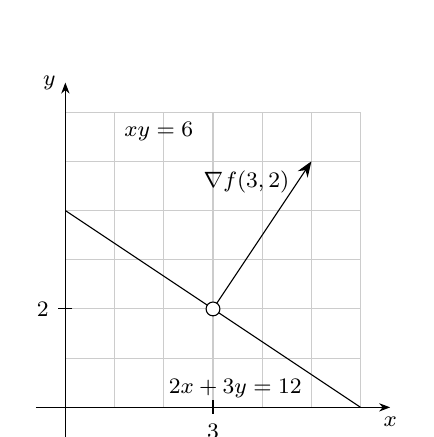
\begin{tikzpicture}[scale=0.625, baseline=(X.base)]
 \def\scale{0.625}

 \draw[coordinate grid, step=1] (0, 0) grid (6, 6);
 \node at (0,0) (X) {};
 \drawaxes{0}{0}{6}{6}

 \drawxlabels[]{3/3}
 \drawylabels[]{2/2}

 \clip (0, 0) rectangle (6, 6);

 \draw[draw=black, domain=1:6, samples=100]
      plot[parametric] function {t, 6/t};

 \draw[draw=black] (0,4) -- (6,0);

 \draw[color=black,->] (3,2) -- (5,5);

 \node[below right] at (1,6) {$xy=6$};
 \node[above left] at (5,0) {$2x+3y=12$};
 \node[below left] at (4.75,5) {$\nabla f(3,2)$};

 \drawpoint{(3,2)};
\end{tikzpicture}
\end{wrapfigure}
same methods to compute the gradient and tangent line. The gradient vector is
\begin{align*}
\nabla f(x,y) &= y\vec i + x \vec j &
\nabla f(3,2) &= 2\vec i + 3 \vec j\,.
\end{align*}
The tangent line is the line through $(3,2)$ that is orthogonal to $\nabla f(3,2)$. It has the equation
\begin{align*}
f_x(3,2)(x-3) + f_y(3,2)(y-2) &= 0 \\
2x + 3y &= 12\,.
\end{align*}
\end{solution}

\begin{question}
At what point on the ellipsoid $x^2 + y^2 + 2z^2 = 1$ is the tangent plane parallel to the plane $x+2y+z=1$?
\end{question}

\begin{solution}
First we compute the tangent plane to the ellipsoid at a general point $(x_0, y_0, z_0)$. The ellipsoid is the level set of $f(x,y,z) = x^2 + y^2 + 2z^2$ for the value 1. Thus
\[
\nabla f(x,y,z) = 2x\vec i + 2y\vec j + 4z\vec k\,,
\]
and the tangent plane is given by
\begin{align*}
2x_0 x + 2y_0 y + 4z_0 z &= 2x_0^2 + 2y_0^2 + 4z_0^2 \\
2x_0 x + 2y_0 y + 4z_0 z &= 2(x_0^2 + y_0^2 + 2z_0^2) \\
x_0 x + y_0 y + 2z_0 z &= 1\,,
\end{align*}
because the point $(x_0,y_0,z_0)$ is assumed to lie on the ellipsoid and thus satisfies $x_0^2 + y_0^2 + 2z_0^2 = 1$.

The question become, for which $(x_0,y_0,z_0)$ are the planes $x_0x + y_0y + 2z_0z = 1$ and $x+2y+z = 1$ parallel. Two planes are parallel, if the normal vectors are parallel. So there must exist $\la \neq 0$, such that
\begin{align*}  
x_0 &= \la &
y_0 &= 2\la &
2z_0 &= \la\,,
\end{align*}
and because $x_0^2 + y_0^2 + 2z_0^2 = 1$, also
\[
\la^2 + 4\la^2 + \frac 12 \la^2 = 1
\quad\Leftrightarrow\quad
\frac {11} 2 \la^2 = 1
\quad\Leftrightarrow\quad
\la = \pm \frac{\sqrt{22}}{11}\,.
\]
Thus we find the two points 
$\left( \frac{\sqrt{22}}{11}, \frac{2\sqrt{22}}{11}, \frac{\sqrt{22}}{22} \right)$
and 
$\left( -\frac{\sqrt{22}}{11}, -\frac{2\sqrt{22}}{11}, -\frac{\sqrt{22}}{22} \right)$.
\end{solution}

\begin{question}
Show that every plane that is tangent to the cone $x^2 + y^2 = z^2$ passes through the origin.
\end{question}

\begin{solution}
The cone is the zero level set of the function $f(x,y,z) = x^2 + y^2 - z^2$, whose gradient is
\[
\nabla f(x,y,z) = 2x\vec i + 2y\vec j - 2z\vec k\,.
\]
The tangent plane at a point $(x_0,y_0,z_0)$ is
\begin{align*}
2x_0x + 2y_0y - 2z_0z &=2x_0^2 + 2y_0^2 - 2z_0^2 \\
x_0 x + y_0 y + z_0z &= 0\,,
\end{align*}
because the point $(x_0,y_0,z_0)$ is assumed to lie on the cone. The right hand side of the equation $x_0 x + y_0 y + z_0z = 0$ vanishes and therefore the tangent plane through $(x_0,y_0,z_0)$ passes through the origin. Since $(x_0,y_0,z_0)$ was an arbitrary point, every tangent plane to the cone passes through the origin.
\end{solution}

\begin{question}
Where does the normal line to the paraboloid $z=x^2 + y^2$ at the point $(1,1,2)$ intersect the paraboloid a second time?
\end{question}

\begin{solution}
The paraboloid is the zero level set of the function $f(x,y,z) = x^2 + y^2 - z$. Its gradient is
\begin{align*}
\nabla f(x,y,z) &= 2x\vec i + 2y\vec j - \vec k &
\nabla f(1,1,2) &= 2\vec i + 2\vec j - \vec k\,.
\end{align*}
The normal line can be parametrized by
\[
\vec \si(t) = \begin{pmatrix} 1 \\ 1 \\ 2 \end{pmatrix}
+ t \begin{pmatrix} 2 \\ 2 \\ -1 \end{pmatrix}
\quad\Leftrightarrow\quad
\vec \si(t) = (1+2t, 1+2t, 2-t)\,.
\]
It intersect the paraboloid, when $f(\vec \si (t)) = 0$, meaning that $t$ satisfies
\begin{align*} 
(1+2t)^2 + (1+2t^2) - (2-t) &= 0 \\
8t^2 + 9t &= 0
\quad\Leftrightarrow\quad
t=0 \text{ or } t = -\frac 98\,.
\end{align*}
When $t=0$ we recover the point $(1,1,2)$ and when $t=-\frac 98$ we find the second point
$\left( -\frac 54, -\frac 54, \frac{25}8 \right)$.
\end{solution}

\begin{question}
Show that the sum of the $x$-, $y$- and $z$-intercepts of any tangent plane to the surface 
$\sqrt x + \sqrt y + \sqrt z = \sqrt c$
is a constant.

\begin{hint*}
The $x$-intercept is where the tangent plane meets the $x$-axis.
\end{hint*}

\begin{solution}
The gradient of the function $f(x,y,z) = \sqrt x + \sqrt y + \sqrt z$ is
\[
\nabla f(x,y,z = \frac 12 \frac 1{\sqrt{x}} \vec i + \frac 12 \frac 1{\sqrt{y}} \vec j
+ \frac 12 \frac 1{\sqrt{z}} \vec k\,,
\]
and the tangent plane at the point $(x_0,y_0,z_0)$ is
\begin{align*}
\frac 12 \frac{x}{\sqrt{x_0}} + \frac 12 \frac{y}{\sqrt{y_0}} 
+ \frac 12 \frac{z}{\sqrt{z_0}} =
\frac 12 \frac{x_0}{\sqrt{x_0}} + \frac 12 \frac{y_0}{\sqrt{y_0}} 
+ \frac 12 \frac{z_0}{\sqrt{z_0}}
\quad\Leftrightarrow\quad
\frac{x}{\sqrt{x_0}} + \frac{y}{\sqrt{y_0}} 
+ \frac{z}{\sqrt{z_0}} = \sqrt c
\end{align*}
What are the intercepts? To find the $x$-intercept, we set $y=z=0$ and obtain $x = \sqrt c \sqrt{x_0}$. Similarly, the $y$-intercept is $y = \sqrt c \sqrt{y_0}$ and the $z$-intercept is $z = \sqrt c \sqrt{z_0}$. Their sum is
\[
\sqrt c \sqrt{x_0} + \sqrt c \sqrt{y_0} + \sqrt c \sqrt{z_0} =
\sqrt c \left(\sqrt{x_0} + \sqrt{y_0} + \sqrt{z_0} \right) = \sqrt c \cdot \sqrt c = c\,,
\]
because the point $(x_0,y_0,z_0)$ satisfies $f(x_0,y_0,z_0) = \sqrt c$. Thus the sum of the intercepts of any tangent plane does not depend on the point, where the tangent plane is computed.
\end{solution}
\end{question}


%%% Local Variables:
%%% TeX-master: "problems"
%%% End:

\ifthenelse{\boolean{sectionnewpage}}{\newpage}{}
% Version: v1

\section{Maxima and Minima}
\begin{question}
True or false: if $(a,b)$ is a critical point of $f(x,y)$, then $(a,b)$ is a local extremum of $f(x,y)$.
\end{question}

\begin{solution}
False.

It is true, that if $(a,b)$ is a local extremum of $f(x,y)$ and the partial derivatives of $f(x,y)$ exist at $(a,b)$, then $(a,b)$ is a critical point of $f(x,y)$. However, the other implication is not true in general, since a critical point can also be a saddle point.
\end{solution}

\begin{question}
True or false: a point $(a,b)$ is a critical point of $f(x,y)$ if $f_x(a,b)=0$ and $f_y(a,b) = 0$.
\end{question}

\begin{solution}
True.

This is the definition of a critical point.
\end{solution}

\begin{question}
True or false: a point $(a,b)$ is a critical point of $f(x,y)$ if $f_x(a,b)$ and $f_y(a,b)$ are undefined.
\end{question}

\begin{solution}
False.

A point is a critical point, if both partial derivatives are defined at the point and equal to $0$.
\end{solution}

\begin{question}
Find the critical points of each of the functions. Decide by inspection whether each of the critical points is a maximum, minimum or a saddle point.
\begin{tasks}(3)
\task
$f(x,y) = x^2+2y^2$
\task
$f(x,y) = x^2-2y^2$
\task
$f(x,y) = e^{-x^2-7y^2+3}$
\end{tasks}
\end{question}

\begin{solution}
\begin{enumerate}
\item
We have
\begin{align*}
f_x &= 2x &
f_y &= 4y\,,
\end{align*}
and hence the only critical point is $(0,0)$. We have $f(0,0) = 0$ and because
\[
f(x,y) = x^2 + 2y^2 \geq 0\,,
\]
we have the inequality $f(x,y) \geq f(0,0)$ for all points $(x,y)$. Thus $(0,0)$ is a global minimum.
\item
We have
\begin{align*}
f_x &= 2x &
f_y &= -4y\,,
\end{align*}
and hence the only critical point is $(0,0)$ with $f(0,0) = 0$. We note however that for $x \neq 0$ we have $f(x,0) =x^2 > 0$, while for $y \neq 0$ we have $f(y,0) = -2y^2 < 0$. In particular $f(1,0) > f(0,0)$, while $f(0,1) < f(0,0)$. Thus $(0,0)$ is neither a maximum nor a minimum; hence it has to be a saddle point.
\item
We have
\begin{align*}
f_x &= -2x e^{-x^2-7y^2+3} &
f_y &= -14y e^{-x^2-7y^2+3}\,,
\end{align*}
and hence the only critical point is $(0,0)$ with $f(0,0) = e^3$. Since $-x^2 -7^2 \leq 0$, we have
\[
f(x,y) = e^{-x^2-7y^2+3} = e^{-x^2-7y^2} \cdot e^3 \leq e^3 = f(0,0)\,.
\]
This implies that the point $(0,0)$ is a global maximum.
\end{enumerate}
\end{solution}

\begin{question}
Use the maximum-minimum test for quadratic functions to decide whether $(0,0)$ is a maximum, minimum or a saddle point.
\begin{tasks}(2)
\task
$f(x,y) = x^2+xy+y^2$
\task
$f(x,y) = y^2-x^2+3xy$
\task
$f(x,y) = 3+2x^2-xy+y^2$
\task
$f(x,y) = 1-x^2+2xy-6y^2$
\end{tasks}
\end{question}

\begin{solution}
Note that the general form of a quadratic function is
\[
g(x,y) = Ax^2 + 2B xy + C y^2\,;
\]
pay particular attention to the factor $2$ in $2B$.
\begin{enumerate}
\item
$A=1$, $B=\frac 12$, $C=1$. We have
$A > 0$ and $AC-B^2= \frac 34 > 0$
and thus $(0,0)$ is a minimum.

\item
$A=-1$, $B=\frac 32$, $C=1$. We have 
$AC-B^2 = -\frac {13}4 < 0$ 
and thus $(0,0)$ is a saddle point.

\item
$A=2$, $B=-\frac 12$, $C=1$. We have 
$A > 0$ and $AC-B^2 = \frac {7}4 > 0$
and thus $(0,0)$ is a minimum.

\item
$A=-1$, $B = 1$, $C=-6$. We have
$A < 0$ and $AC-B^2 = 1 > 0$
and thus $(0,0)$ is a maximum.
\end{enumerate}
\end{solution}

\begin{question}
Explain, why the maximum-minimum test for quadratic functions is a special case of the second derivative test.
\end{question}

\begin{solution}
Consider the quadratic function
\[
g(x,y) = Ax^2 + 2Bxy + Cy^2\,.
\]
The only critical point is $(0,0)$ and the second derivatives of $g(x,y)$ are
\begin{align*}
g_{xx} &= 2A &
g_{xy} &= 2B &
g_{yy} &= 2C\,.
\end{align*}
The second derivative test states that if at $(0,0)$ we have $g_{xx} < 0$ and $g_{xx}g_{yy} - g_{xy}^2 > 0$, then $(0,0)$ is a local minimum. For our function $g(x,y)$ this means
\[
2A < 0 \text{ and } 4AC - 4B^2 > 0\,.
\]
When we divive the first inequality by $2$ and the second one by $4$, we recover the maximum-minimum test for quadratic functions. The same argument can be used for the other types of critical points.

\begin{note*}
There is one slight difference between the two tests though. The second derivative test tells us when a critical point is a \emph{local} maximum or minimum. For a quadratic function it is true that a local maximum or minimum is in fact a \emph{global} one.
\end{note*}
\end{solution}

\begin{question}
Find the critical points of the following functions and classify them using the second derivative test.
\begin{tasks}(2)
\task
$f(x,y) = 2x^2-2xy+y^2-2x+1$
\task
$f(x,y) = x^3 + 3xy + y^3$
\task
$f(x,y) = 5 + 3x^2 + x^3 + 3y^2$
\task
$f(x,y) = x^3 - 2x^2 - 4y^2$
\task
$f(x,y) = -1 + 2x^2 - \frac 12 y^2 + y^4 + 2x^3$
\task
$f(x,y) = \frac 1x + xy + \frac 1y$
\end{tasks}
\end{question}

\begin{solution}
\begin{enumerate}
\item
The partial derivatives of $f(x,y)$ are
\begin{align*}
f_x(x,y) &= 4x - 2y - 2 &
f_y(x,y) &= -2x + 2y\,.
\end{align*}
Critical point are solutions to the equations
\begin{align*}
4x - 2y - 2 &= 0 \\
-2x + 2y &= 0\,.
\end{align*}
The second equation gives $x=y$ and the first equation leads to $y=1$. Thus the only critical point is $(1,1)$. To determine the type of the critical point we compute
\begin{align*}
f_{xx}(x,y) &= 4 &
f_{xy}(x,y) &= -2 &
f_{yy}(x,y) &= 2\,,
\end{align*}
and so
\begin{center}
%\renewcommand{\arraystretch}{1.25}
\begin{tabular}{c|ccc|cc}
 & $A$ & $B$ & $C$ & $AC-B^2$ & Type \\ \hline
$\left(1, 1\right)$ & $4$ & $-2$ & $2$ & $4$ & Local minimum
\end{tabular}
\end{center}

\item
The partial derivatives of $f(x,y)$ are
\begin{align*}
f_x &= 3x^2+3y &
f_y &= 3x+3y^2\,.
\end{align*}
Critical points are solutions to the equations
\begin{align*}
x^2+y &= 0 \\
x+y^2 &=0\,.
\end{align*}
We use the first equation to substitute $y=-x^2$ into the second equation to obtain
\[
x+x^4 = 0\,.
\]
This can be factorized into $x(1+x^3) =0$ leading to two solutions $x=0$ and $x=-1$. Thus we obtain the two critical points $(0,0)$ and $(-1,-1)$. To determine their type we compute
\begin{align*}
f_{xx} &= 6x &
f_{xy} &= 3 &
f_{yy} &= 6y\,.
\end{align*}
Evaluated at the critical points we get
\begin{center}
%\renewcommand{\arraystretch}{1.25}
\begin{tabular}{c|ccc|cc}
 & $A$ & $B$ & $C$ & $AC-B^2$ & Type \\ \hline
$\left(0, 0\right)$ & $0$ & $3$ & $0$ & $-9$ & Saddle point \\
$\left(-1, -1\right)$ & $6$ & $3$ & $6$ & $27$ & Local minimum
\end{tabular}
\end{center}

\item
The partial derivatives of $f(x,y)$ are
\begin{align*}
f_x &= 6x + 3x^2 &
f_y &= 6y\,.
\end{align*}
Critical points are solutions of
\begin{align*}
2x + x^2 &= 0 \\
y &=0\,.
\end{align*}
We have two critical points at $(0,0)$ and $(-2,0)$. To determine their type we compute
\begin{align*}
f_{xx} &= 6+6x &
f_{xy} &= 0 &
f_{yy} &= 6 \,.
\end{align*}
Thus we have
\begin{center}
%\renewcommand{\arraystretch}{1.25}
\begin{tabular}{c|ccc|cc}
 & $A$ & $B$ & $C$ & $AC-B^2$ & Type \\ \hline
$\left(0, 0\right)$ & $6$ & $0$ & $6$ & $36$ & Local minimum \\
$\left(-2, 0 \right)$ & $-6$ & $0$ & $6$ & $-36$ &  Saddle point \\
\end{tabular}
\end{center}

\item
The partial derivatives of $f(x,y)$ are
\begin{align*}
f_x &= 3x^2 - 4x &
f_y &= -8y\,.
\end{align*}
Critical points are solutions of
\begin{align*}
3x^2 -4x &= 0 \\
y &=0\,.
\end{align*}
We have two critical points at $(0,0)$ and $\left(\frac 43,0\right)$. To determine their type we compute
\begin{align*}
f_{xx} &= 6x-4 &
f_{xy} &= 0 &
f_{yy} &= -8 \,.
\end{align*}
Thus we have
\begin{center}
%\renewcommand{\arraystretch}{1.25}
\begin{tabular}{c|ccc|cc}
 & $A$ & $B$ & $C$ & $AC-B^2$ & Type \\ \hline
$\left(0, 0\right)$ & $-4$ & $0$ & $-8$ & $32$ & Local maximum \\
$\left(4/3, 0 \right)$ & $4$ & $0$ & $-8$ & $-32$ &  Saddle point \\
\end{tabular}
\end{center}

\item
The partial derivatives of $f(x,y)$ are
\begin{align*}
f_x &= 4x + 6x^2 &
f_y &= -y + 4y^3\,.
\end{align*}
Critical points are solutions of
\[
\begin{aligned}
2x + 3x^2 &= 0 \\
-y + 4y^3 &=0
\end{aligned}
\quad\Leftrightarrow\quad
\begin{aligned}
x(2+3x) &= 0 \\
y(4y^2-1) &= 0\,.
\end{aligned}
\]
We have six solutions $(0,0)$, $\left(0,\frac 12\right)$, $\left(0,-\frac 12\right)$, $\left(-\frac 23,0\right)$, $\left(-\frac 23,\frac 12\right)$, $\left(-\frac 23,-\frac 12\right)$.
To determine their type we compute
\begin{align*}
f_{xx} &= 4 + 12x &
f_{xy} &= 0 &
f_{yy} &= -1 + 12y^2\,.
\end{align*}
Thus we have
\begin{center}
%\renewcommand{\arraystretch}{1.25}
\begin{tabular}{c|ccc|cc}
 & $A$ & $B$ & $C$ & $AC-B^2$ & Type \\ \hline
$\left(0, 0\right)$ & $4$ & $0$ & $-1$ & $-4$ &  Saddle point \\
$\left(0, \pm 1/2 \right)$ & $4$ & $0$ & $2$ & $8$ & Local minimum \\
$\left(-2/3, 0 \right)$ & $-4$ & $0$ & $-1$ & $4$ & Local maximum\\
$\left(-2/3, \pm 1/2 \right)$ & $-4$ & $0$ & $2$ & $-8$ & Saddle point
\end{tabular}
\end{center}

\item
The partial derivatives of $f(x,y)$ are
\begin{align*}
f_x &= -\frac 1{x^2} + y & 
f_y &= x - \frac{1}{y^2}\,.
\end{align*}
Critical points are solutions of
\begin{align*}
-\frac 1{x^2} + y &= 0 \\
x - \frac{1}{y^2} &=0\,.
\end{align*}
The only critical point is $(1,1)$. To determine its type we compute
\begin{align*}
f_{xx} &= \frac{2}{x^3} &
f_{xy} &= 1 &
f_{yy} &= \frac{2}{y^3}\,.
\end{align*}
Evaluated at $(1,1)$ we get
\begin{center}
%\renewcommand{\arraystretch}{1.25}
\begin{tabular}{c|ccc|cc}
 & $A$ & $B$ & $C$ & $AC-B^2$ & Type \\ \hline
$\left(1, 1 \right)$ & $2$ & $1$ & $2$ & $3$ & Local minimum
\end{tabular}
\end{center}
\end{enumerate}
\end{solution}

\begin{question}
Find and classify the critical points of the following functions.
\begin{tasks}(2)
\task
$f(x,y) = x^3+3xy^2-15x+y^3-15y$
\task
$f(x,y) = (x^2+y^2)e^{x^2-y^2}$
\task
$f(x,y) = \ln(ax^2 + by^2 + 1)$ with $a,b > 0$
\task
$f(x,y) = \frac{x^3-3x}{1+y^2}$
\end{tasks}
\end{question}

\begin{solution}
\begin{enumerate}
\item
The partial derivatives of $f(x,y)$ are
\begin{align*}
f_x(x,y) &= 3x^2+3y^2-15 &
f_y(x,y) = 6xy+3y^2-15 \,.
\end{align*}
Critical point are solutions to the equations
\begin{align*}
3x^2+3y^2-15 &= 0 \\
6xy+3y^2-15 &= 0\,.
\end{align*}
We subtract the second equation from the first to obtain
\[
3x^2 - 6xy = 0
\quad\Leftrightarrow\quad
3x \left(x-2y\right) = 0\,.
\]
We have two cases two consider.
\begin{itemize}
\item
If $x=0$, then the first equation gives
\[
3y^2 - 15 = 0\;\Rightarrow\; y = \pm \sqrt{5}\,,
\]
leading to the two critical points $\left(0, \sqrt 5\right)$ and $\left(0, -\sqrt 5\right)$.
\item
If $x=2y$, then the first equation becomes
\[
15y^2 = 15\;\Rightarrow\; y = \pm 1\,,
\]
leading to two more critical points $(1, 2)$ and $-1, -2)$.
\end{itemize}
To determine the type of the critical points we need the second derivatives
\begin{align*}
f_{xx}(x,y) &= 6x &
f_{xy}(x,y) &= 6y &
f_{yy}(x,y) &= 6x+6y\,.
\end{align*}
Thus we have
\begin{center}
\renewcommand{\arraystretch}{1.25}
\begin{tabular}{c|ccc|cc}
 & $A$ & $B$ & $C$ & $AC-B^2$ & Type \\ \hline
$\left(0, \sqrt 5\right)$ & $0$ & $6\sqrt{5}$ & $6\sqrt{5}$ & $-180$ & Saddle point \\
$\left(0, -\sqrt 5\right)$ &  $0$ & $-6\sqrt{5}$ & $-6\sqrt{5}$ & $-180$ & Saddle point \\
$\left(2,1 \right)$ &  $12$ & $6$ & $18$ & $180$ & Local minimum \\
$\left(-2,-1 \right)$ &  $-12$ & $-6$ & $-18$ & $180$ & Local maxmimum \\
\end{tabular}
\end{center}

\item
The partial derivatives of $f(x,y)$ are
\begin{align*}
f_x(x,y) &= e^{x^2-y^2} \left( 2x + 2x\left(x^2 + y^2\right)\right) &
f_y(x,y) &= e^{x^2-y^2} \left( 2y - 2y\left(x^2 + y^2\right)\right) \,.
\end{align*}
Critical point are solutions to the equations
\begin{align*}
e^{x^2-y^2} \left( 2x + 2x\left(x^2 + y^2\right)\right) &= 0\\
e^{x^2-y^2} \left( 2y - 2y\left(x^2 + y^2\right)\right) &= 0 \,.
\end{align*}
This system is equivalent to
\begin{align*}
2x\left(x^2 + y^2 + 1 \right) &= 0\\
2y\left(x^2 + y^2 - 1 \right) &= 0 \,.
\end{align*}
In the first equation we see that $x^2 + y^2 + 1 \neq 0$ and so $x=0$. From the second equation we obtain
\[
y=0 \text{ or } x^2 + y^2 = 1\,.
\]
This leads to the three solutions $(0,0)$, $(0,1)$ and $(0,-1)$.

To determine the type of the critical points we need the second derivatives
\begin{align*}
f_{xx}(x,y) &= e^{x^2-y^2}\left(2 + 6x^2 + 2y^2 + 4x^2 + 4x^2\left(x^2 + y^2\right)\right) \\
f_{xy}(x,y) &= e^{x^2-y^2}\left(4xy - 4xy - 4xy\left(x^2 + y^2\right)\right) \\
f_{yy}(x,y) &= e^{x^2-y^2}\left(2 - 2x^2 - 6y^2 - 4y^2 + 4y^2 \left(x^2 + y^2\right)\right)
\end{align*}
Thus we have
\begin{center}
\renewcommand{\arraystretch}{1.25}
\begin{tabular}{c|ccc|cc}
 & $A$ & $B$ & $C$ & $AC-B^2$ & Type \\ \hline
$\left(0, 0\right)$ & $2$ & $0$ & $2$ & $4$ & Local minimum \\
$\left(0, 1\right)$ &  $4e^{-1}$ & $0$ & $-4e^{-1}$ & $-16e^{-2}$ & Saddle point \\
$\left(0, -1\right)$ &  $4e^{-1}$ & $0$ & $-4e^{-1}$ & $-16e^{-2}$ & Saddle point
\end{tabular}
\end{center}

\item
The partial derivatives of $f(x,y)$ are
\begin{align*}
f_x(x,y) &= \frac{2ax}{ax^2 + by^2 + 1} &
f_y(x,y) &= \frac{2by}{ax^2 + by^2 + 1} \,.
\end{align*}
Critical point are solutions to the equations
\begin{align*}
\frac{2ax}{ax^2 + by^2 + 1} &= 0 \\
\frac{2ay}{ax^2 + by^2 + 1} &= 0\,.
\end{align*}
Because $ax^2 + by^2 + 1 \neq 0$, the only critical point is $(0,0)$. To determine the type of the critical point we need the second derivatives
\begin{align*}
f_{xx}(x,y) &= \frac{2a}{ax^2 + by^2 + 1} - \frac{4a^2x^2}{\left(ax^2 + by^2 + 1\right)^2}\\
f_{xy}(x,y) &= - \frac{4abxy}{\left(ax^2 + by^2 + 1\right)^2}\\
f_{yy}(x,y) &= \frac{2b}{ax^2 + by^2 + 1} - \frac{4b^2y^2}{\left(ax^2 + by^2 + 1\right)^2}
\end{align*}
Thus we have
\begin{center}
\renewcommand{\arraystretch}{1.25}
\begin{tabular}{c|ccc|cc}
 & $A$ & $B$ & $C$ & $AC-B^2$ & Type \\ \hline
$\left(0, 0\right)$ & $2a$ & $0$ & $2b$ & $4ab > 0$ & Local minimum
\end{tabular}
\end{center}

\item
The partial derivatives of $f(x,y)$ are
\begin{align*}
f_x(x,y) &= \frac{3x^2-3}{1+y^2} &
f_y(x,y) &= -2y \frac{x^3-3x}{\left(1+y^2\right)^2} \,.
\end{align*}
Critical point are solutions to the equations
\begin{align*}
\frac{3x^2-3}{1+y^2} &= 0 \\
-2y \frac{x^3-3x}{\left(1+y^2\right)^2} &= 0\,.
\end{align*}
We can multiply both equations by $(1+y^2)$ and $\left(1+y^2\right)^2$ respectively to obtain
\begin{align*}
3\left(x^2 - 1\right) &= 0\;\Rightarrow\; x = \pm 1 \\
-2xy\left(x^2 - 3 \right) &= 0\;\Rightarrow\; y = 0 \text{ or }x = 0 \text{ or } x = \pm \sqrt{3}\,.
\end{align*}
Note however that since the first equation specifies $x= \pm 1$, it follows that we have $y=0$, because the other cases in the second equation cannot happen. Thus we have the two critical points $(1,0)$ and $(-1,0)$. To determine the type of the critical points we need the second derivatives
\begin{align*}
f_{xx}(x,y) &= \frac{6x}{1+y^2}\\
f_{xy}(x,y) &= -2y \frac{3x-3}{\left(1 + y^2\right)^2}\\
f_{yy}(x,y) &= -2\frac{x^3-3x}{\left(1+y^2\right)^2} +8y^2 \frac{x^3-3x}{\left(1+y^2\right)^3}
\end{align*}
Thus we have
\begin{center}
\renewcommand{\arraystretch}{1.25}
\begin{tabular}{c|ccc|cc}
 & $A$ & $B$ & $C$ & $AC-B^2$ & Type \\ \hline
$\left(1, 0\right)$ & $6$ & $0$ & $4$ & $24$ & Local minimum \\
$\left(-1, 0\right)$ & $-6$ & $0$ & $-4$ & $24$ & Local maximum
\end{tabular}
\end{center}
\end{enumerate}
\end{solution}

\begin{question}
Find the point on the plane $x+2y+3z-10=0$, that minimizes the distance
\begin{tasks}(2)
\task
to the origin;
\task
to the point $(1,1,1)$.
\end{tasks}

\begin{hint*}
Minimize the squared distance to simplify calculations.
\end{hint*}
\end{question}

\begin{solution}
\begin{enumerate}
\item
It is easiest to express each point on the plane in the form
\[
(10-2y-3z, y, z) \text{ with } (y,z) \text{ a point in the $yz$-plane.}
\]
The function we want to minimize is the squared distance
\[
f(y,z) = (10-2y-3z)^2 + y^2 + z^2\,.
\]
Critical points are solutions of
\begin{align*}
2y - 4(10-2y-3z) &= 0 \\
2z - 6 (10-2y-3z) &= 0\,.
\end{align*}
The only solution is $\displaystyle y=\frac{10}7$, $\displaystyle z=\frac{15}7$. The corresponding $x$-coordinate is
\[
x = 10-2\frac {10}7 -3\frac{15}7 = \frac 5 7\,.
\]
Hence the point on the plane, closest to the origin, is $\displaystyle \left(\frac 57, \frac{10}7, \frac{15}7 \right)$.

\item
In this case the function we want to minimize is
\[
f(y,z) = (10-2y-3z-1)^2 + (y-1)^2 + (z-1)^2\,.
\]
Critical points are solutions of
\begin{align*}
2y-2 - 4(9-2y-3z) &= 0 \\
2z-2 - 6 (9-2y-3z) &= 0\,.
\end{align*}
The only solution is $\displaystyle y=\frac{11}7$, $\displaystyle z=\frac{13}7$. The corresponding $x$-coordinate is
\[
x = 10-2\frac {11}7 -3\frac{13}7 = \frac 9 7\,.
\]
Hence the point on the plane, closest to $(1,1,1)$, is $\displaystyle \left(\frac 97, \frac{11}7, \frac{13}7 \right)$.
\end{enumerate}
\end{solution}

\begin{question}
Let $f(x,y) > 0$ for all $x$, $y$. Show that the functions $f(x,y)$ and $g(x,y) = [f(x,y)]^2$ have the same critical points with the same type (local maximum, minimum or saddle point).
\end{question}

\begin{solution}
The partial derivatives of $g(x,y)$ are
\begin{align*}
g_x(x,y) &= 2f(x,y)f_x(x,y) &
g_y(x,y) &= 2f(x,y)f_y(x,y) \,.
\end{align*}
The critical points of $g(x,y)$ are solutions of
\begin{align*}
2f(x,y)f_x(x,y) &= 0 \\
2f(x,y)f_y(x,y) &= 0\,.
\end{align*}
Since we assume that $f(x,y) > 0$, we can divide both equations by $2f(x,y)$. Thus $(a,b)$ is a solution to the above system of equations if and only if $f_x(a,b) = 0$ and $f_y(a,b) =0$. In other words, $(a,b)$ is a critical point of $g(x,y)$ if and only if it is a critical point of $f(x,y)$.

Let us consider the type of the critical point. The second partial derivatives of $g(x,y)$ are
\begin{align*}
g_{xx}(x,y) &= 2f_x(x,y)^2 + 2f(x,y)f_{xx}(x,y) \\
g_{xy}(x,y) &= 2f_x(x,y)f_y(x,y) + 2f(x,y)f_{xy}(x,y) \\
g_{yy}(x,y) &= 2f_y(x,y)^2 + 2f(x,y)f_{yy}(x,y)\,.
\end{align*}
However, at a critical point $(a,b)$ they simplify to
\begin{align*}
g_{xx}(a,b) &= 2f(a,b)f_{xx}(a,b) &
g_{xx}(a,b) &= 2f(a,b)f_{xy}(a,b) &
g_{xx}(a,b) &= 2f(a,b)f_{yy}(a,b)\,.
\end{align*}
Because $f(a,b) > 0$, we see that $g_{xx}(a,b)$ and $f_{xx}(a,b)$ have the same sign, and because at a critical point
\[
g_{xx}g_{yy} - g_{xy}^2 = 4f^2 (f_{xx}f_{yy} - f_{xy}^2)\,,
\]
also the signs of $g_{xx}g_{yy} - g_{xy}^2$ and $f_{xx}f_{yy} - f_{xy}^2$ coincide at $(a,b)$. Therefore the type of $(a,b)$ as a critical point of $f(x,y)$ is the same as a critical point of $g(x,y)$.

\begin{note*}
How would the result change, if we assumed $f(x,y) < 0$ for all $x$, $y$ instead?
\end{note*}
\end{solution}

\begin{question}
For which values of $k$ does
\[
f(x,y) = x^2 + kxy + 4y^2
\]
have a local minimum at $(0,0)$?
\end{question}

\begin{solution}
To study the type of a critical point we look at second derivatives.
\begin{align*}
f_{xx} &= 2 &
f_{xy} &= k &
f_{yy} &= 8\,.
\end{align*}
We see that $(0,0)$ is a minimum, when $16-k^2 > 0$ or equivalently $|k| < 4$. When $|k| > 4$, the point $(0,0)$ is a saddle point.

What happens for $k=\pm 4$? Then the second derivative test is inconclusive and we have to take a closer look at the function. We have
\[
f(x,y) = x^2 \pm 4xy + 4y^2 = (x \pm 2y)^2 \geq 0\,.
\]
Thus $(0,0)$ is a minimum for $k =\pm 4$.
\end{solution}

\begin{question}
Find two numbers $a$ and $b$, such that
\[
\int_a^b (6-x-x^2) \ud x
\]
has its largest value.
\end{question}

\begin{solution}
The problem asks us to find the interval $[a,b]$, that maximizes the value of the integral
\begin{wrapfigure}{r}{0.35\textwidth}
    \centering
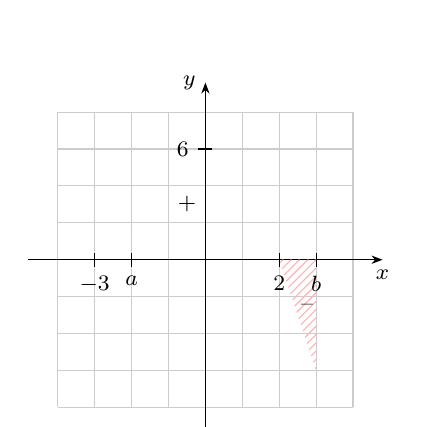
\begin{tikzpicture}[scale=0.46875, baseline=(X.base)]
 \def\scale{0.46875}

 \draw[coordinate grid, step=1] (-4, -4) grid (4, 4);
 \node at (0,-2) (X) {};
 \drawaxes{-4}{-4}{4}{4}

 \clip (-4, -4) rectangle (4, 4);

 \fill[pattern=north east lines, pattern color=blue!30] 
   (-2, 0) -- (-2, 2)
   -- plot[parametric, domain={-2:2}, samples=100] 
        function {t, 0.5*(6-t-t**2)}
   -- (-2, 0);

 \fill[pattern=north east lines, pattern color=red!30] 
   (2, 0) -- (3, 0) -- (3,-3)
   -- plot[parametric, domain={3:2}, samples=100] 
        function {t, 0.5*(6-t-t**2)} -- (2,0);

 \draw[draw=black, domain=-4:4, samples=100]
      plot[parametric] function {t, 0.5*(6-t-t**2)};

 \drawxlabels[]{-3/-3, -2/a, 2/2, 3/b}
 \drawylabels[]{3/6}

 \node at (-0.5,1.5) {+};
 \node at (2.75,-1.25) {--};
\end{tikzpicture}
\end{wrapfigure}
\[
\int_a^b (6-x-x^2) \ud x\,.
\]
Because the integral computes the \emph{signed} area between the graph of a function and the $x$-axis, it is clear from the figure that the integral is maximal for $a=-3$ and $b=2$, which are the two roots of the polynomial $6-x-x^2$.

We can check our result using multivariable calculus. Consider the function
\[
F(a,b) = \int_a^b (6-x-x^2) \ud x\,.
\]
Its partial derivatives are
\begin{align*}
F_a(a,b) &= -(6-a-a^2) &
F_b(a,b) &= 6-b-b^2\,,
\end{align*}
and we see that $(-3,2)$ is indeed a critical point of $F(a,b)$.
\end{solution}

\begin{question}
The discriminant $f_{xx}f_{yy} - f_{xy}^2$ is $0$ at the origin for each of the following functions, so the second derivative test fails to determine the type of the critical point. Determine whether the function has a local maximum, minimum, or neither at the origin by imagining what the surface $z=f(x,y)$ looks like. Briefly justify your reasoning in each case.
\begin{tasks}(2)
\task
$f(x,y) = x^2y^2$
\task
$f(x,y) = 1 - x^2y^2$
\task
$f(x,y) = xy^2$
\task
$f(x,y) = x^3y^3$
\end{tasks}
\end{question}

\begin{solution}
\begin{enumerate}
\item
We have $f(0,0) = 0$ and $f(x,y) = x^2y^2 \geq 0$ for all $x$, $y$. Therefore $(0,0)$ is a minimum.
\item
We have $f(0,0) = 1$ and 
\[
f(x,y) = 1 - x^2y^2 \leq 1
\]
for all $x$, $y$. Therefore $(0,0)$ is a maximum.
\item
We have $f(0,0) = 0$. If $x > 0$ and $y \neq 0$, then $f(x,y) > 0$, while for $x < 0$ and $y \neq 0$ we have $f(x,y) < 0$. Thus $(0,0)$ is a saddle point.
\item
We have $f(0,0) = 0$. If $x > 0$ and $y > 0$, then $f(x,y) > 0$, while for $x > 0$ and $y < 0$ we have $f(x,y) < 0$. Thus $(0,0)$ is a saddle point.
\end{enumerate}
\end{solution}


\begin{question}
Consider the general problem of finding the points on a graph $z = g(x,y)$ closest to a given point $(a,b,c)$. Show that $(x_0, y_0)$ is a critical point for the distance from $(x,y,g(x,y))$ to $(a,b,c)$ if and only if the line from $(a,b,c)$ to $(x_0,y_0,g(x_0,y_0))$ is orthogonal to the graph at $(x_0,y_0,g(x_0,y_0))$.
\end{question}

\begin{solution}
Write the squared distance function
\[
d(x,y) = (x-a)^2 + (y-b)^2 + \left(g(x,y) - c\right)^2\,.
\]
Critical points are solutions to the equations
\begin{align*}
x-a + \left(g(x,y) - c\right) g_x(x,y) &= 0 \\
y-b + \left(g(x,y) - c\right) g_y(x,y) &= 0\,.
\end{align*}
Assume $(x_0,y_0)$ is a critical point of $d(x,y)$. The line from $(a,b,c)$ to $(x_0,y_0,g(x_0,y_0))$ can be parametrized by
\[
\ell(t) = \begin{pmatrix}
a \\ b \\ c \end{pmatrix}
+ t \begin{pmatrix}
x_0 - a \\ y_0 - b \\ g(x_0, y_0) - c \end{pmatrix}\,.
\]
As $(x_0, y_0)$ is a critical point, we can rewrite the direction vector of the line $\ell$ in the following way
\[
\begin{pmatrix} x_0 - a \\ y_0 - b \\ g(x_0, y_0) - c \end{pmatrix}
= -\left(g(x_0,y_0) - c\right) 
\begin{pmatrix} g_x(x_0,y_0) \\ g_y(x_0,y_0) \\ -1 \end{pmatrix}\,.
\]
We recognise the vector on the right hand side as a normal vector to the graph of $g(x,y)$ at the point $(x_0,y_0)$. In other words, the line $\ell(t)$ is orthogonal to the graph of $g(x,y)$.

There is one special case to be considered: What if $g(x_0,y_0) - c = 0$? If $(x_0,y_0)$ is a critical point of $d(x,y)$ and $g(x_0,y_0) = c$, then the equations for a critical point imply also $x_0 = a$ and $y_0 = b$; in other words, the points $(a,b,c)$ and $(x_0,y_0,g(x_0,y_0))$ coincide. But then $(a,b,c)$ already lies on the graph of $g(x,y)$ and the distance minimization problem is trivial.
\end{solution}

% \begin{figure}
% \begin{center}
% \includegraphics[width=.48\textwidth]{figures/problems10_4b.png}
% \includegraphics[width=.48\textwidth]{figures/problems10_4c.png}
% \end{center}
% \caption{Contour plot of the function in 4b and a surface plot of the function in 4c.}
% \end{figure}

% \begin{figure}
% \begin{center}
% \includegraphics[width=.48\textwidth]{figures/problems10_5.png}
% \end{center}
% \caption{Surface plot of the function in 5.}
% \end{figure}

%%% Local Variables:
%%% TeX-master: "problems"
%%% End:

\ifthenelse{\boolean{sectionnewpage}}{\newpage}{}
% Version: v1 (add 3d pictures, contour plots)

\section{Constrained Extrema and Lagrange Multipliers}
\begin{question}
Find the extreme values of the function $f(x,y)$ on the disk $x^2 + y^2 \leq 1$ without using the method of Lagrange multipliers.
\begin{tasks}(2)
\task
$f(x,y) = 2x^2 + 3y^2$.
\task
$f(x,y) = xy + 5y$.
{\itshape (Requires a calculator)}
\end{tasks}
\end{question}

\begin{solution}
\begin{enumerate}
\item
We first consider the function on the interiour of the disc. Since
\begin{align*}
f_x(x,y) &= 4x &
f_y(x,y) &= 6y\,,
\end{align*}
the only critical point of $f(x,y)$ is $(0,0)$ and $f(0,0) = 0$. Next we consider the function on the boundary $x^2+y^2 = 1$. We parametrize the boundary via
\[
\vec \si(t) = \left( \cos t, \sin t \right)\,,
\]
and consider the composition
\begin{align*}
g(t) &= f(\vec\si(t))
= 2\cos^2 t + 3\sin^2 t
= 2 + \sin^2 t\,.
\end{align*}
Since
\[
g'(t) = 2\sin t \cos t\,,
\]
the critical points of $g(t)$ are $0, \displaystyle \frac \pi 2, \pi, \frac{3\pi}2, 2\pi, \dots$. They correspond to the points
\begin{align*}
(1,0) && (0,1) && (-1,0) && (0,-1)
\end{align*}
on the circle and
\begin{align*}
f(1,0) &= 2 &
f(0,1) &= 3 &
f(-1,0) &= 2 &
f(0,-1) &= 3\,.
\end{align*}
Thus the minimum of $f(x,y)$ is $0$, attained at $(0,0)$ and the maximum is $3$, attained at the two points $(0,\pm 1)$.

\item
We first consider the function on the interiour of the disc. Since
\begin{align*}
f_x(x,y) &= y &
f_y(x,y) &= x+5\,,
\end{align*}
the only critical point of $f(x,y)$ is $(0,-5)$, which lies outside the disc. Next we consider the function on the boundary $x^2+y^2 = 1$. We parametrize the boundary via
\[
\vec \si(t) = \left( \cos t, \sin t \right)\,,
\]
and consider the composition
\begin{align*}
g(t) &= f(\vec \si(t)) = \sin t \cos t + 5\sin t\,.
\end{align*}
Since
\[
g'(t) = \cos^2 t - \sin^2 t + 5 \cos t\,,
\]
critical points are solutions of the equation
\begin{align*}
\cos^2t - \sin^2 t + 5 \cos t &= 0 \\
\cos^2 t + \frac 52 \cos t - \frac 12 &= 0
\quad\Leftrightarrow\quad
\cos t = -\frac 54 \pm \frac{\sqrt{33}}4\,.
\end{align*}
Since $\displaystyle -\frac 54 - \frac{\sqrt{33}}4 < -1$, we only need to consider the other solution. If
\[
\cos t = -\frac 54 + \frac{\sqrt{33}}4 = 0.1861\,,
\]
then
\[
\sin t = \pm \sqrt{1 - \cos^2 t} = \pm 0.9825\,,
\]
and thus
\[
f(0.1861, \pm 0.9825) = \pm 5.0955\,.
\]
Thus the minimum of $f(x,y)$ is $-5.0955$ and the maximum is $5.0955$, each attained at one point.
\end{enumerate}
\end{solution}

\begin{question}
Find the extrema of the function $f(x,y)$ subject to the stated constraints using the method of Lagrange multipliers.
\begin{tasks}(2)
\task
$f(x,y) = x+y$; $x^2+y^2=1$.
\task
$f(x,y) = \cos^2 x + \cos^2 y$; $\displaystyle x+y = \frac \pi 4$.
\task
$f(x,y) = x^2 + y^2$; $x^4 + y^4 = 2$.
\task
$f(x,y) = e^{-xy}$; $x^2 + 4y^2 = 1$.
\end{tasks}
\end{question}

\begin{solution}
\begin{enumerate}
\item
Using the method of Lagrange multipliers, the equations for critical points are
\begin{align*}
1 &= 2x\la &
1 &= 2y\la &
x^2 + y^2 &= 1\,.
\end{align*}
From the first two equations we obtain -- note that none of the variables can equal $0$ --
\begin{align*}
x &= \frac 1{2\la} &
y &= \frac{1}{2\la}\,,
\end{align*}
which we substitute into the third equation,
\begin{align*}
\frac{1}{4\la^2} + \frac{1}{4\la^2} & = 1\\
\la^2 &= \frac 12 \quad\Leftrightarrow\quad
\la = \pm \frac{\sqrt{2}}2\,.
\end{align*}
This leads to the two solutions $\left(\frac{\sqrt{2}}2, \frac{\sqrt{2}}2\right)$ and
$\left(-\frac{\sqrt{2}}2, -\frac{\sqrt{2}}2\right)$. To find the minimum and maximum of $f(x,y)$, we evaluate the function
\begin{align*}
f\left(\frac{\sqrt{2}}2, \frac{\sqrt{2}}2\right) &= \sqrt 2 &
f\left(-\frac{\sqrt{2}}2, -\frac{\sqrt{2}}2\right) &= -\sqrt 2\,.
\end{align*}
Thus the minimum is $-\sqrt{2}$ and the maximum is $\sqrt{2}$.

\item
Using the method of Lagrange multipliers, the equations for critical points are
\begin{align*}
-2 \cos x \sin x &= \la &
-2 \cos y \sin y &= \la &
x + y &= \frac \pi 4\,.
\end{align*}
From the first two equations we obtain 
\begin{align*}
-2 \cos x \sin x &= -2 \cos y \sin y \\
\sin 2x &= \sin 2y\,.
\end{align*}
It follows, using the constraint equation, that
\begin{align*}
\sin 2x = \sin 2\left(\frac \pi 4 - x \right) \quad\Leftrightarrow\quad
\sin 2x &= \sin \left(\frac \pi 2 - 2x \right) \quad\Leftrightarrow\quad
\sin 2x = \cos 2x \\
\tan 2x &= 1\,.
\end{align*}
Thus
\begin{align*}
2x &= \frac \pi 4 + k \pi\,,\text{ with } k \in \mathbb Z\,.
\end{align*}
From this we obtain an infinite number of critical points,
\[
\left(\frac \pi 8 + k \frac \pi 2,
\frac \pi 8 - k \frac \pi 2\right) \,,\text{ with } k \in \mathbb Z\,.
\]
The function $\cos x$ is $2\pi$-periodic, but $\cos^2 x$ has a period of $\pi$, so we only have to consider the values $k=0,1$, when evaluating the function.
\begin{align*}
f\left( \frac \pi 8, \frac \pi 8 \right) &= 2 \cos^2 \frac \pi 8 &
f\left( \frac {5\pi} 8, -\frac {3\pi} 8 \right) &= \cos^2 \frac {5\pi} 8 + \cos^2 \frac {3\pi} 8 = 2 \cos^2\frac {3\pi} 8\,.
\end{align*}
Because $\cos x$ is a decreasing and nonnegative on the interval $\left[0,\frac \pi 2\right]$, it follows that the maximum value is $2 \cos^2 \frac \pi 8$ and the minimum value is $\displaystyle 2 \cos^2 \frac {3\pi} 8$.

\item
Using the method of Lagrange multipliers, the equations for critical points are
\begin{align*}
2x &= 4x^3 \la &
2y &= 4y^3 \la &
x^4 + y^4 &= 2\,.
\end{align*}
The first equation leads to the two cases 
\[
x=0 \quad\text{or}\quad
\frac 12 = x^2 \la\,.
\]

If $x=0$, then the constraint equation simplifies to
\begin{align*}
y^4 &= 2 \quad\Leftrightarrow\quad
y = \pm \sqrt[4]{2}\,,
\end{align*}
and thus we obtain the two solutions $\left(0, \sqrt[4] 2\right)$ and $\left(0, -\sqrt[4] 2\right)$.

If $x \neq 0$, the second equation similarly leads to the two cases
\[
y=0 \quad\text{or}\quad
\frac 12 = y^2 \la\,.
\]
The case $y=0$ gives, via the constraint equation, the two solutions $\left(\sqrt[4] 2, 0\right)$ and $\left(-\sqrt[4] 2, 0\right)$.

Now consider the final case $x \neq 0$ and $y \neq 0$. Then we have
\[
\frac 12 = x^2 \la 
\quad\text{and}\quad
\frac 12 = y^2 \la\,.
\]
We square both equations and add them to obtain
\begin{align*}
\left(x^4 + y^4 \right) \la^2 &= \frac 12 \quad\Leftrightarrow\quad
2 \la^2 = \frac 12 \quad\Leftrightarrow\quad
\la = \pm \frac 12\,.
\end{align*}
When $\la = \displaystyle \frac 12$, we obtain $x^2 = 1$ and $y^2=1$, which gives the four solutions $(1,1)$, $(1,-1)$, $(-1,1)$ and $(-1,-1)$. When $\la = \displaystyle -\frac 12$, we arrive at $x^2 = -1$, which has no solutions. 

Now that we have found eight possible critical points, we shall evaluate the function at them,
\begin{align*}
f\left(0, \pm\sqrt[4] 2\right) &= \sqrt{2} &
f\left(\pm\sqrt[4] 2, 0\right) &= \sqrt{2} &
f(\pm 1, \pm 1) &= 2\,.
\end{align*}
In total we see that the maximum value is $2$, attained at four points and the minimum value is $\sqrt{2}$, also attained at four points.

\item
The Lagrange equations are
\begin{align*}
-y e^{-xy} &= 2x\la &
-x e^{-xy} &= 8y\la &
x^2 + 4y^2 &= 1\,.
\end{align*}
If we multiply the first equation by $x$ and the second one by $y$, we obtain
\[
2x^2\la = 8y^2 \la
\quad\Leftrightarrow\quad
\la(4y^2 - x^2) = 0\,.
\]
Thus either $\la = 0$ or $x^2 = 4y^2$. If $\la = 0$, then the first two equations imply $y=0$ and $x=0$, which contradicts the constraint equation $x^2 + 4y^2 = 1$. Thus we are left with $x^2 = 4y^2$. We substitute this into the constraint equation to obtain $2x^2 = 1$ or $x = \pm \frac{\sqrt 2}{2}$. Next, note that
\[
x^2 = 4y^2
\quad\Leftrightarrow\quad
y = \pm \frac 12 x\,,
\]
and thus we have the four solutions 
$\left( \pm \frac{\sqrt 2}{2}, \pm \frac{\sqrt 2}{4} \right)$, with all four possible sign combinations. We evaluate $f$ at these points
\begin{align*}
f\left( \frac{\sqrt 2}{2}, \frac{\sqrt 2}{4} \right)
= f\left( -\frac{\sqrt 2}{2}, -\frac{\sqrt 2}{4} \right) 
&= e^{-1/4} &
f\left( \frac{\sqrt 2}{2}, -\frac{\sqrt 2}{4} \right)
= f\left( -\frac{\sqrt 2}{2}, \frac{\sqrt 2}{4} \right) 
&= e^{1/4}\,.
\end{align*}
Thus the minimum value of $f$ is $e^{-1/4}$ and the maximum value is $e^{1/4}$, both are attained at two points.
\end{enumerate}
\end{solution}

\begin{question}
Find the points on the sphere $x^2+y^2+z^2=4$, that are closest to and furthest away from the point $(3,3,-1)$.
\end{question}

\begin{solution}
We want to find the minima and maxima of the squared distance function
\[
f(x,y,z) = (x-3)^2 + (y-3)^2 + (z+1)^2\,,
\]
subject to the constraint $g(x,y,z) = 4$, where
$g(x,y,z) = x^2 + y^2 + z^2$.
Using Lagrange multipliers the equations for critical points are
\begin{align*}
2(x-3) &= 2x\la &
2(y-3) &= 2y\la &
2(z+1) &= 2z\la &
x^2 + y^2 + z^2 &= 4\,.
\end{align*}
We rewrite the first three equations as
\begin{align*}
x(1-\la) &= 3 &
y(1-\la) &= 3 &
z(1-\la) &= -1\,.
\end{align*}
Now we multiply the constraint equation by $(1-\la)^2$ to obtain
\begin{align*}
x^2(1-\la)^2 + y^2(1-\la)^2 + z^2(1-\la)^2 &= 4(1-\la)^2 \\
9 + 9 + 1 &= 4(1-\la)^2 \quad\Leftrightarrow\quad
1-\la = \pm \frac{\sqrt{19}}2\,.
\end{align*}
Note that we only need the value of $1-\la$ to find $x$, $y$ and $z$.

When $1-\la = \displaystyle \frac{\sqrt{19}}2$, we obtain
\[
x = \frac 6{\sqrt{19}}\,,\quad
y = \frac 6{\sqrt{19}}\,,\quad
z = -\frac 2{\sqrt{19}}\,,
\]
and when $1-\la = -\displaystyle \frac{\sqrt{19}}2$, we obtain
\[
x = -\frac 6{\sqrt{19}}\,,\quad
y = -\frac 6{\sqrt{19}}\,,\quad
z = \frac 2{\sqrt{19}}\,.
\]
We can check by evaluating the distance function that the point
$\displaystyle\left(\frac 6{\sqrt{19}}, \frac 6{\sqrt{19}}, -\frac 2{\sqrt{19}}\right)$
is the point closest to and
$\displaystyle\left(-\frac 6{\sqrt{19}}, -\frac 6{\sqrt{19}}, \frac 2{\sqrt{19}}\right)$
is the point furthest away from $(3,3,-1)$.
\end{solution}

\begin{question}
 The Baraboo, Sheffield, plant of International Widget Ltd. uses aluminium, iron and magnesium to produce high-quality widgets. The quantity of widgets that may be produced using $x$ tons of aluminium, $y$ tons of iron and $z$ tons of magnesium is $Q(x,y,z) = xyz$. The cost of raw materials is aluminium \pounds6 per ton; iron \pounds4 per ton; and magnesium \pounds8 per ton. How many tons each of aluminium, iron and magnesium should be used to manufacture $1000$ widgets at the lowest possible price?

\begin{hint*}
You want an extreme value for what function? Subject to what constraint?
\end{hint*}
\end{question}

\begin{solution}
We are looking for minima of the cost function
\[
f(x,y,z) = 6x + 4y + 8z
\]
subject to the constraint $Q(x,y,z) = 1000$, where
$Q(x,y,z) = xyz$.
Using Lagrange multipliers the equations for critical points are
\begin{align*}
6 &= yz\la &
4 &= xz \la &
8 &= xy \la &
xyz &= 1000\,.
\end{align*}
We multiply the first equation by $x$, the second by $y$ and the third by $z$ to obtain
\begin{align*}
6x &= xyz \la \quad\Rightarrow\quad x = \frac{500}3 \la \\
4y &= xyz \la \quad\Rightarrow\quad y = 250 \la \\
8z &= xyz \la \quad\Rightarrow\quad z = 125 \la\,.
\end{align*}
We substitute this into the constraint equation to obtain
\begin{align*}
\frac{500}3 \la \cdot 250\la \cdot 125 \la &= 1000
\quad\Leftrightarrow\quad
\la^3 = \frac{3}{25^3} 
\quad\Leftrightarrow\quad
\la = \frac{\sqrt[3]{3}}5\,.
\end{align*}
Hence the solution is
\begin{align*}
x &= \frac{20}3 \sqrt[3]{3} &
y &= 10 \sqrt[3]{3} &
z &= 5 \sqrt[3]{3}\,.
\end{align*}
Therefore the least cost for producing $1000$ widgets is achieved using $\frac{20}3 \sqrt[3]{3}$ tons of aluminium, $\sqrt[3]{3}$ tons of iron and $\sqrt[3]{3}$ tons of magnesium.
\end{solution}

\begin{question}
A firm uses wool and cotton fiber to produce cloth. The amount of cloth produced is given by $Q(x,y) = xy-x-y+1$, where $x$ is the number of pounds of wool, $y$ is the number of pounds of cotton and $x \geq 1$ and $y \geq 1$. If wool costs $p$ dollars per pound, cotton costs $q$ dollars per pound, and the firm can spend $B$ dollars on material, what should the mix of cotton and wool be to produce the most cloth?
\end{question}

\begin{solution}
We are looking for maximum of the function
\[
Q(x,y) = xy - x- y + 1
\]
subject to the constraint
\[
px + qy = B\,,
\]
as well as the additional constraints $x \geq 1$ and $y \geq 1$.

We use the method of Lagrange multipliers, which results in the set of equations
\begin{align*}
y - 1 &= p\la &
x - 1 &= q\la &
px + qy &= B\,.
\end{align*}
Substituting the first two equations into the third one yields
\begin{align*}
p(q\la + 1) + q(p\la + 1) &= B \quad\Leftrightarrow\quad
2pq\la = B - p - q \quad\Leftrightarrow\quad
\la = \frac{B-p-q}{2pq}\,.
\end{align*}
Hence we obtain the solution
\begin{align*}
x_0 &= \frac{B+p-q}{2p} &
y_0 &= \frac{B-p+q}{2q}\,,
\end{align*}
and
\[
Q(x_0, y_0) = Q\left(\frac{B+p-q}{2p}, \frac{B-p+q}{2q}\right) = \frac{\left(B-p-q\right)^2}{4pq}\,.
\]

We also have to check that this solution satisfies the additional constraints $x \geq 1$ and $y \geq 1$ and that there are no extrema on the edge, that is with $x=1$ or $y=1$. First we note that
\[
Q(1,y) = y-1-y+1 = 0 \quad\text{and}\quad Q(x, 1) = x-x-1+1 = 0\,,
\]
while $Q(x_0, y_0) \geq 0$, provided $p > 0$ and $q > 0$. We see that we need some additional assumptions on $p$, $q$ and $B$. Since $p$ and $q$ are prices of cotton and wool respectively, it makes sense to assume that $p > 0$ and $q > 0$. The conditions $x \geq 1$ and $y \geq 1$ express that we want to buy at least one pound each of cotton and wool; in order to be able to afford this, we need $B \geq p + q$. So we make the following assumptions
\[
p > 0\,,\quad q > 0 \quad\text{and}\quad B \geq p+q\,.
\]
With these assumptions it is easy to check that $x_0 \geq 1$ and $y_0 \geq 1$ as well as $Q(x_0, y_0) \geq 0$. This means that we have indeed found a maximum satisfying the required constraints.

Therefore most cloth can be produced by buying $\displaystyle \frac{B+p-q}{2p}$ pounds of wool and $\displaystyle \frac{B-p+q}{2q}$ pounds of cotton yielding $\displaystyle \frac{\left(B-p-q\right)^2}{4pq}$ pounds of cloth.
\end{solution}

\begin{question}
\SetQuestionProperties{source = {MA2712 Tests 2015, 2016}}
Find the minimum and maximum values of the following functions subject to the given constraints using the method of Lagrange multipliers. Where are the minimum and maximum attained?
\begin{tasks}(2)
\task
$f(x,y) = xy$; $x^2 + y^2 = 4$
\task
$f(x,y) = x^3 - y^3$; $x^2 + y^2 = 2$
\task
$f(x,y) = 2x^3 - y^3$; $x^2 + y^2 = 5$
\task
$f(x,y) = x e^y$; $x^2 + y^2 = 2$
\end{tasks}
\end{question}

\begin{solution}
\begin{enumerate}
\item
The Lagrange function is $xy-\lambda(x^2+y^2-4)$ and
the equations for Lagrange multipliers are
\begin{align*}
y &= 2x \lambda &
x &= 2y\lambda &
x^2 + y^2 &= 4\,.
\end{align*}
We substitute the second equation into the first to obtain $y = 4y\lambda^2$,
which can be rewritten as
\[
y(4\lambda^2 - 1) = 0.
\]
This leads to the three cases $y=0$, $\lambda = \frac 12$ and $\lambda = - \frac 12$.

\begin{itemize}
\item
If $y=0$, then the second equation gives $x=0$, but this is not compatible with the constraint $x^2 + y^2 = 4$.

\item
If $\lambda = \frac 12$, then the first equation becomes $y=x$ and the constraint gives $2x^2 = 4$ or $x = \pm \sqrt{2}$, leading to the two solutions $(\sqrt{2}, \sqrt{2})$ and $(-\sqrt{2}, -\sqrt{2})$.

\item
If $\lambda = - \frac 12$, then the first equation becomes $y = -x$ and the constraint gives again $x = \pm \sqrt{2}$, leading to the two solutions $(-\sqrt{2}, \sqrt{2})$ and $(\sqrt{2}, -\sqrt{2})$.
\end{itemize}

From
\begin{align*}
f(\sqrt{2}, \sqrt{2}) &= 2 & f(-\sqrt{2}, -\sqrt{2}) &= 2 & f(-\sqrt{2}, \sqrt{2}) &= -2 & f(\sqrt{2}, -\sqrt{2}) = -2\,,
\end{align*}
we see that the minimum value of $f$ is $-2$ and the maximum value of $f$ is $2$, both are attained at two points.

\item
The equations for Lagrange multipliers are
\begin{align*}
3x^2 &= 2x \lambda &
-3y^2 &= 2y\lambda &
x^2 + y^2 &= 2 \,.
\end{align*}
The first two equations can be rewritten as
\begin{align*}
x(2\lambda-3x) &= 0 &
y(2\lambda+3y) &= 0\,.
\end{align*}
which leads to the three cases $x=0$, $y=0$ or both $x,y \neq 0$.

\begin{itemize}
\item
If $x=0$, then the constraint implies $y^2 = 2$ or $y = \pm \sqrt{2}$, giving us the two solutions $(0,\sqrt{2})$ and $(0,-\sqrt{2})$.

\item
If $y=0$, then the constraint implies $x^2 = 2$ or $x = \pm \sqrt{2}$, giving us the two solutions $(\sqrt{2},0)$ and $(-\sqrt{2},0)$.

\item
In the third case we have $x=\frac 23 \lambda$ and $y=-\frac 23 \lambda$. Inserting this into the constraint equation gives $\frac 49 \lambda^2 + \frac 49 \lambda^2 = 2$ or $\lambda^2 = \frac 94$. Hence $\lambda = \pm \frac 32$, leading to the two solutions $(1,-1)$ and $(-1, 1)$.
\end{itemize}

From
\begin{align*}
f(0,\sqrt{2}) &= f(-\sqrt{2}, 0) = -2\sqrt{2} & f(1,-1) &= 2 \\
f(\sqrt{2}, 0) &= f(0,-\sqrt{2}) = 2\sqrt{2} & f(-1,1) &= -2
\end{align*}
we see that the minimum value of $f$ is $-2\sqrt{2}$ and the maximum value of $f$ is $2\sqrt{2}$, both are attained at two points.

\item
The equations for Lagrange multipliers are
\begin{align*}
6x^2 &= 2x \lambda &
-3y^2 &= 2y\lambda &
x^2 + y^2 &= 5 \,.
\end{align*}
The first two equations can be rewritten as
\begin{align*}
2x(\lambda-3x) &= 0 &
y(2\lambda+3y) &= 0\,.
\end{align*}
which leads to the three cases $x=0$, $y=0$ or both $x,y \neq 0$.

\begin{itemize}
\item
If $x=0$, then the constraint implies $y^2 = 5$ or $y = \pm \sqrt{5}$, giving us the two solutions $(0,\sqrt{5})$ and $(0,-\sqrt{5})$.

\item
If $y=0$, then the constraint implies $x^2 = 5$ or $x = \pm \sqrt{5}$, giving us the two solutions $(\sqrt{5},0)$ and $(-\sqrt{5},0)$.

\item
In the third case we have $x=\frac 13 \lambda$ and $y=-\frac 23 \lambda$. Inserting this into the constraint equation gives $\frac 19 \lambda^2 + \frac 49 \lambda^2 = 5$ or $\lambda^2 = 9$. Hence $\lambda = \pm 3$, leading to the two solutions $(1,-2)$ and $(-1, 2)$
\end{itemize}

From
\begin{align*}
f(0,\sqrt{5}) &= -5\sqrt{5} & f(0,-\sqrt{5}) &= 5\sqrt{5} & f(1,-2) &= 10 \\
f(\sqrt{5}, 0) &= 10\sqrt{5} & f(-\sqrt{5},0) &= -10\sqrt{5} & f(-1,2) &= -10
\end{align*}
we see that the minimum value of $f$ is $-10\sqrt{5}$ and the maximum value of $f$ is $10\sqrt{5}$, both are attained at one point.

\item
The equations for Lagrange multipliers are
\begin{align*}
e^y &= 2x \lambda &
xe^y &= 2y\lambda &
x^2 + y^2 &= 2 \,.
\end{align*}
The first equation shows that $x \neq 0$ and $\lambda \neq 0$. We divide the second equation by the first to obtain $x^2 = y$, which we substitute into the constraint equation, leading to the quadratic equation
\[
y^2 + y - 2 = 0\,.
\]
This equation has the two solutions $y=1$ and $y=-2$. If $y=-2$, then we have no real solutions for $x$ in the equation $x^2=y$. Thus the only solutions are $(1,1)$ and $(-1,1)$. From
\begin{align*}
f(1,1) &= e & f(-1,1) &= -e\,,
\end{align*}
we see that the minimum value of $f$ is $-e$ and the maximum value of $f$ is $e$, both are attained at one point.
\end{enumerate}
\end{solution}

% \begin{question}
% Find the points on the surface 
% \[
% x^2-yz=5
% \]
% that are closest to the origin using the method of Lagrange multipliers.

% \hfill
% [Exercise 14.8.36, Anton, 8th ed.]
% \end{question}

% \begin{question}
% Find the points on the curve
% \[
% x^2 + xy + y^2 = 1\,,
% \]
% that are closest to and furthest away from the origin using the method of Lagrange multipliers.

% \hfill
% [Exercise 14.8.8, Thomas, 11th ed.]
% \end{question}

%%% Local Variables:
%%% TeX-master: "problems"
%%% End:

\ifthenelse{\boolean{sectionnewpage}}{\newpage}{}
% Version: v1

\section{Review Exercises}
\begin{question}
\SetQuestionProperties{source = {Ex. 6; MW, III.16 Review}}
Calculate the directional derivative of the function
\[
f(x, y) = \frac{x-y}{x+y}
\]
at the point $(x_0, y_0) = (0,1)$
\begin{enumerate}
\item
in the direction $\displaystyle \mathbf d = \frac{\sqrt 2}{2} \mathbf i - \frac{\sqrt{2}}{2} \mathbf j$ and
\item
the direction, in which the function is increasing most rapidly at the given point.
\end{enumerate}
\end{question}

\begin{solution}
We have
\[
\nabla f(x,y) = \frac{2y}{(x+y)^2} \mathbf i + \frac{-2x}{(x+y)^2} \mathbf j\,,
\qquad
\nabla f(0,1) = 2 \mathbf i\,.
\]
\begin{enumerate}
\item
The directional derivative in the direction $\displaystyle \mathbf d = \frac{\sqrt 2}{2} \mathbf i - \frac{\sqrt{2}}{2} \mathbf j$ is given by
\[
\nabla f(0,1) \cdot \mathbf d = 2 \mathbf i \cdot \frac{\sqrt 2}{2} \left( \mathbf i - \mathbf j \right) = \sqrt 2\,.
\]
\item
The direction, in which the function is increasing most rapidly is the direction of the gradient,
\[
\mathbf d = \frac{1}{|\nabla f(0,1)|} \nabla f(0,1) = \mathbf i\,,
\]
and the directional derivative in this direction is
\[
\nabla f(0,1) \cdot \mathbf d = 2\mathbf i \cdot \mathbf i = 2\,.
\]
\end{enumerate}
\end{solution}

\begin{question}
\SetQuestionProperties{source = {Ex. 27; MW, III.16 Review}}
Find the critical points of the function
\[
f(x,y) = y \sin(\pi x)\,,
\]
and determine their type.
\end{question}

\begin{solution}
The partial derivatives are
\begin{align*}
f_x(x,y) &= \pi y \cos(\pi x) &
f_y(x,y) &= \sin(\pi x)\,.
\end{align*}
Critical points are solutions of the two equations
\begin{align*}
\pi y \cos(\pi x) &= 0\,, \\
\sin(\pi x) &= 0\,.
\end{align*}
The second equation has the infinitely many solutions
\[
x = k \,,\; k \in \mathbb Z\,,
\]
and since $\cos(k\pi) \neq 0$, the first equation implies that $y=0$. Thus critical points are $(k, 0)$ with $k \in \mathbb Z$.

To determine the type of the critical points we need the second derivatives
\begin{align*}
f_{xx}(x,y) &= -\pi^2 y \sin(\pi x) &
f_{xy}(x,y) &= \pi \cos(\pi x) &
f_{yy}(x,y) &= 0\,.
\end{align*}
And therefore $A=0$, $C=0$ and
\[
B = \pi \cos (k \pi) = (-1)^k \pi\,.
\]
Since $AC - B^2 = -\pi^2 < 0$ all critical points are saddle points.
\end{solution}

\begin{question}
\SetQuestionProperties{source = {Ex. 31; MW, III.16 Review}}
Minimize the distance from $(0,0,0)$ to each of the following surfaces
\begin{tasks}(3)
\task
$z = \displaystyle\sqrt{x^2-1}$
\task
$z= 6xy+7$
\task
$z=\displaystyle\frac{1}{xy}$
\end{tasks}
\begin{hint*}
Write the square of the distance as a function of $x$ and $y$.
\end{hint*}
\end{question}

\begin{solution}
\begin{enumerate}
\item
First note that the surface is only defined on the set
$D = \{ (x,y) \,:\, |x| \geq 1 \}$,
otherwise the square root is making problems. The squared distance of a point 
$\left(x, y, \sqrt{x^2-1}\right)$ on the surface to the origin is
\begin{align*}
f(x,y) &= x^2 + y^2 + \left(x^2 - 1\right) \\
&= 2x^2 + y^2 -1
\end{align*}
Its partial derivatives are
\begin{align*}
f_x(x,y) &= 4x &
f_y(x,y) &= 2y\,,
\end{align*}
and hence the only critical point is $(0,0)$. However this does not correspond to a point on the surface, because the surface is only defined for $|x| \geq 1$.

Next we look for minima on the boundary of the surface, i.e., when $|x|=1$ or equivalently $x^2 = 1$. Then the squared distance is given by
\[
h(y) = f(\pm 1, y) =1 + y^2\,.
\]
This function has a minimum at $y=0$. Since $f(\pm 1, 0) = 1$, the minimal distance from the surface to the origin is $\sqrt{f(\pm 1, 0)} = 1$.

\item
The squared distance of a point $\left(x, y, 6xy+7\right)$ on the surface to the origin is
\[
f(x,y) = x^2 + y^2 + \left(6xy+7\right)^2\,.
\]
The partial derivatives of $f(x,y)$ are
\begin{align*}
f_x(x,y) &= 2x + 12y (6xy+7) &
f_y(x,y) &= 2y + 12x (6xy+7)\,.
\end{align*}
Critical points are solutions of the two equations
\begin{align*}
x + 6y(6xy+7) &= 0 \\
y + 6x(6xy+7) &= 0\,.
\end{align*}
We multiply the first equation by $x$ and the second by $y$ and subtract one from the other to obtain
\begin{align*}
x^2 + 6xy(6xy+7) - y^2 - 6xy(6xy+7) &= 0
\quad\Leftrightarrow\quad
x^2 - y^2 = 0 
\quad\Leftrightarrow\quad
(x-y)(x+y) = 0\,.
\end{align*}
This leads to the two cases $x=y$ and $x=-y$. If $x=y$, then both equations become
\begin{align*}
x\left(36x^2 + 43\right) &= 0 \,,
\end{align*}
and the only solution is $x=0$. Thus a critical point is $(0,0)$. If $x=-y$, then
\[
x \left(36x^2 - 41 \right) = 0\,,
\]
and we have the two solutions $x = \frac{\sqrt{41}}6$ and $x = -\frac{\sqrt{41}}6$. Thus we have three crititcal points
\begin{align*}
(0,0) &&
\left( \frac{\sqrt{41}}6, -\frac{\sqrt{41}}6 \right) &&
\left( -\frac{\sqrt{41}}6, \frac{\sqrt{41}}6 \right)\,,
\end{align*}
and their squared distance to the origin is
\begin{align*}
f(0,0) &= 49 &
f\left( \frac{\sqrt{41}}6, -\frac{\sqrt{41}}6 \right) &=
f\left( -\frac{\sqrt{41}}6, \frac{\sqrt{41}}6 \right) = \frac{41}{36} + \frac{41}{36} + \left(-6 \frac{41}{36} + 7 \right)
= \frac{22}{9}\,.
\end{align*}
Therefore the minimal distance from the surface to the origin is $\frac{\sqrt{22}}3$.

\item
The squared distance of a point $\left(x, y, \frac{1}{xy}\right)$ on the surface to the origin is
\[
f(x,y) = x^2 + y^2 + \frac{1}{x^2y^2}\,.
\]
The partial derivatives of $f(x,y)$ are
\begin{align*}
f_x(x,y) &= 2x - \frac{2}{x^3y^2} &
f_x(x,y) &= 2y - \frac{2}{x^2y^3}\,.
\end{align*}
Critical points are solutions of the equations
\begin{align*}
x - \frac{1}{x^3y^2} &= 0 &
y - \frac{1}{x^2y^3} &= 0\,.
\end{align*}
We multiply the first equation by $x^3y^2$ and the second by $x^2 y^3$ to remove the fractions,
\begin{align*}
x^4y^2 - 1 &= 0 &
x^2 y^4 - 1 &= 0\,,
\end{align*}
and then we multiply the first by $y^2$ and the second by $x^2$
\begin{align*}
x^4y^4 - y^2 &= 0 &
x^4 y^4 - x^2 &= 0\,,
\end{align*}
and subtract the second from the first,
\begin{align*}
x^2 - y^2 &= 0
\quad\Leftrightarrow\quad
(x-y)(x+y) = 0\,.
\end{align*}
This lead to the two possibilities $x=y$ or $x=-y$. In both cases we obtain the equation
\begin{align*}
x^6 - 1 &= 0\,,
\end{align*}
which has the two solutions $x=\pm 1$. Together we obtain the four critical points
\begin{align*}
(1,1) &&
(1,-1) &&
(-1,1) &&
(-1,-1)\,.
\end{align*}
For all these points we have $f(\pm 1, \pm 1) =3$ and hence the minimal distance from the surface to the origin in $\sqrt{3}$.
\end{enumerate}
\end{solution}

\begin{question}
\SetQuestionProperties{source = {Ex. 35; MW, III.16 Review}}
Use the method of Lagrange multipliers to find the extrema of the function
\[
f(x,y) = \cos(x^2 - y^2)\,,
\]
subject to the constraint $x^2 + y^2 = 1$.
\end{question}

\begin{solution}
The Lagrange equations are
\begin{align*}
-2x \sin\left(x^2 - y^2 \right) &= 2x\la &
2y \sin\left(x^2 - y^2 \right) &= 2y\la &
x^2 + y^2 &= 1\,.
\end{align*}
We can rewrite the first two equations as
\begin{align*}
x \left(\la + \sin\left(x^2 - y^2 \right)\right) &= 0 &
y \left(\la - \sin\left(x^2 - y^2 \right)\right) &= 0\,.
\end{align*}
This leads to the three cases $x=0$, $y=0$ and both $x,y \neq 0$.

If $x=0$, the constraint equation gives $y^2 = 1$ and so $y = \pm 1$. If $y=0$, then similarly $x^2 = 1$ and so $x = \pm 1$. Both cases together give us the four solutions $(\pm 1, 0)$ and $(0, \pm 1)$.

If both $x,y \neq 0$, then we can divive by $x$ and $y$ to obtain
\begin{align*}
\la &= - \sin\left(x^2 - y^2 \right) &
\la &=  \sin\left(x^2 - y^2 \right)\,.
\end{align*}
Together this implies
\begin{align*}
\sin\left(x^2-y^2\right) = 0\quad\Leftrightarrow\quad
x^2 - y^2 = k \pi\,,\; k \in \mathbb Z\,.
\end{align*}
The only choice of $k \in \mathbb Z$, that is consistent with the constraint $x^2 + y^2 =1$ is $k=0$ and therefore we obtain $x^2 =y^2$. This gives the four additional solutions
\begin{align*}
\left(\frac{\sqrt{2}}2, \frac{\sqrt{2}}2 \right) &&
\left(\frac{\sqrt{2}}2, -\frac{\sqrt{2}}2 \right) &&
\left(-\frac{\sqrt{2}}2, \frac{\sqrt{2}}2 \right) &&
\left(-\frac{\sqrt{2}}2, -\frac{\sqrt{2}}2 \right)\,.
\end{align*}
To find the minimum and maximum we need to evaluate $f(x,y)$,
\begin{align*}
f(0, \pm 1) = f(\pm 1, 0) &= \cos(1) &
f\left(\pm\frac{\sqrt{2}}2, \pm\frac{\sqrt{2}}2 \right) &= \cos(0) = 1\,.
\end{align*}
Thus the minimum value is $\cos(1)$ and the maximum value is $1$.
\end{solution}

\begin{question}
\SetQuestionProperties{source = {Ex. 39; MW, III.16 Review}}
A function $f(x,y)$ with continuous second partial derivatives is called \emph{harmonic}, if it satisfies
\[
\frac{\p^2 f}{\p x^2} + \frac{\p^2 f}{\p y^2} = 0\,.
\]

\begin{enumerate}
\item
Suppose that $z=f(x,y)$ is harmonic and that $\displaystyle\frac{\p^2 f}{\p x^2}(x_0, y_0) \neq 0$. Prove that $f(x,y)$ cannot have a local maximum or minimum at $(x_0, y_0)$.
\item
Conclude that if $f(x,y)$ is harmonic on the region $x^2 + y^2 < 1$ and is zero on $x^2 + y^2 = 1$ and additionally $\displaystyle\frac{\p^2 f}{\p x^2}(x, y) \neq 0$ for all points $(x,y)$, then $f(x,y)$ is zero everywhere on the unit disc.

\begin{hint*}
Where are the maximum and minimum values of $f(x,y)$?
\end{hint*}
\end{enumerate}
\end{question}

\begin{solution}
A function $f(x,y)$ with continuous second partial derivatives is called \emph{harmonic}, if it satisfies
\[
\frac{\p^2 f}{\p x^2} + \frac{\p^2 f}{\p y^2} = 0\,.
\]

\begin{enumerate}
\item
We consider the second derivative test. We have
\begin{align*}
A &= \frac{\p^2 f}{\p x^2} &
B &= \frac{\p^2 f}{\p x \p y} &
C &= \frac{\p^2 f}{\p y^2} = - \frac{\p^2 f}{\p x^2} = -A\,.
\end{align*}
The identity $C = -A$ follows, because we have assumed that $f(x,y)$ is harmonic. Therefore
\[
AC-B^2 = -A^2 - B^2 < 0\,.
\]
Note that because we assumed that $A \neq 0$, the quantity $AC-B^2$ is strictly negative and therefore any critical point has to be a saddle point. In particular $f(x,y)$ cannot have a local maximum at $(x_0,y_0)$.

\item
If $f(x,y)$ is a function on the disc, then it attains the minimum and maximum at some point. We have seen above, that this point cannot lie in the interior of the disc, because all critical points in the interiour are saddle points. Therefore both the minimum and maximum have to lie on the boundary of the disc, but the function is identically zero on the boundary. Hence the function is identically zero everywhere.
\end{enumerate}
\end{solution}

\begin{question}
\SetQuestionProperties{source = {Ex. 41; MW, III.16 Review}}
Consider the two surfaces
\begin{align*}
S_1:\,&x^2 + y^2 + z^2 = 6 &
S_2:\,&2x^2 + 3y^2 +z^2 = 9\,.
\end{align*}
\begin{enumerate}
\item
Find the normal vectors and tangent planes to $S_1$ and $S_2$ at the point $(1,1,2)$.
\item
Find the angle between the tangent planes.
\item
Find an expression for the line tangent at $(1,1,2)$ to the curve of intersection of $S_1$ and $S_2$.

\begin{hint*}
It lies in both tangent planes.
\end{hint*}
\end{enumerate}
\end{question}

\begin{solution}
Define the functions
\begin{align*}
f_1(x,y,z) &= x^2 + y^2 + z^2 &
f_2(x,y,z) &= 2x^2 + 3y^2 +z^2\,.
\end{align*}
Then the surface $S_1$ is the level set $f_1(x,y,z) = 6$ and the surface $S_2$ is the level set $f_2(x,y,z) = 9$. The gradients of $f_1$ and $f_2$ are
\begin{align*}
\nabla f_1(x,y,z) &= 2x \mathbf i + 2y \mathbf j + 2z \mathbf k &
\nabla f_2(x,y,z) &= 4x \mathbf i + 6y \mathbf j + 2z \mathbf k\,,
\end{align*}
and we can evaluate them at $(1,1,2)$,
\begin{align*}
\nabla f_1(1,1,2) &= 2 \mathbf i + 2 \mathbf j + 4 \mathbf k &
\nabla f_2(1,1,2) &= 4 \mathbf i + 6 \mathbf j + 4 \mathbf k\,.
\end{align*}

\begin{enumerate}
\item
The tangent plane to the first surface at the point $(1,1,2)$ is given by the equation
\begin{align*}
2x + 2y + 4z &= 2 + 2 + 8
\quad\Leftrightarrow\quad
x + y + 2z = 6\,,
\end{align*}
and the the tangent plane to the second surface is
\begin{align*}
4x + 6y + 4z &= 4 + 6 + 8
\quad\Leftrightarrow\quad
2x + 3y + 2z = 9\,.
\end{align*}
Normal vectors are given by the gradients $\nabla f_1(1,1,2)$ and $\nabla f_2(1,1,2)$.

\item
The angle between the tangent planes equals the angle between the normal vectors. Denote the angle by $\th$. Then
\begin{align*}
\cos \th &= \frac{\nabla f_1(1,1,2) \cdot \nabla f_2(1,1,2)}{\left| \nabla f_1(1,1,2)\right| \left| \nabla f_2(1,1,2)\right|}
= \frac{8 + 12 + 16}{\sqrt{24}\sqrt{68}}
= 0.8911\,
\end{align*}
and hence $\th = 0.471$.

\item
The line tangent at to the curve of intersection of $S_1$ and $S_2$ has to lie in both tangen planes. Hence we have to solve the following system of linear equations
\[
\begin{aligned}
x + y + 2z &= 6 \\
2x + 3y + 2z &= 9\,.
\end{aligned}
\quad\Leftrightarrow\quad
\begin{aligned}
x + 4z &= 12 \\
y - 2z &= -3
\end{aligned}\,.
\]
and hence the line of intersection can be parametrised by
\[
\vec\si(t) = (1, 1, 2) + t ( -4, 2, 1)\,.
%\begin{pmatrix} 1 \\ 1 \\ 2 \end{pmatrix} + 
% t \begin{pmatrix} -4 \\ 2 \\ 1 \end{pmatrix}\,.
\]
\end{enumerate}
\end{solution}

%%% Local Variables:
%%% TeX-master: "problems"
%%% End:

\ifthenelse{\boolean{sectionnewpage}}{\newpage}{}
% Version: v1

\section{The Double Integral and Iterated Integrals}
\begin{question}
\SetQuestionProperties{source = {Ex. 1,2; MW, III.17.1}}
The function $g$ takes values on the rectangles as indicated in the figure below. Calculate the integral of $g$.

\begin{center}
\begin{tabu} to \linewidth {*2{X[1,c]}}
\begin{tikzpicture}[scale=0.6, baseline=0]
  \def\scale{0.6}
  % \draw[coordinate grid, step=1.] (0,0) grid (4,4);

  \drawxlabels{1/1, 4/4}
  \drawylabels{3/3, 4/4}
  \drawaxes{0}{0}{4.4}{4.4}

  \draw (1,0) -- (1,4);
  \draw (4,0) -- (4,4);
  \draw (0,3) -- (4,3);
  \draw (0,4) -- (4,4);

  \node at (0.5, 1.5) {$-2$};
  \node at (0.5, 3.5) {$0$};
  \node at (2.5, 1.5) {$1$};
  \node at (2.5, 3.5) {$3$};
\end{tikzpicture}
&
%0.9375
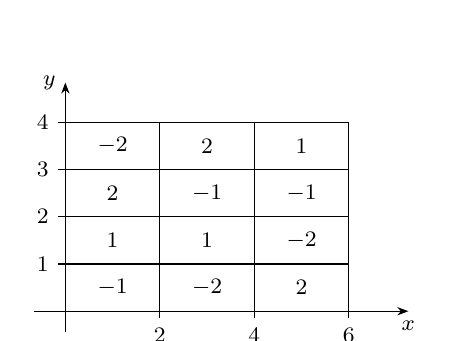
\begin{tikzpicture}[scale=0.6, baseline=(X.base)]
  \def\scale{0.6}
  \node at (0,0) (X) {};

  \drawaxes{0}{0}{6.6}{4.4}

  \foreach \x in {2, 4, 6} {
    \draw (\x, 0) -- (\x, 4);
  }

  \foreach \y in {1, 2, 3, 4} {
    \draw (0, \y) -- (6, \y);
  }

  \foreach \x/\y/\text in {1/0.5/-1, 1/1.5/1, 1/2.5/2, 1/3.5/-2,
                           3/0.5/-2, 3/1.5/1, 3/2.5/-1, 3/3.5/2,
                           5/0.5/2, 5/1.5/-2, 5/2.5/-1, 5/3.5/1} {
    \node at (\x, \y) {$\text$};
  }

  \drawxlabels{2/2, 4/4, 6/6};
  \drawylabels{1/1, 2/2, 3/3, 4/4};
\end{tikzpicture}
\\
(a) & (b)
\end{tabu}
\end{center}
\end{question}

\begin{solution}
\begin{enumerate}
\item
Denote the rectangle $D = [0,4] \x [0,4]$. Because $g$ is a step function, we can evaluate the integral as follows
\[
\iint_D g(x,y) \ud x \ud y =
-2 \cdot 3 + 1 \cdot 9 + 0 \cdot 1 + 3 \cdot 3 = 12\,.
\]
\item
Similarly to the previous exercise, let $D = [0,6] \x [0,4]$. Each smaller rectangle has the same area $2$ and therefore
\begin{align*}
\iint_D g(x,y) \ud x \ud y &=
-2 \cdot \left( -2 + 2 + 1 + 2 -1 -1 + 1 + 1 -2 -1 -2 + 2\right)
= 0\,.
\end{align*}
\end{enumerate}
\end{solution}

\begin{question}
\SetQuestionProperties{source = {Ex. 5; MW, III.17.1}}
Evaluate the iterated integrals
\begin{tasks}(2)
\task
$\displaystyle \int_0^3 \int_0^2 x^3 y \ud x \ud y$.
\task
$\displaystyle \int_0^3 \int_0^2 x^3 y \ud y \ud x$.
\end{tasks}
\end{question}

\begin{solution}
\begin{enumerate}
\item
We have
\begin{align*}
\int_0^3 \int_0^2 x^3 y \ud x \ud y
&= \int_0^3 \frac 14 x^4 y \bigg|_{x=0}^2 \ud y
= 4 \int_0^3 y \ud y = 18\,.
\end{align*}

\item
We have
\begin{align*}
\int_0^3 \int_0^2 x^3 y \ud y \ud x
&= \int_0^3 \frac 12 x^3 y^2 \bigg|_{y=0}^2 \ud x
= \int_0^3 2 x^3 \ud x = \frac{81}{2} \,.
\end{align*}
\end{enumerate}
\end{solution}

\begin{question}
\SetQuestionProperties{source = {Ex. 12, 14--16; MW, III.17.1}}
Evaluate $\displaystyle\iint_{D} f(x,y) \ud x \ud y$ for the following functions and rectangles.
\begin{tasks}(2)
\task
$f(x,y) = xy^3 e^{x^2 y^2}$; $D=[1,3] \x [1,2]$.
\task
$\displaystyle f(x,y) = xy + \frac{x}{y+1}$; $D=[1,4]\x [1,2]$.
\task
$\displaystyle f(x,y) = y^3 \cos^2 x$; $D=[-1,2]\x [0,2]$.

{\itshape Hint:} Use half-angle formulas for $\cos^2 x$.
\task
$\displaystyle f(x,y) = y^5 \sin x\, e^{y^3 \cos x}$; $D=[0,1]\x [-1,0]$.
\end{tasks}
\end{question}

\begin{solution}
\begin{enumerate}
\item
We have
\begin{align*}
\int_1^2 \int_1^3 xy^4 e^{x^2y^2} \ud x \ud y
&= \int_1^2 \frac 12 y e^{x^2y^2} \bigg|_{x=1}^3 \ud y
= \int_1^2 \frac 12 y \left( e^{9y^2} - e^{y^2}\right) \ud y \\
&= \frac{1}{36} e^{9y^2} - \frac{1}{4} e^{y^2} \bigg|_{y=1}^2
= \frac{1}{36} \left(e^{36} - e^9\right) - \frac{1}{4} \left(e^4 - e\right)\,.
\end{align*}
\item We have
\begin{align*}
\int_1^4 \int_1^2 xy + \frac{x}{y+1} \ud y \ud x
&= \int_1^4 x \ud x \int_1^2 y + \frac{1}{y+1} \ud y \\
&= \left(\left. \frac{x^2}2 \right|_{x=1}^4 \right) \left(\left. \frac{y^2}2 + \ln(y+1) \right|_{y=1}^2 \right)
= \frac {45}4 + \frac{15}2 \ln \frac 32\,.
\end{align*}
\item
We have
\begin{align*}
\int_{-1}^2 \int_0^2 y^3 \cos^2 x \ud y \ud x &=
\int_{-1}^2 \frac 14 y^4 \cos^2 x \bigg|_{y=0}^2 \ud x
= \int_{-1}^2 4 \cos^2 x \ud x 
= \int_{-1}^2 2 + 2\cos 2x \ud x \\
&= 2x + \sin 2x \bigg|_{x={-1}}^2 = 6 + \sin 2 + \sin 4\,.
\end{align*}
\item
We choose the following order of integration
\begin{align*}
\int_{-1}^0 \int_0^1 y^5 \sin x\, e^{y^3 \cos x} \ud x \ud y
&= \int_{-1}^0 -y^2 e^{y^3 \cos x} \bigg|_{x=0}^1 \ud y
= \int_{-1}^0 -y^2 e^{y^3 \cos 1} + y^2 e^{y^3}\ud y \\
&= \left.\frac{-1}{3\cos 1} e^{y^3 \cos 1} + \frac 13 e^{y^3} \right|_{y=-1}^0 \\
&= \frac 13 - \frac 1{3e} + \frac{1}{3\cos 1}\left(e^{-\cos 1} - 1\right)\,.
\end{align*}
\end{enumerate}
\end{solution}

\begin{question}
\SetQuestionProperties{source = {Ex. 19; MW, III.17.1}}
Find the volume under the graph of
\[
f(x,y) = x^3 + y^2 + 2\,,
\]
between the planes
\[
x=-1, x=1, y=1 \text{ and } y=3\,.
\]
\end{question}

\begin{solution}
The volume is given by the integral
\begin{align*}
\iint_{[-1,1]\times [1,3]} x^3 + y^2 + 2 \ud x \ud y
&= \int_{-1}^1 \int_1^3 x^3 + y^2 + 2 \ud y \ud x \\
&= \int_{-1}^1 x^3y + \frac 13 y^3 + 2y \bigg|_{y=1}^3 \ud x
= \int_{-1}^1 2x^3 + \frac{38}3 \ud x \\
&= \frac 12 x^4 + \frac{38}3x \bigg|_{x=-1}^1 = \frac{76}{3}\,.
\end{align*}
\end{solution}

\begin{question}
\SetQuestionProperties{source = {Ex. 21; MW, III.17.1}}
The density at each point of a $1$ centimeter square (i.e., each side has length $1$ centimeter) microchip is $4+r^2$ grams per square centimeter, where $r$ is the distance in centimeters from the point to the center of the chip. What is the mass of the chip?
\end{question}

\begin{solution}
We model the chip as the rectangle $D = \left[-\frac 12, \frac 12\right] \x \left[-\frac 12, \frac 12\right]$. Then the center is the point $(0,0)$ and the squared distance of a point $(x,y)$ to the center is $r^2 = x^2 + y^2$. Thus the mass $m$ can be computed as
\begin{align*}
m &= \int_{-1/2}^{1/2} \int_{-1/2}^{1/2} 4 + x^2 + y^2 \ud x \ud y
= \int_{-1/2}^{1/2} 4x + \frac 13 x^3 + xy^2 \bigg|_{x={-1/2}^{1/2}} \ud y
= \int_{-1/2}^{1/2} 4 + \frac 1{12} + y^2 \ud y \\
&= 4y + \frac 1{12}y + \frac 13 y^3 \bigg|_{y=-1/2}^{1/2}
= 4 + \frac 1{12} + \frac{1}{12} = \frac{25}{6}\,.
\end{align*}
\end{solution}

\begin{question}
\SetQuestionProperties{difficulty={*}}
Using the fact that for $x,y > 0$,
\[
\frac{\p^2}{\p x \p y} \arctan \frac xy = \frac{x^2-y^2}{\left(x^2 + y^2 \right)^2}\,,
\]
show that
\begin{align*}
\int_0^1 \left( \int_0^1 \frac{x^2-y^2}{\left(x^2 + y^2 \right)^2} \ud y \right) \ud x
&= \frac \pi 4 &
\int_0^1 \left( \int_0^1 \frac{x^2-y^2}{\left(x^2 + y^2 \right)^2} \ud x \right) \ud y
&= -\frac \pi 4\,.
\end{align*}

\begin{note*}
This problem shows that the order of integration sometimes does matter. The problem here is that the function $\frac{x^2-y^2}{\left(x^2 + y^2 \right)^2}$ is not integrable over the rectangle $R = [0,1] \x [0,1]$, which means that we cannot apply the theorem, that reduces the double integral to an iterated integral; the double integral $\iint_R \frac{x^2-y^2}{\left(x^2 + y^2 \right)^2} \ud x \ud y$ does not exist. This example was found already by Cauchy in 1814\footfullcite[p.178]{Elstrodt2011}.
\end{note*}
\end{question}

%%% Local Variables:
%%% TeX-master: "problems"
%%% End:

\ifthenelse{\boolean{sectionnewpage}}{\newpage}{}

\section{The Double Integral over General Regions}
\begin{question}
Find an example for each of the following domains.
\begin{tasks}(2)
\task
A domain of type 1 and type 2.
\task
A domain of neither type 1 nor type 2.
\task
A domain of type 1, but not of type 2.
\task
A domain of type 2, but not of type 1.
\end{tasks}
\end{question}

\begin{solution}
Examples of domains can be found below.
\begin{center}
\begin{figuretable}{4}
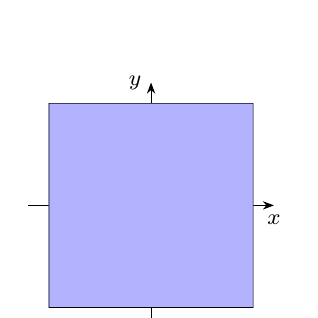
\begin{tikzpicture}[scale=1.3, baseline=(X.base)]
  \def\scale{1.3}
  \node at (0,-1) (X) {};

  \drawaxes{-1}{-1}{1}{1}
  \clip (-1,-1) rectangle (1,1);

  \draw[integration domain] (1,1) |- (-1,-1) |- cycle;
\end{tikzpicture}
&
\begin{tikzpicture}[scale=1.3, baseline=(X.base)]
  \def\scale{1.3}
  \node at (0,-1) (X) {};

  \drawaxes{-1}{-1}{1}{1}
  \clip (-1,-1) rectangle (1,1);

  \draw[integration domain]
    plot[parametric, domain=-1:1, samples=100] function {t, 0.5*t**2+0.5}
    -- plot[parametric, domain=1:-1, samples=100] function {0.5*t**2+0.5, t}
    -- plot[parametric, domain=1:-1, samples=100] function {t, -0.5*t**2-0.5}
    -- plot[parametric, domain=-1:1, samples=100] function {-0.5*t**2-0.5, t};
\end{tikzpicture}
&
\begin{tikzpicture}[scale=1.3, baseline=(X.base)]
  \def\scale{1.3}
  \node at (0,-1) (X) {};

  \drawaxes{-1}{-1}{1}{1}
  \clip (-1,-1) rectangle (1,1);

  \draw[integration domain]
    plot[parametric, domain=-1:1, samples=100] function {t, 0.5*t**2+0.5}
    -- (1,-1)
    -- plot[parametric, domain=1:-1, samples=100] function {t, -0.5*t**2-0.5}
    -- (-1,1);
\end{tikzpicture}
&
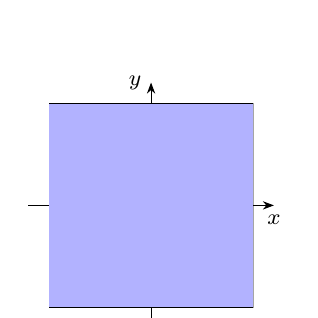
\begin{tikzpicture}[scale=1.3, baseline=(X.base)]
  \def\scale{1.3}
  \node at (0,-1) (X) {};

  \drawaxes{-1}{-1}{1}{1}
  \clip (-1,-1) rectangle (1,1);

  \draw[integration domain]
    (-1,1) -- (1,1)
    -- plot[parametric, domain=1:-1, samples=100] function {0.5*t**2+0.5, t}
    -- (1,-1) -- (-1,-1)
    -- plot[parametric, domain=-1:1, samples=100] function {-0.5*t**2-0.5, t};
\end{tikzpicture}
\\
(a) & (b) & (c) & (d)
\end{figuretable}
\end{center}
\end{solution}

\begin{question}
\SetQuestionProperties{source = {Ex. 1--2; MW, III.17.2}}
Sketch each of the following domains and determine whether it is of type 1, type 2, both or neither.
\begin{tasks}(2)
\task
$(x,y)$ such that $0 \leq y \leq 3x$, $0 \leq x \leq 1$.
\task
$(x,y)$ such that $2y^2-1 \leq x \leq y^2$, $|y| \leq 1$.
\task
$(x,y)$ such that $y^2 \leq x \leq y$, $0 \leq y \leq 1$.
\task
$(x,y)$ such that $1 - x^2 \leq 2y$, $x^2+y^2 \leq 1$.
\task
$(x,y)$ such that $x^2 + y^2 \leq 1$.
\task
$(x,y)$ such that $\displaystyle \frac 12 \leq x^2 + y^2 \leq 1$.
\end{tasks}
\end{question}

\begin{solution}
The domains can be seen in the figures below.
% \begin{center}
% \begin{figuretable}{3}
% \begin{tikzpicture}[scale=1.25, baseline=0]
%   \def\scale{1.25}

%   \drawxlabels{1/1}
%   \drawylabels{3/3}
%   \drawaxes{0}{0}{3}{3}

%   \draw[dashed] (0,3) -- (1,3);

%   \draw[integration domain] (0,0) -- (1,0) -- (1,3) -- (0,0);
%   \node at (0.66,1) {$D$};
% \end{tikzpicture}
% &
% \begin{tikzpicture}[scale=1.25, baseline=(X.base)]
%   \def\scale{1.25}
%   \node at (0,-1.5) (X) {};

%   \drawaxes{-1.5}{-1.5}{1.5}{1.5}

%   \node[above left] at (-.5,.5) {$x=2y^2-1$};
%   \node[below right] at (.5,.7) {$x=y^2$};

%   \clip (-1.5,-1.5) rectangle (1.5,1.5);

%   \draw[dashed] (0,1) -- (1,1)
%                 (0,-1) -- (1,-1);

%   \fill[integration domain]
%     plot[parametric, domain=-1:1, samples=100] function {2*t**2-1, -t}
%     --plot[parametric, domain=-1:1, samples=100] function {t**2, t};

%   \draw plot[parametric, domain=-1.5:1.5, samples=100] function {2*t**2-1, t};
%   \draw plot[parametric, domain=-1.5:1.5, samples=100] function {t**2, t};

%   \node at (-0.5,0) {$D$};

%   \drawylabels[nofill]{-1/-1, 1/1}
% \end{tikzpicture}
% &
% \begin{tikzpicture}[scale=2.5, baseline=(X.base)]
%   \def\scale{2.5}
%   \node at (0,-0.25) (X) {};

%   \drawaxes{-0.25}{-0.25}{1.25}{1.25}
%   \drawxlabels{1/1}
%   \drawylabels{1/1}

%   \draw[dashed] (1,0) -- (1,1) -- (0,1);

%   \clip (-0.25,-0.25) rectangle (1.25,1.25);

%   \fill[integration domain] (0,0) -- (1,1) 
%     --plot[domain=1:0, samples=100] function {sqrt(x)};
%   \draw (-0.25,-0.25) -- (1.25,1.25);
%   \draw plot[parametric, domain=-0.25:1.25, samples=100] function {t**2, t};

%   \node[below right] at (0.25,0.25) {$x=y$};
%   \node[above left] at (0.5,0.707) {$x=y^2$};
%   \node at (0.375,0.5) {$D$};
% \end{tikzpicture}
% \\
% (a) & (b) & (c)
% \end{figuretable}
% \end{center}

\begin{center}
\begin{figuretable}{3}
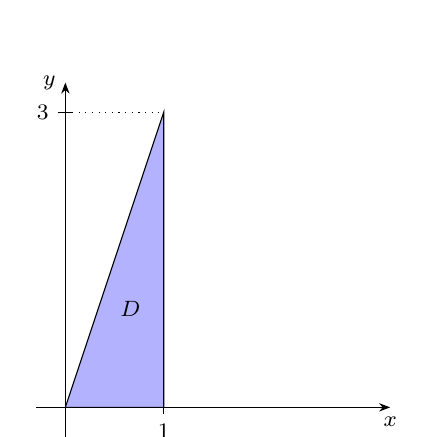
\begin{tikzpicture}[scale=1.25, baseline=0]
  \def\scale{1.25}

  \drawxlabels{1/1}
  \drawylabels{3/3}
  \drawaxes{0}{0}{3}{3}

  \draw[dotted] (0,3) -- (1,3);

  \draw[integration domain] (0,0) -- (1,0) -- (1,3) -- (0,0);
  \node at (0.66,1) {$D$};
\end{tikzpicture}
&
\begin{tikzpicture}[scale=1.25, baseline=(X.base)]
  \def\scale{1.25}
  \node at (0,-1.5) (X) {};

  \drawaxes{-1.5}{-1.5}{1.5}{1.5}

  \node[above left] at (-.5,.5) {$x=2y^2-1$};
  \node[below right] at (.5,.7) {$x=y^2$};

  \clip (-1.5,-1.5) rectangle (1.5,1.5);

  \draw[dotted] (0,1) -- (1,1)
                (0,-1) -- (1,-1);

  \draw[integration domain]
    plot[parametric, domain=-1:1, samples=100] function {2*t**2-1, -t}
    --plot[parametric, domain=-1:1, samples=100] function {t**2, t};

  \draw[dashed]
     plot[parametric, domain=1:1.5, samples=100] function {2*t**2-1, t}
     plot[parametric, domain=-1.5:-1, samples=100] function {2*t**2-1, t};
  \draw[dashed]
    plot[parametric, domain=1:1.5, samples=100] function {t**2, t}
    plot[parametric, domain=-1.5:-1, samples=100] function {t**2, t};

  \node at (-0.5,0) {$D$};

  \drawylabels[nofill]{-1/-1, 1/1}
\end{tikzpicture}
&
\begin{tikzpicture}[scale=2.5, baseline=(X.base)]
  \def\scale{2.5}
  \node at (0,-0.25) (X) {};

  \drawaxes{-0.25}{-0.25}{1.25}{1.25}
  \drawxlabels{1/1}
  \drawylabels{1/1}

  \draw[dotted] (1,0) -- (1,1) -- (0,1);

  \clip (-0.25,-0.25) rectangle (1.25,1.25);

  \draw[integration domain] (0,0) -- (1,1) 
    --plot[domain=1:0, samples=100] function {sqrt(x)};
  \draw[dashed] (-0.25,-0.25) -- (0,0)
                (1,1) -- (1.25,1.25);
  \draw[dashed]
    plot[parametric, domain=-0.25:0, samples=100] function {t**2, t}
    plot[parametric, domain=1:1.25, samples=100] function {t**2, t};

  \node[below right] at (0.5,0.5) {$x=y$};
  \node[above left] at (0.5,0.707) {$x=y^2$};
  \node at (0.375,0.5) {$D$};
\end{tikzpicture}
\\
(a) & (b) & (c)
\end{figuretable}
\end{center}

\begin{enumerate}
\item
The domain is a triangle with vertices $(0,0)$, $(1,0)$ and $(1,3)$. It is a domain of both types.
\item
This domain can be written as
\[
D = \left\{ (x,y) \,:\, -1 \leq y \leq 1,\, 2y^2 - 1 \leq x \leq y^2 \right\}\,.
\]
It is a type 2 domain, but not a type 1 domain.
\item
This domain can be written as
\begin{align*}
D &= \left\{ (x,y) \,:\, 0 \leq y \leq 1\,,\; y^2 \leq x \leq y \right\}
= \left\{ (x,y) \,:\, 0 \leq x \leq 1\,,\; x \leq y \leq \sqrt{x} \right\}\,,
\end{align*}
and hence it is a domain of both types.
\item
The domain can be written as
\[
D = \left\{ (x,y) \,:\, -1 \leq x \leq 1,\, \frac 12\left(1-x^2\right) \leq y \leq \sqrt{1-x^2} \right\}\,.
\]
It is a type 1 domain, but not a type 2 domain.
\item
The domain can be written as
\begin{align*}
D &= \left\{ (x,y) \,:\, -1 \leq y \leq 1\,,\; -\sqrt{1-y^4} \leq x \leq \sqrt{1-y^4} \right\} \\
&= \left\{ (x,y) \,:\, -1 \leq x \leq 1\,,\; -\sqrt{1-x^4} \leq y \leq \sqrt{1-x^4} \right\}\,,
\end{align*}
and it is a domain of both types.
\item
This domain is neither of type 1 nor of type 2.
\end{enumerate}

\begin{center}
\begin{figuretable}{3}
\begin{tikzpicture}[scale=1.875, baseline=(X.base)]
  \def\scale{1.875}
  \node at (0,-1) (X) {};

  \drawaxes{-1}{-1}{1}{1}

  \draw[integration domain] 
    plot[domain=-1:1, samples=100] function {0.5-0.5*x**2}
    --(1,0) arc[start angle=0, end angle=180, radius=1];

  \draw[dashed]
    (-1,0) arc[radius=1, start angle=180, end angle=360];
%  \draw plot[domain=-1:1, samples=100] function {0.5-0.5*x**2};

  \node at (0,0.75) {$D$};

  \drawxlabels[fill]{-1/-1, 1/1}
  \drawylabels[nofill]{1/1}
  \drawylabels[fill]{-1/-1}
\end{tikzpicture}
&
\begin{tikzpicture}[scale=1.875, baseline=(X.base)]
  \def\scale{1.875}
  \node at (0,-1) (X) {};

  \draw[integration domain, samples=100, smooth]
    plot[parametric, domain=0:3.1416/2] 
      function {cos(t), sin(t)}
    --plot[parametric, domain=3.1416/2:3.1416] 
      function {-(abs(cos(t))), sin(t)}
    --plot[parametric, domain=3.1416:3.1416*1.5] 
      function {-abs(cos(t)), -abs(sin(t))}
    --plot[parametric, domain=3.1416*1.5:3.1416*2] 
      function {cos(t), -abs(sin(t))}
    --(1,0) ;

  % Coordinate axes
  \drawaxes{-1}{-1}{1}{1}
  \drawxlabels[nofill]{-1/-1, 1/1}
  \drawylabels[nofill]{-1/-1, 1/1}

  % Label
  \node at (0.4,0.4) {$D$};
\end{tikzpicture}
&
\begin{tikzpicture}[scale=1.875, baseline=(X.base)]
  \def\scale{1.875}
  \node at (-1,-1) (X) {};

  \def\r{0.707106} % sqrt(2)/2

  % Draw both curves at the same time and use even odd rule to plot inside
  \draw[integration domain, samples=100, smooth, even odd rule]
    plot[parametric, domain=0:3.1416/2] 
      function {cos(t), sin(t)}
    --plot[parametric, domain=3.1416/2:3.1416] 
      function {-(abs(cos(t))), sin(t)}
    --plot[parametric, domain=3.1416:3.1416*1.5] 
      function {-abs(cos(t)), -abs(sin(t))}
    --plot[parametric, domain=3.1416*1.5:3.1416*2] 
      function {cos(t), -abs(sin(t))}
    --(1,0)
    plot[parametric, domain=0:3.1416/2] 
      function {\r*cos(t), \r*sin(t)}
    --plot[parametric, domain=3.1416/2:3.1416] 
      function {-\r*(abs(cos(t))), \r*sin(t)}
    --plot[parametric, domain=3.1416:3.1416*1.5] 
      function {-\r*abs(cos(t)), -\r*abs(sin(t))}
    --plot[parametric, domain=3.1416*1.5:3.1416*2] 
      function {\r*cos(t), -\r*abs(sin(t))}
    --(\r,0) ;

  % Coordinate axes
  \drawaxes{-1}{-1}{1}{1}
  \drawxlabels[nofill]{-1/-1, \r/\textstyle{\frac{\sqrt{2}}{2}}, 1/1}
  \drawylabels[nofill]{-1/-1, 1/1}

  % Label
  \node at (0.4,0.75) {$D$};
\end{tikzpicture}
\\
(d) & (e) & (f)
\end{figuretable}
\end{center}
\end{solution}

\begin{question}
\SetQuestionProperties{source = {Ex. 5; Guichard, 15.1}}
Evaluate the following iterated integrals.
\begin{tasks}(2)
\task
$\int_0^1 \int_0^y xy \ud x \ud y$
\task
$\int_1^4 \int_1^{\sqrt{x}} y^2 \ud y \ud x$.
\task
$\int_1^2 \int_{y^2/2}^{\sqrt y} 1 \ud x \ud y$
\task
$\int_1^2 \int_1^x \frac{x^2}{y^2} \ud y \ud x$
\task
$\int_0^1 \int_0^x \frac{y}{e^x} \ud y \ud x$
\task
$\int_0^{\sqrt{\pi}/2} \int_0^{x^2} x \cos y \ud y \ud x$
\end{tasks}
\end{question}

\begin{solution}
\begin{enumerate}
\item
\begin{alignenum}
\int_0^1 \int_0^y xy \ud x \ud y
= \int_0^1 \frac 12 x^2 y \bigg|_{x=0}^y \ud y
= \frac 12 \int_0^1 y^3 \ud y
= \frac 18\,.
\end{alignenum}
\item
\begin{alignenum}  
\int_1^4 \int_1^{\sqrt{x}} y^2 \ud y \ud x
&= \int_1^4 \frac 13 y^3 \bigg|_{y=1}^{\sqrt{x}} \ud x
= \int_1^4 \frac 13 x^{3/2} - \frac 13 \ud x 
= \frac 2{15} x^{5/2} - \frac 13 x \bigg|_{x=1}^4
%= \frac{64}{15} - \frac 4 3 - \frac 2{15} + \frac 13
= \frac{47}{15}\,.
\end{alignenum}
\item
\begin{alignenum}
\int_1^2 \int_{y^2/2}^{\sqrt y} 1 \ud x \ud y
= \int_1^2 \sqrt{y} - \frac 12 y^2 \ud y
= \frac 23 y^{3/2} - \frac 16 y^3 \bigg|_{y=1}^2
= \frac{4}{3}\sqrt{2} - \frac{11}{6}\,.
\end{alignenum}
\item
\begin{alignenum}
\int_1^2 \int_1^x \frac{x^2}{y^2} \ud y \ud x
= \int_1^2 -\frac{x^2}{y} \bigg|_{y=1}^x \ud x
= \int_1^2 -x + x^2 \ud x 
= -\frac 12 x^2 + \frac 13 x^3\bigg|_{x=1}^2
= \frac{5}{6}\,.
\end{alignenum}
\item
\begin{alignenum}
\int_0^1 \int_0^x \frac{y}{e^x} \ud y \ud x
&= \int_0^1 \frac 12 \frac{y^2}{e^x} \bigg|_{y=0}^x \ud x
= \frac 12 \int_0^1 x^2 e^{-x} \ud x
= -\frac 12 x^2 e^{-x}\bigg|_{x=0}^1 + \int_0^1 x e^{-x} \ud x \\
&= -\frac 12 e^{-1} - x e^{-x} \bigg|_{x=0}^1 + \int_0^1 e^{-x} \ud x
= -\frac 32 e^{-x} - e^{-x}|_{x=0}^1 = 1-\frac 52 e^{-x}\,.
\end{alignenum}
\item
\begin{alignenum}
\int_0^{\sqrt{\pi}/2} \int_0^{x^2} x \cos y \ud y \ud x
%= \int_0^{\sqrt{\pi}/2} x \sin y \bigg|_{y=0}^{x^2} \ud x
= \int_0^{\sqrt{\pi}/2} x \sin\left(x^2\right) \ud x
= -\frac 12 \cos \left(x^2\right) \bigg|_{x=0}^{\sqrt{\pi}/2} = \frac 12 - \frac{\sqrt 2}4\,.
\end{alignenum}
\end{enumerate}
\end{solution}

\begin{question}
\SetQuestionProperties{source = {Ex. 9--11; Thomas 12th, 15.2}}
Write an iterated integral $\iint_D f(x,y) \ud x \ud y$ over the described region, both as a type 1 domain and as a type 2 domain.
\begin{center}
\begin{figuretable}{3}
\begin{tikzpicture}[scale=1.875, baseline=(X.base)]
  \def\scale{1.875}
  \node at (0,-0.5) (X) {};

  \drawaxes{-0.5}{-0.5}{1.5}{1.5}
  \clip (-.5,-.5) rectangle (1.5,1.5);

  \draw plot[parametric, domain=-0.5:1.5, samples=100] function {t, t**3};
  \draw (-.5,1) -- (1.5,1);

  \draw[integration domain]
    plot[parametric, domain=0:1, samples=100] function {t, t**3}
    -- (0,1) -- (0,0);

  \node[below right] at (1,1) {$y=8$};
  \node[left] at (1.1, {1.1^3}) {$y=x^3$};

  \node at (0.4,0.6) {$D$};
\end{tikzpicture}
&
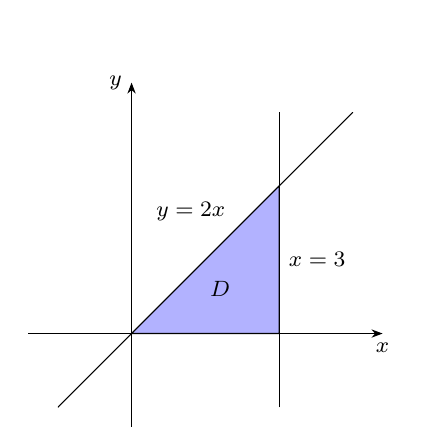
\begin{tikzpicture}[scale=1.875, baseline=(X.base)]
  \def\scale{1.875}
  \node at (0,-0.5) (X) {};

  \drawaxes{-0.5}{-0.5}{1.5}{1.5}
  \clip (-.5,-.5) rectangle (1.5,1.5);

  \draw (-.5,-.5) -- (1.5,1.5);
  \draw (1,-.5) -- (1,1.5);

  \draw[integration domain]
    (0,0) -- (1,0) -- (1,1) -- cycle;

  \node[right] at (1,.5) {$x=3$};
  \node[above left] at (.7,.7) {$y=2x$};

  \node at (0.6,0.3) {$D$};
\end{tikzpicture}
&
\begin{tikzpicture}[scale=1.875, baseline=(X.base)]
  \def\scale{1.875}
  \node at (0,-0.5) (X) {};

  \drawaxes{-0.5}{-0.5}{1.5}{1.5}
  \clip (-.5,-.5) rectangle (1.5,1.5);

  \draw plot[parametric, domain=-0.5:1.5, samples=100] function {t, t**2};
  \draw (-.5,-.5) -- (1.5,1.5);

  \draw[integration domain]
    plot[parametric, domain=0:1, samples=100] function {t, t**2}
    -- (0,0);

  \node[left] at (.8,.8) {$y=3x$};
  \node[right] at (0.7, 0.49) {$y=x^2$};

  \node at (0.5,0.375) {$D$};
\end{tikzpicture}
\\
(a) & (b) & (c)
\end{figuretable}
\end{center}
\end{question}

\begin{solution}
\begin{enumerate}
\item
The functions $y=x^3$ and $y=8$ intersect in the point $(2,8)$ and the inverse of $y=x^3$ is $x=\sqrt[3]{y}$. Thus
\[
\iint_D f(x,y) \ud x \ud y
= \int_0^2 \int_{x^3}^8 f(x,y) \ud y \ud x
= \int_0^8 \int_0^{\sqrt[3]{y}} f(x,y) \ud x \ud y\,.
\]
\item
The lines $y=2x$ and $x=3$ intersect in the point $(3,6)$ and the iverse of $y=2x$ is $x=\frac y2$. Thus
\[
\iint_D f(x,y) \ud x \ud y
= \int_0^3 \int_0^{2x} f(x,y) \ud y \ud x
= \int_0^6 \int_{y/2}^3 f(x,y) \ud x \ud y\,.
\]
\item
The functions $y=3x$ and $y=x^2$ intersect in the two points $(0,0)$ and $(3,9)$. The inverse of $y=3x$ is $x=\frac y3$ and the inverse of $y=x^2$ is $x=\sqrt y$. Thus
\[
\iint_D f(x,y) \ud x \ud y
= \int_0^3 \int_{x^2}^{3x} f(x,y) \ud y \ud x
= \int_0^9 \int_{y/3}^{\sqrt y} f(x,y) \ud x \ud y\,.
\]
\end{enumerate}
\end{solution}

\begin{question}
\SetQuestionProperties{source = {Ex. 21, 22; MW, III.17.2 and Ex. 13, 16, 17; Hartman, 13.2}}
Evaluate the following integrals
\begin{tasks}(1)
\task
$\iint_D 3-y \ud x \ud y$; $D$ is the domain between the parabolas $y^2=2x$ and $x^2=2y$.
\task
$\iint_D x^2-y^2 \ud x \ud y$; $D$ is the rectangle with vertices $(-1,-1)$, $(1,-1)$, $(1,1)$, $(-1,1)$.
\task
$\iint_D x^3y - x \ud x \ud y$; $D$ is the half of the circle $x^2 + y^2 \leq 9$ in the first and second quadrants.
\task
$\iint_D x-y \ud x \ud y$; $D$ is the triangle with vertices $(0,0)$, $(1,0)$ and $(2,2)$.
\task
$\iint_D y \cos x \ud x \ud y$; $D$ is the triangle defined by $0 \leq x \leq \pi$ and $0 \leq y \leq x$.
\task
\difficulty{*}
$\iint_D e^y \ud x \ud y$; $D$ is the domain between $y=\ln x$ and $y = \frac{1}{e-1}(x-1)$.
\end{tasks}
\end{question}

\begin{solution}
\begin{center}
\begin{figuretable}{3}
\begin{tikzpicture}[scale=1.25, baseline=(X.base)]
  \def\scale{1.25}
  \node at (0,-.5) (X) {};

  \drawaxes{-.5}{-.5}{2.5}{2.5}
  \clip (-.5,-.5) rectangle (2.5,2.5);

  \draw[dotted] (0,2) -- (2,2) -- (2,0);

  \draw[integration domain] 
    plot[parametric, domain=0:2, samples=100] function {t, sqrt(2*t)}
    -- plot[parametric, domain=2:0, samples=100] function {t, t**2/2};

  \draw[dashed]
    plot[parametric, domain=-0.5:0, samples=100] function {t, t**2/2}
    plot[parametric, domain=2:2.5, samples=100] function {t, t**2/2};
  \draw[dashed]
    plot[parametric, domain=-0.5:0, samples=100] function {t**2/2, t}
    plot[parametric, domain=2:2.5, samples=100] function {t**2/2, t};

  \node[left] at (1.2,{sqrt{2*1.2}}) {$x=y^2/2$};
  \node[right] at (.75,{.7^2/2}) {$x=\sqrt{2y}$};
  \node at (1,1) {$D$};

  \drawxlabels[fill]{2/2}
  \drawylabels[fill]{2/2}
\end{tikzpicture}
&
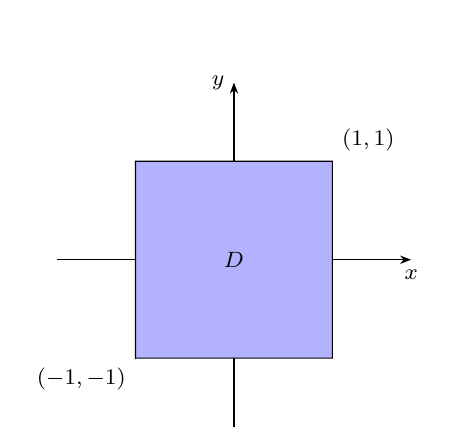
\begin{tikzpicture}[scale=1.25, baseline=(X.base)]
  \def\scale{1.25}
  \node at (0,-1.5) (X) {};

  \drawaxes{-1.5}{-1.5}{1.5}{1.5}

  \draw[integration domain] (-1,-1) -| (1,1) -| cycle;

  \node[above right] at (1,1) {$(1,1)$};
  \node[below left] at (-1,-1) {$(-1,-1)$};
  
  \node at (0,0) {$D$};
\end{tikzpicture}
&
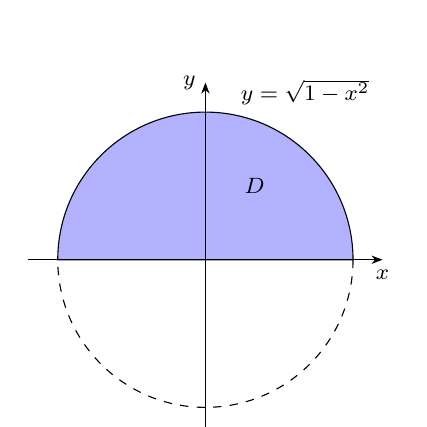
\begin{tikzpicture}[scale=0.625, baseline=(X.base)]
  \def\scale{0.625}
  \node at (-3,-3) (X) {};

  \draw[integration domain]
    (3,0) arc[radius=3, start angle=0, end angle=180] -- cycle;

  \draw[dashed]
    (3,0) arc[radius=3, start angle=0, end angle=-180];

  % Coordinate axes
  \drawaxes{-3}{-3}{3}{3}
  % \drawxlabels[fill]{-3/-3,3/3}
  % \drawylabels[nofill]{-3/-3,3/3}

  \node[above right] at (80:3) {$y=\sqrt{1-x^2}$};

  % Label
  \node at (1,1.5) {$D$};
\end{tikzpicture}
\\
(a) & (b) & (c)
\end{figuretable}
\end{center}

\begin{enumerate}
\item
The domain can be written as a type 2 domain with lower limit $x=\frac{y^2}2$ and upper limit $x = \sqrt{2y}$. Thus
\begin{align*}
\iint_D 3-y \ud x \ud y
&= \int_0^2 \int_{y^2/2}^{\sqrt{2y}} 3-y \ud x \ud y
= \int_0^2 (3-y)\left(\sqrt{2y} - \frac{y^2}{2} \right) \ud y \\
&= \int_0^2 3\sqrt 2 y^{1/2} - \sqrt 2 y^{3/2} - \frac 32 y^2 + \frac 12 y^3 \ud y \\
&= 2 \sqrt 2 y^{3/2} - \frac 25 \sqrt 2 y^{5/2} - \frac 12 y^3 + \frac 18 y^4 \bigg|_{y=0}^2
= \frac {14}5\,.
\end{align*}
\item
This is a simple iterated integral with fixed limits.
\[
\int_{-1}^1 \int_{-1}^1 x^2 - y^2 \ud x \ud y
= \int_{-1}^1 \frac 13 x^3 - xy^2 \bigg|_{x=-1}^1 \ud y
= \int_{-1}^1 \frac 23 - 2y^2 \ud y = 0\,.
\]
\item
This domain is of type 1 with lower limit $y=0$ and upper limit $y=\sqrt{3-x^2}$. Thus
\begin{align*}
\int_{-3}^3 \int_0^{\sqrt{3-x^2}} x^3 y - x \ud y \ud x
&= \int_{-3}^3 \frac 12 x^3 y^2 - xy \bigg|_{y=0}^{\sqrt{3-x^2}} \ud x
= \int_{-3}^3 \frac 12 x^3 \left(3-x^2 \right) - x \sqrt{3-x^2} \ud x \\
&= \frac 38 x^4 - \frac 1{12}x^6 + \frac 13 \left(3-x^2\right)^{3/2} \bigg|_{x=-3}^3
=0 \,.
\end{align*}
\item
The triangle is a type 2 domain and can be parametrised by
\[
D = \left\{ (x,y) \,:\, 0 \leq y \leq 2\,,\; y \leq x \leq \frac y2+1 \right\}
\]
We then have to calculate the integral
\begin{align*} 
\iint_D x-y \ud x \ud y
&= \int_0^2 \int_{y}^{y/2-2} x-y \ud x \ud y 
= \int_0^2 \frac 12 x^2 - xy \bigg|_{x=y}^{y/2-2} \ud y \\
&= \int_0^1 \frac 12 \left(\frac y2-2\right)^2 - \frac {y^2}{2} - y\left(\frac y2-2\right) + y^2 \ud y \\
&= \int_0^2 \frac{y^2}8 + y + 2 \ud y
= \frac 13 + 2 + 4 = \frac {19}3 \,.
\end{align*}
\item
This integral is best written as an integral over a type 2 domain.
\begin{align*}
\iint_D y \cos x \ud x \ud y
&= \int_0^\pi \int_y^\pi y \cos x \ud x \ud y
= \int_0^\pi y \sin x \bigg|_{x=y}^\pi \ud y
= - \int_0^\pi y \sin y \ud y \\
&= y \cos y \bigg|_{y=0}^\pi + \int_0^\pi \cos y \ud y
= -\pi\,.
\end{align*}
\item
The challenge here is to find the limits of integration. These are given by solutions of
\[
\ln x = \frac {1}{e-1} \left(x-1\right)\,.
\]
The two solutions are given by $x=1$ and $x=e$. The domain is of type 1 and therefore
\begin{align*}
\iint_D e^y \ud x \ud y
&= \int_1^e \int_{\ln x}^{(x-1)/(e-1)} e^y \ud y \ud x
= \int_1^e e^{(x-1)/(e-1)} - x \ud x \\
&= (e-1) e^{(x-1)/(e-1)} - \frac 12 x^2 \bigg|_{x=1}^e
= \frac 32 + \frac 12 e^2\,.
\end{align*}
\end{enumerate}
\begin{center}
\begin{figuretable}{3}
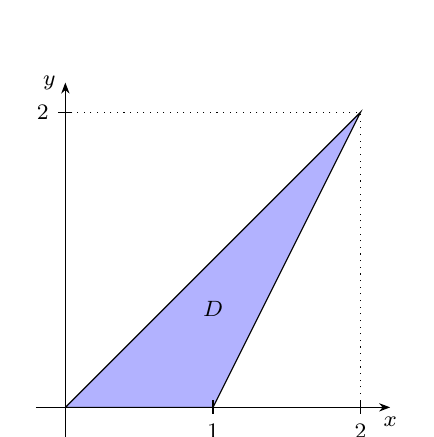
\begin{tikzpicture}[scale=1.875, baseline=(X.base)]
  \def\scale{1.875}
  \node at (0,0) (X) {};

  \drawaxes{0}{0}{2}{2}

  \draw[dotted] (2,0) -- (2,2) -- (0,2);

  \draw[integration domain]
    (0,0) -- (1,0) -- (2,2) -- cycle;

  \node at (1,0.666) {$D$};

  \drawxlabels[fill]{1/1, 2/2}
  \drawylabels[fill]{2/2}
\end{tikzpicture}
&
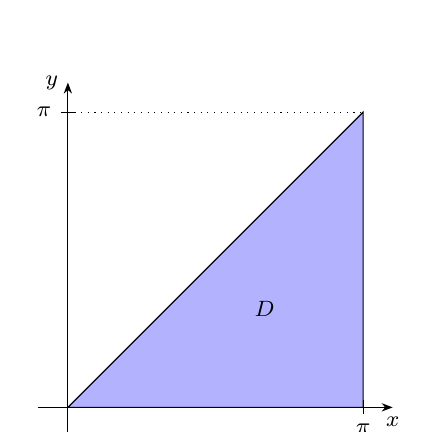
\begin{tikzpicture}[scale=3.75, baseline=(X.base)]
  \def\scale{3.75}
  \node at (0,0) (X) {};

  \drawaxes{0}{0}{1}{1}

  \draw[dotted] (0,1) -- (1,1);

  \draw[integration domain] 
    (0,0) -- (1,0) -- (1,1) -- cycle;
  
  \node at (0.666,0.333) {$D$};
  
  \drawxlabels{1/\pi};
  \drawylabels{1/\pi};
\end{tikzpicture}
&
\begin{tikzpicture}[scale=1.25, baseline=(X.base)]
  \def\scale{1.25}
  \node at (0,-1.5) (X) {};

  \drawaxes{0}{-1.5}{3}{1.5}

  \drawxlabels{1/1, 2.787/e}
  \drawylabels{1/1}

  \clip (0,-1.5) rectangle (3,1.5);

  \draw[dotted] (2.787,0) -- (2.787,1) -- (0,1);

  \draw[dashed]
    plot[parametric, domain=0.01:1, samples=100] function {t, log(t)}
    plot[parametric, domain=2.787:3, samples=100] function {t, log(t)};

  \draw[dashed] (0,{-1/(2.787-1)}) -- (1,0)
                (2.787,1) -- (3,{2/(2.787-1)});

  \draw[integration domain]
    plot[parametric, domain=1:2.787, samples=100] function {t, log(t)} -- cycle;

  \node at (1.9, 0.55) {$D$};
\end{tikzpicture}
\\
(d) & (e) & (f)
\end{figuretable}
\end{center}
\end{solution}

\begin{question}
Interpret the following iterated integrals as double integrals over a domain $D$. Sketch $D$ and change the order of integration.
\begin{tasks}(2)
\task
$\int_0^3 \int_0^{\sqrt{3}} f(x,y) \ud y \ud x$
\task
$\int_1^3 \int_0^{\ln x} f(x,y) \ud y \ud x$
\task
$\int_0^1 \int_{\arctan y}^{\pi/4} f(x,y) \ud x \ud y$
\task
$\int_{-\sqrt 2}^{\sqrt 2} \int_{y^2-1}^1 f(x,y) \ud x \ud y$
\end{tasks}
\end{question}

\begin{solution}
The domains can be seen below.
\begin{center}
\begin{figuretable}{4}
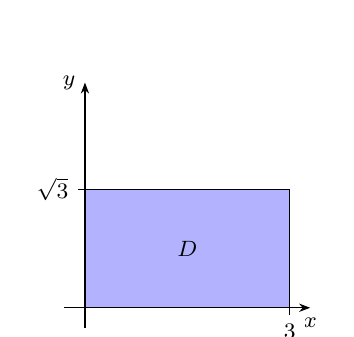
\begin{tikzpicture}[scale=1.3, baseline=(X.base)]
  \def\scale{1.3}
  \node at (0,0) (X) {};

  \drawaxes{0}{0}{2}{2}

  \draw[integration domain] (0,0) |- (2,1.155) |- cycle;

  \drawxlabels{2/3}
  \drawylabels{1.155/\sqrt{3}}

  \node at (1,.575) {$D$};
\end{tikzpicture}
&
\begin{tikzpicture}[scale=0.8666, baseline=(X.base)]
  \def\scale{0.8666}
  \node at (0,-1) (X) {};

  \drawxlabels{1/1, 3/3}
  \drawylabels{{ln(3)}/\ln 3}
  \drawaxes{0}{-1}{3}{2}

  \clip (0,-1) rectangle (3,2);

  \draw[integration domain]
    plot[parametric, domain=1:3, samples=100] function {t, log(t)}
    |- cycle;
    
  \draw[dashed]
    plot[parametric, domain=0.01:1, samples=100] function {t, log(t)};

  \draw[dotted] (0,{ln(3)}) -- (3,{ln(3)});

  \node at (2.3,0.3) {$D$};
\end{tikzpicture}
&
\begin{tikzpicture}[scale=2.6, baseline=(X.base)]
  \def\scale{2.6}
  \node at (0,0) (X) {};

  \drawylabels{1/1}
  \drawaxes{0}{0}{1}{1}
  \drawxlabels{0.785/\frac{\pi}4}


  \clip (0,0) rectangle (1,1);

  \draw[integration domain]
    plot[parametric, domain=0:1, samples=100] function {atan(t), t}
    |- cycle;

  \draw[dotted] (0,1) -- (0.785,1);

  \node at (.6,.3) {$D$};
\end{tikzpicture}
&
\begin{tikzpicture}[scale=0.8666, baseline=(X.base)]
  \def\scale{0.8666}
  \node at (0,-1.5) (X) {};

  \drawaxes{-1.5}{-1.5}{1.5}{1.5}
  \clip (-1.5,-1.5) rectangle (1.5,1.5);

  \draw[integration domain]
    plot[parametric, domain=-1.414:1.414, samples=100] function {t**2-1, t}
    -- cycle;

  \draw[dotted] (0,-1.414) -- (1,-1.414)
                (0,1.414) -- (1,1.414);

  \drawxlabels[nofill]{-1/-1,1/1}
  \drawylabels{-1.414/-\sqrt{2}, 1.414/\sqrt{2}}

  \node at (0,0) {$D$};
\end{tikzpicture}
\\
(a) & (b) & (c) & (d)
\end{figuretable}
\end{center}

\begin{enumerate}
\item
$\int_0^3 \int_0^{\sqrt{3}} f(x,y) \ud y \ud x
= \int_0^{\sqrt 3} \int_0^{3} f(x,y) \ud x \ud y$
\item
$\int_1^3 \int_0^{\ln x} f(x,y) \ud y \ud x
= \int_0^{\ln 3} \int_{e^y}^3 f(x,y) \ud x \ud y$
\item
$\int_0^1 \int_{\arctan y}^{\pi/4} f(x,y) \ud x \ud y
= \int_0^{\pi/4} \int_0^{\tan x} f(x,y) \ud y \ud x$
\item
$\int_{-\sqrt 2}^{\sqrt 2} \int_{y^2-1}^1 f(x,y) \ud x \ud y
= \int_{-1}^1 \int_{-\sqrt{x+1}}^{\sqrt{x+1}} f(x,y) \ud y \ud x$
\end{enumerate}
\end{solution}

\begin{question}
\SetQuestionProperties{source = {Ex. 17, 19, 20; MW, III.17.2}}
Sketch the region, interchange the order of integration and evaluate the integral.
\begin{tasks}(3)
\task
$\displaystyle \int_0^1 \int_x^1 xy \ud y \ud x$.
\task
$\displaystyle \int_0^1 \int_{1-y}^1 (x+y^2) \ud x \ud y$.
\task
$\displaystyle \int_1^4 \int_1^{\sqrt{x}} \left(x^2 + y^2\right) \ud y \ud x$.
\end{tasks}
\end{question}

\begin{solution} 
The regions are shown in the figures below.

\begin{center}
\begin{tabular}{ccc}
% Triangle (0,0) - (1,0) - (1,1)
\begin{tikzpicture}[scale=3.75, baseline=0]
  \def\scale{3.75}

  \drawaxes{0}{0}{1}{1}
  \drawxlabels{1/1}
  \drawylabels{1/1}

  \draw[black,integration domain] (0,0) -- (1,0) -- (1,1) -- cycle;
  \node[above left] at (0.75, 0.75) {$y=x$};

  \draw[dotted] (0,1) -- (1,1);

  \node at (0.66,.33) {$D$};
\end{tikzpicture}
&
% Triangle (1,0) - (1,1) - (0,1)
\begin{tikzpicture}[scale=3.75, baseline=0]
  \def\scale{3.75}

  \drawaxes{0}{0}{1}{1}
  \drawxlabels{1/1}
  \drawylabels{1/1}

  \draw[integration domain] (1,0) -- (1,1) -- (0,1) -- cycle;
  \node[below left, align=left] at (0.625, 0.375) {$x=1-y$};

  \node at (0.66,.66) {$D$};
\end{tikzpicture}
&
% Area between y=1, y=sqrt(x) and 1<x<4.
\begin{tikzpicture}[scale=0.9375, baseline=(BL)]
  \def\scale{0.9375}
  \coordinate (BL) at (0,-1);
  \coordinate (TR) at (4,3);

  \drawaxes{0}{-1}{4}{3}
  \drawxlabels{1/1, 4/4}
  \drawylabels{1/1, 2/2}

  \draw[dashed]
    plot[domain=0:1, samples=100, smooth] function {sqrt(x)};

  \draw[integration domain, smooth]
    plot[domain=1:4] function {sqrt(x)} |- cycle;
  \draw[dotted] (0,2) -- (4,2)
                (4,0) -- (4,1)
                (1,0) |- (0,1);

  \node[above] at (4,2) {$y=\sqrt{x}$};
  \node at (3,1.4) {$D$};
\end{tikzpicture}
\\
(a) & (b) & (c)
\end{tabular}
\end{center}

\begin{enumerate}
\item
We can write the domain as
\begin{align*}
D &= \left\{ (x,y) \,:\, 0 \leq x \leq 1\,,\; x \leq y \leq 1 \right\} \\
&= \left\{ (x,y) \,:\, 0 \leq y \leq 1\,,\; 0 \leq x \leq y \right\}\,.
\end{align*}
The integral then becomes
\[
\int_0^1 \int_x^1 xy \ud y \ud x = \int_0^1 \int_0^y xy \ud x \ud y
\]
We evaluate the latter integral
\begin{align*}
\int_0^1 \int_0^y xy \ud x \ud y
&= \int_0^1 \frac 12 x^2 y\bigg|_{x=0}^y \ud y
= \int_0^1 \frac 12 y^3 \ud y = \frac 18\,.
\end{align*}

\item
We can write the domain as
\begin{align*}
D &= \left\{ (x,y) \,:\, 0 \leq y \leq 1\,,\; 1-y \leq x \leq 1 \right\} \\
&= \left\{ (x,y) \,:\, 0 \leq x \leq 1\,,\; 1-x \leq y \leq 1 \right\}\,.
\end{align*}
The integral then becomes
\[
\int_0^1 \int_{1-y}^1 \left(x+y^2\right) \ud x \ud y = \int_0^1 \int_{1-x}^1 \left(x+y^2\right) \ud y \ud x \,.
\]
We evaluate the latter integral
\begin{align*}
\int_0^1 \int_{1-x}^1 \left(x+y^2\right) \ud y \ud x
&= \int_0^1 xy + \frac 13 y^3 \bigg|_{y=1-x}^1 \ud x
= \int_0^1 x^2 + \frac 13 - \frac 13 \left(1 - x\right)^3 \ud x \\
&= \frac 13 x^3 + \frac 13 x + \frac 1{12} \left(1-x\right)^4 \bigg|_{x=0}^1
= \frac 7{12}\,.
\end{align*}

\item
We can write the domain as
\begin{align*}
D &= \left\{ (x,y) \,:\, 1 \leq y \leq 4\,,\; 1 \leq y \leq \sqrt x \right\} \\
&= \left\{ (x,y) \,:\, 1 \leq y \leq 2\,,\; y^2 \leq x \leq 4 \right\}\,.
\end{align*}
The integral then becomes
\[
\int_1^4 \int_1^{\sqrt{x}} \left(x^2 + y^2\right) \ud y \ud x
= \int_1^2 \int_{y^2}^4 \left(x^2 + y^2 \right) \ud x \ud y\,.
\]
We evaluate the latter integral
\begin{align*}
\int_1^2 \int_{y^2}^4 \left(x^2 + y^2 \right) \ud x \ud y
&= \int_1^2 \frac 13 x^3 + y^2 x \bigg|_{x=y^2}^4 \ud y
= \int_1^2 \frac{64}3 - \frac 13 y^6 + 4y^2 - y^4 \ud y \\
&= \frac{64}{3} y - \frac 1{21}y^7 + \frac 43 y^3 - \frac 15 y^5 \bigg|_{y=1}^2
= \frac{1934}{105}\,.
\end{align*}
\end{enumerate}
\end{solution}

\begin{question}
\SetQuestionProperties{source = {MA2815 Exams, 2015}}
Evaluate the following integrals.
\begin{tasks}(2)
\task
$\int_{-1}^1 \int_1^2 \frac{x \tan^2 y}{1 + \ln y} \ud y \ud x$
\task
$\int_0^1 \int_{2x}^2 e^{-y^2} \ud y \ud x$
\task
$\int_0^2 \int_{y/2}^1 \cos\left(x^2\right) \ud x\ud y$
\task
$\int_0^1 \int_{\sqrt[3]{y}}^1 \sqrt{x^4+1} \ud x \ud y$
\task
$\int_0^2 \int_{y/2}^1 y \cos (x^3 - 1) \ud x \ud y$
\task
$\int_0^{\pi/2} \int_x^{\pi/2} \frac{\sin y}{y} \ud y \ud x$
\end{tasks}
\end{question}

\begin{solution}
\begin{center}
\begin{figuretable}{4}
\begin{tikzpicture}[scale=1.3, baseline=(X.base)]
  \def\scale{1.3}
  \node at (0,0) (X) {};

  \drawxlabels{1/1}
  \drawylabels{2/2}

  \drawaxes{0}{0}{2}{2}

  \draw[integration domain] (0,0) -- (1,2) -| cycle;

  \draw[dotted] (1,0) -- (1,2);

  \node at (0.333, 1.333) {$D$};
\end{tikzpicture}
&
\begin{tikzpicture}[scale=1.3, baseline=(X.base)]
  \def\scale{1.3}
  \node at (0,0) (X) {};

  \drawxlabels{1/1}
  \drawylabels{2/2}

  \drawaxes{0}{0}{2}{2}

  \draw[integration domain] (0,0) -- (1,2) |- cycle;

  \draw[dotted] (0,2) -- (1,2);

  \node at (0.666, 0.666) {$D$};
\end{tikzpicture}
&
\begin{tikzpicture}[scale=2.6, baseline=(X.base)]
  \def\scale{2.6}
  \node at (0,0) (X) {};

  \drawylabels{1/1}
  \drawxlabels{1/1}
  \drawaxes{0}{0}{1}{1}

  \clip (0,0) rectangle (1,1);

  \draw[integration domain]
    plot[parametric, domain=0:1, samples=100] function {t, t**3}
    |- cycle;

  \draw[dotted] (0,1) -- (1,1);

  \node at (.8,.3) {$D$};
\end{tikzpicture}
&
\begin{tikzpicture}[scale=2.6, baseline=(X.base)]
  \def\scale{2.6}
  \node at (0,0) (X) {};

  \node[left] at (0,.95) {$\textstyle\frac{\pi}2$};
  \node[below] at (1,0) {$\textstyle\frac{\pi}2$};
  \drawaxes{0}{0}{1}{1}
  \clip (0,0) rectangle (1,1);

  \draw[integration domain]
    (0,0) -- (1,1) -- (0,1) -- cycle;

  \draw[dotted] (1,0) -- (1,1);

  \node at (0.333,0.666) {$D$};
\end{tikzpicture}
\\
(b) & (c) \& (e) & (d) & (f)
\end{figuretable}
\end{center}
\begin{enumerate}
\item
\begin{alignenum}
\int_{-1}^1 \int_1^2 \frac{x \tan^2 y}{1 + \ln y} \ud y \ud x
= \int_1^2 \int_{-1}^1 \frac{x \tan^2 y}{1 + \ln y} \ud x \ud y
= \int_1^2 \frac 12 x^2 \cdot \frac{\tan^2 y}{1 + \ln y} \bigg|_{x=-1}^1 \ud y
= 0\,.
\end{alignenum}
\item
\begin{alignenum}
\int_0^1 \int_{2x}^2 e^{-y^2} \ud y \ud x
&= \int_0^2 \int_0^{y/2} e^{-y^2} \ud x \ud y
= \int_0^2 e^{-y^2} x \bigg|_{x=0}^{y/2} \ud y
= \int_0^2 e^{-y^2} \frac y2 \ud y \\
&= -\frac 14 e^{-y^2} \bigg|_{y=0}^2
= \frac 14 \left( 1 - e^{-4}\right)\,.
\end{alignenum}
% The region of integration can be expressed as
% \[
% \{ (x,y) \,:\, 0 \leq x \leq 1,\, 2x \leq y \leq 2 \}
% = \left\{ (x,y) \,:\, 0 \leq y \leq 2,\, 0 \leq x \leq \frac y2 \right\}\,.
% \]
% Interchanging the order of integration leads to
% \[
% I = \int_0^2 \int_0^{y/2} e^{-y^2} \ud x \ud y\,.
% \]
% The first integration is simple
% \[
% I = \int_0^2 e^{-y^2} x \bigg|_{x=0}^{y/2} \ud x = \int_0^2 e^{-y^2} \frac y2 \ud x
% \]
% Now we are also able to perform the $y$-integration
% \[
% I = -\frac 14 \int_0^2 -2y e^{-y^2} \ud y
% = -\frac 14 e^{-y^2} \bigg|_{y=0}^2 = \frac 14 \left( 1 - e^{-4}\right)\,.
% \]
\item
\begin{alignenum}
\int_0^2 \int_{y/2}^1 \cos\left(x^2\right) \ud x\ud y
&= \int_0^1 \int_0^{2x} \cos\left(x^2\right) \ud y \ud x
= \int_0^1 \cos\left( x^2 \right) y \bigg|_{y=0}^{2x} \ud x \\
&= \int_0^1 2x \cos\left(x^2\right) \ud x
= \sin\left(x^2\right) \bigg|_{x=0}^1 = \sin 1\,.
\end{alignenum}
% The region of integration can be expressed as
% \[
% \left\{ (x,y) \,:\, 0 \leq y \leq 2,\, \frac y2 \leq x \leq 1 \right\}
% = \{ (x,y) \,:\, 0 \leq x \leq 1 ,\, 0 \leq y \leq 2x \}\,.
% \]
% Interchanging the order of integration leads to
% \[
% I = \int_0^1 \int_0^{2x} \cos\left(x^2\right) \ud y \ud x\,.
% \]
% The first integration is simple
% \[
% I = \int_0^1 \cos\left( x^2 \right) y \bigg|_{y=0}^{2x} \ud x
% = \int_0^1 2x \cos\left(x^2\right) \ud x\,.
% \]
% Now we are also able to perform the $x$-integration
% \[
% I = \sin\left(x^2\right) \bigg|_{x=0}^1 = \sin 1\,.
% \]
\item
\begin{alignenum}
\int_0^1 \int_{\sqrt[3]{y}}^1 \sqrt{x^4+1} \ud x \ud y
&= \int_0^1 \int_0^{x^3} \sqrt{x^4+1} \ud y \ud x
= \int_0^1 y \sqrt{x^4 + 1} \,\bigg|_{y=0}^{x^3} \ud x \\
&= \int_0^1 x^3 \sqrt{x^4 + 1} \ud x
= \frac 16 \left(x^4 + 1\right)^{3/2} \bigg|_{x=0}^1
= \frac 16 \left(2\sqrt{2} - 1\right)\,.
\end{alignenum}
\item
\begin{alignenum}
\int_0^2 \int_{y/2}^1 y \cos \left(x^3 - 1 \right) \ud x \ud y
&= \int_0^1 \int_0^{2x} y \cos \left(x^3 - 1 \right) \ud y \ud x
= \int_0^1 \frac 12 y^2 \cos \left( x^3 - 1 \right) \bigg|_{y=0}^{2x} \ud x \\
&= \int_0^1 2x^2 \cos \left(x^3 - 1 \right) \ud x
= \frac 23 \sin \left(x^3 - 1 \right) \bigg|_{x=0}^1
= \frac 23 \sin 1\,.
\end{alignenum}
\item
\begin{alignenum}
\int_0^{\pi/2} \int_x^{\pi/2} \frac{\sin y}{y} \ud y \ud x
&= \int_0^{\pi/2} \int_0^{y} \frac{\sin y}{y} \ud x \ud y
= \int_0^{\pi/2} x \cdot \frac{\sin y}{y} \bigg|_{x=0}^y \ud y \\
&= \int_0^{\pi/2} \sin y \ud y = 1\,.
\end{alignenum}
\end{enumerate}
\end{solution}

\begin{question}
\SetQuestionProperties{difficulty = {*}}
Evaluate the iterated integral
\[
\int_0^2 \int_0^{2\sqrt{4-x^2}} \left( 4-x^2 - \frac 14 y^2\right) \ud y \ud x\,.
\]
\begin{hint*}
After performing the integration with respect to $y$, use a change of coordinates to transform the square roots from $\sqrt{4-x^2}$ to $\sqrt{1-u^2}$. Then use the trigonometric subsitution. To evaluate the resulting integral you will need to apply the half-angle formula twice.
\end{hint*}
\end{question}

\begin{solution}
We do the calculations step by step.
\begin{align*}
\int_0^2 \int_0^{2\sqrt{4-x^2}} \left( 4-x^2 - \frac 14 y^2\right) \ud y \ud x 
&= \int_0^2 8 \sqrt{4-x^2} - 2x^2 \sqrt{4-x^2} - \frac 8{12} \left(\sqrt{4-x^2}\right)^3 \ud x \\
&= \int_0^2 \frac 43 \left( \sqrt{4-x^2} \right)^3 \ud x
= \int_0^2 \frac {32}3 \left( \sqrt{1-\frac{x^2}4} \right)^3 \ud x\,.
\end{align*}
Now make the substitution $\frac x2 = u$ with $\ud x = 2 \ud u$. We obtain
\[
\int_0^2 \frac {32}3 \left( \sqrt{1-\frac{x^2}4} \right)^3 \ud x = 2 \int_0^1 \frac {32}3 \left( \sqrt{1-u^2} \right)^3 \ud u\,.
\]
Next we use the trigonometric substitution $u = \sin t$ with $\ud u = \cos t \ud t$. This leads to
\[
2 \int_0^1 \frac {32}3 \left( \sqrt{1-u^2} \right)^3 \ud u =
2 \int_0^{\pi/2} \frac {32}3 \left( \sqrt{1-\sin^2 t} \right)^3 \cos t \ud u =
\frac{64}3 \int_0^{\pi/2}  \cos^4 t \ud u\,.
\]
To evaluate this integral we use the half-angle formula twice to get
\begin{align*}
\cos^4 t &= \left( \frac{1 + \cos 2t}2 \right)^2 = \frac 14 + \frac 12 \cos 2t + \frac 14 \cos^2 2t \\
&= \frac 14 + \frac 12 \cos 2t + \frac 14 \frac{1 + \cos 4t}2 = \frac 38 + \frac 12 \cos 2t + \frac 18 \cos 4t\,.
\end{align*}
This is now easy to integrate
\[
\frac{64}3 \int_0^{\pi/2} \frac 38 + \frac 12 \cos 2t + \frac 18 \cos 4t \ud u =
\frac{64}3 \left. \left( \frac 38 t + \frac 14 \sin 2t + \frac 1{32} \sin 4t \right) \right|_{t=0}^{\pi/2} = 4 \pi\,.
\]
\end{solution}

\begin{question}
\SetQuestionProperties{difficulty = {*}}
\SetQuestionProperties{source = {Ex. 28; MW, III.17.2}}
Prove
$\int_0^x \int_0^t f(u) \ud u \ud t = \int_0^x (x-u) f(u) \ud u\,.$
\end{question}

\begin{solution}
\begin{adjustbox}{valign=T,raise=\strutheight,minipage={\linewidth}}
  \begin{wrapfigure}{r}{0.35\textwidth}
    \centering
\begin{tikzpicture}[scale=2.6, baseline=(X.base)]
  \def\scale{2.6}
  \node at (0,0) (X) {};

  \drawxaxis[$t$]{0}{1}
  \drawyaxis[$u$]{0}{1}
  \drawxlabels{1/x}
  \drawylabels{1/x}
  \clip (0,0) rectangle (1,1);

  \draw[integration domain]
    (0,0) -- (1,1) -- (0,1) -- cycle;

  \draw[dotted] (1,0) -- (1,1);

  \node at (0.333,0.666) {$D$};
\end{tikzpicture}
\end{wrapfigure}
\strut{}
Treating $x$ as a constant, we change the order of integration
\begin{align*}
\int_0^x \int_0^t f(u) \ud u \ud t 
&= \int_0^x \int_u^x f(u) \ud t \ud u \\
&= \int_0^x f(u) \left( \int_0^x 1 \ud t \right) \ud u \\
&= \int_0^x (x-u) f(u) \ud u\,.
\end{align*}
\end{adjustbox}
\end{solution}


%%% Local Variables:
%%% mode: latex
%%% TeX-master: "problems"
%%% End:

\ifthenelse{\boolean{sectionnewpage}}{\newpage}{}

\section{Polar Coordinates and the Change of Coordinates}
\begin{question}
Sketch the following regions in polar coordinates.
\begin{center}
\begin{figuretable}{3}
\begin{tikzpicture}[scale=1.875, baseline=(X.base)]
  \def\scale{1.875}
  \node at (0,-1) (X) {};

  \drawaxes{-1}{-1}{1}{1}

  \node[below right] at (45:.4) {$y=x$};
  \node[below left] at (135:.4) {$y=-x$};

  \draw[dashed] (0,0) circle (1);
  \draw[dashed] (45:1) -- (1,1);
  \draw[dashed] (135:1) -- (-1,1);

  \draw[integration domain] (0,0) -- (45:1)
    arc[radius=1, start angle=45, end angle=135] -- cycle;

  \drawxlabels[fill]{1/1}
\end{tikzpicture}
&
\begin{tikzpicture}[scale=1.875, baseline=(X.base)]
  \def\scale{1.875}
  \node at (0,-1) (X) {};

  \drawaxes{-1}{-1}{1}{1}

  \draw[dashed] (0,0) circle (1);
  \draw[dashed] (0,0) circle (0.5);

  \draw[integration domain] (0,0.5) -- (0,1)
    arc[radius=1, start angle=90, end angle=-90] -- (0,-.5)
    arc[radius=.5, start angle=-90, end angle=90];

  \drawylabels{.5/\frac{1}{2}, 1/1}
\end{tikzpicture}
&
\begin{tikzpicture}[scale=1.875, baseline=(X.base)]
  \def\scale{1.875}
  \node at (0,-1) (X) {};

  \drawaxes{-1}{-1}{1}{1}

  \draw[integration domain]
    plot[parametric, domain=0:2*3.1416, samples=100]
      function {sin(t)**2*cos(t), sin(t)**3};

  \node[right] at (75:1) {$r=\sin^2 \th$};
\end{tikzpicture}
\\
(a) & (b) & (c)
\end{figuretable}
\end{center}
\end{question}

\begin{solution}
In polar coordinates the domains are as follows.
\begin{center}
\begin{figuretable}{3}
\begin{tikzpicture}[scale=1.875, baseline=(X.base)]
  \def\scale{1.875}
  \node at (0,0) (X) {};

  \drawxaxis[$\th$]{0}{2};
  \drawyaxis[$r$]{-.08}{1.08};

  \draw[integration domain] (0.5,0) -| (1.5,1) -| cycle;

  \draw[dotted] (0,1) -- (0.5,1);

  \drawylabels{1/1}
  \drawxlabels{.5/\frac{\pi}{4}, 1.5/\frac{3\pi}4}
\end{tikzpicture}
&
\begin{tikzpicture}[scale=1.875, baseline=(X.base)]
  \def\scale{1.875}
  \node at (0,0) (X) {};

  \drawxaxis[$\th$]{-1}{1};
  \drawyaxis[$r$]{-.08}{1.08};

  \draw[integration domain] (-1,0.5) -| (1,1) -| cycle;

  \draw[dotted] (-1,0) -- (-1,0.5)
                (1,0) -- (1,0.5);

  \drawylabels[nofill]{.5/\frac{1}{2}, 1/1}
  \drawxlabels{-1/-\pi, 1/\pi}
\end{tikzpicture}
&
\begin{tikzpicture}[scale=1.875, baseline=(X.base)]
  \def\scale{1.875}
  \node at (0,0) (X) {};

  \drawxaxis[$\th$]{-1}{1};
  \drawyaxis[$r$]{-.08}{1.08};

  \draw[integration domain]
    plot[parametric, domain=-1:1, samples=100]
      function {t, sin(t*pi)**2} -- cycle;

  %\node[above] at (0.5,1) {$r=\sin^2 \th$};

  \drawxlabels{-1/-\pi, 1/\pi}
\end{tikzpicture}
\\
(a) & (b) & (c)
\end{figuretable}
\end{center}
\end{solution}

\begin{question}
Sketch the following regions in cartesian coordinates.
\begin{center}
\begin{figuretable}{3}
\begin{tikzpicture}[scale=1.875, baseline=(X.base)]
  \def\scale{1.875}
  \node at (0,0) (X) {};

  \drawxaxis[$\th$]{-1}{1};
  \drawyaxis[$r$]{-.08}{1.08};

  \draw[integration domain] (-.8,0) |- (.8,1) |- cycle;

  \drawxlabels{-.8/\frac{-\pi}{4}, .8/\frac{3\pi}{4}}
  \drawylabels[nofill]{1/1}
\end{tikzpicture}
&
\begin{tikzpicture}[scale=1.875, baseline=(X.base)]
  \def\scale{1.875}
  \node at (0,0) (X) {};

  \drawxaxis[$\th$]{0}{2};
  \drawyaxis[$r$]{-.08}{1.08};

  \draw[integration domain] (0.5,0.25) -| (2,1) -| cycle;

  \draw[dotted] (0.5,0) -- (0.5,0.25)
                (2,0) -- (2,0.25)
                (0,0.25) -- (0.5,0.25)
                (0,1) -- (0.5,1);

  \drawylabels{.25/\frac{1}{4}, 1/1}
  \drawxlabels{.5/\frac{\pi}{4}, 2/\pi}
\end{tikzpicture}
&
\begin{tikzpicture}[scale=1.875, baseline=(X.base)]
  \def\scale{1.875}
  \node at (0,0) (X) {};

  \drawxaxis[$\th$]{-1}{1};
  \drawyaxis[$r$]{-.08}{1.08};

  \draw[integration domain]
    plot[parametric, domain=-1:1, samples=100]
      function {t, 0.5*(1+cos(pi*t))} -- cycle;

  \node[right] at (0.3,0.8) {$r=1 + \cos \th$};

  \drawxlabels{-1/-\pi, 1/\pi}
\end{tikzpicture}
\\
(a) & (b) & (c)
\end{figuretable}
\end{center}
\end{question}

\begin{solution}
In cartesian coordinates the domains are as follows.
\begin{center}
\begin{figuretable}{3}
\begin{tikzpicture}[scale=1.875, baseline=(X.base)]
  \def\scale{1.875}
  \node at (0,-1) (X) {};

  \drawaxes{-1}{-1}{1}{1}

  %\node[left] at (-55:.8) {$\th=-\frac \pi 4$};
  %\node[left] at (145:.4) {$\th=\frac {3\pi}4$};

  \draw[dashed] (0,0) circle (1);
  \draw[dashed] (-45:1) -- (1,-1);
  \draw[dashed] (135:1) -- (-1,1);

  \draw[integration domain] (0,0) -- (-45:1)
    arc[radius=1, start angle=-45, end angle=135] -- cycle;

  \drawxlabels[nofill]{1/1}
\end{tikzpicture}
&
\begin{tikzpicture}[scale=1.875, baseline=(X.base)]
  \def\scale{1.875}
  \node at (0,-1) (X) {};

  \drawaxes{-1}{-1}{1}{1}

  \draw[dashed] (0,0) circle (1);
  \draw[dashed] (0,0) circle (0.25);

  \draw[integration domain] (45:0.25) -- (45:1)
    arc[radius=1, start angle=45, end angle=180] -- (-0.25,0)
    arc[radius=.25, start angle=180, end angle=45];

  \drawxlabels{.25/\frac{1}{4}, 1/1}
\end{tikzpicture}
&
\begin{tikzpicture}[scale=1.25, baseline=(X.base)]
  \def\scale{1.25}
  \node at (0,-1.5) (X) {};

  \drawaxes{-1}{-1.5}{2}{1.5};

  \draw[integration domain]
    plot[parametric, domain=0:2*pi, samples=100]
      function {(1+cos(t))*cos(t), (1+cos(t))*sin(t)};
\end{tikzpicture}
\\
(a) & (b) & (c)
\end{figuretable}
\end{center}
\end{solution}

\begin{question}
\SetQuestionProperties{source={Thomas 12th, 15.4}}
Find the limits for integrating $f(x,y)$ over the region $D$ using polar coordinates.
\begin{center}
\begin{tabu} to \linewidth {*3{X[1,c]}}
\begin{tikzpicture}[scale=1.25, baseline=(X.base)]
  \def\scale{1.25}
  \node at (0,-1.5) (X) {};

  \drawaxes{-1}{-1.5}{2}{1.5};

  \draw[dashed] (0,1) arc[radius=1, start angle=90, end angle=270];
  \draw[dashed] plot[parametric, domain=3.1416/2:3*3.1416/2, samples=100]
          function {(1+cos(t))*cos(t), (1+cos(t))*sin(t)};

  \draw[integration domain]
    plot[parametric, domain=-3.1416/2:3.1416/2, samples=100]
      function {(1+cos(t))*cos(t), (1+cos(t))*sin(t)}
    arc[radius=1, start angle=90, end angle=-90];

  \node at (1.5,0) {$D$};

  \node[above right] at (60:1.5) {$r=1+\cos \th$};
  \node[above left] at (120:1) {$r=1$};
\end{tikzpicture}
&
\begin{tikzpicture}[scale=1.875, baseline=(X.base)]
  \def\scale{1.875}
  \node at (0,0) (X) {};

  \drawaxes{0}{0}{2}{2}

  \draw[dashed] (45:2) arc[radius=2, start angle=45, end angle=0];
  
  \draw[integration domain] (0,2) 
    arc[radius=2, start angle=90, end angle=45] -| cycle;

  \node at (0.4,1.7) {$D$};

  \drawxlabels{2/2};
  \drawylabels{2/2, 1.414/\sqrt{2}};

\end{tikzpicture}
&
\begin{tikzpicture}[scale=1.875, baseline=(X.base)]
  \def\scale{1.875}
  \node at (0,0) (X) {};

  \drawaxes{0}{0}{2}{2}

  \draw[integration domain]
    (0,0) -- ({sqrt(3)},1) |- cycle;

  \draw[dashed] (0,1) -- ({sqrt(3)},1);

  \node at (1.2,0.4) {$D$};

  \drawxlabels{1.732/\sqrt{3}}
  \drawylabels{1/1};
\end{tikzpicture}
\\
(a) & (b) & (c)
\end{tabu}
\end{center}
\end{question}

\begin{solution}
\begin{enumerate}
\item
The integral is
\[
\int_{-\pi/2}^{\pi/2} \int_1^{1+\cos \th} f(r,\th) r \ud r \ud \th\,.
\]
\item
The line $y=\sqrt{2}$ in polar coordinates is given by
\[
r \sin \th = \sqrt{2}
\quad\Leftrightarrow\quad
r = \frac{\sqrt 2}{\sin \th}\,.
\]
It intersects the circle in the point $\left(\sqrt 2, \sqrt 2\right)$, which corresponds to $\th = \frac \pi 4$. Therefore the integral is
\[
\int_{\pi/4}^{\pi/2} \int_{\sqrt 2/\sin \th}^2 f(r,\th) r \ud r \ud \th\,.
\]
\item
The line $x=\sqrt{3}$ in polar coordinates is given by
\[
r \cos \th = \sqrt 3
\quad\Leftrightarrow\quad
r = \frac{\sqrt 3}{\cos \th}\,,
\]
and the hypothenuse of the triangle has slope $\frac{1}{\sqrt 3}$, which corresponds to $\th=\frac \pi 6$. Therefore the integral is
\[
\int_0^{\pi/6} \int_0^{\sqrt 3/\cos \th} f(r,\th) r \ud r \ud \th\,.
\]
\end{enumerate}
\end{solution}

\begin{question}
Evaluate the given integrals using polar coordinates.
\begin{tasks}(1)
\task
$\iint_D 3x-y + 4 \ud x \ud y$, where $D$ is the region enclosed by the circle $x^2 + y^2 = 1$.
\task
$\iint_D 2x - y \ud x \ud y$, where $D$ is the region in the first quadrant enclosed by the circle $x^2 + y^2 = 4$ and the lines $x=0$ and $y=x$.
\task
$\iint_D x^2 y \ud x \ud y$, where $D$ is the top half of the disk with center the origin and radius $3$.
\task
$\iint_D \ln \left(x^2 + y^2\right) \ud x \ud y$, where $D$ is the region between the circles $x^2 + y^2 = 1$ and $x^2 + y^2 = 4$.
\end{tasks}
\end{question}

\begin{solution}
The domains of integration are shown below.
\begin{center}
\begin{figuretable}{4}
\begin{tikzpicture}[scale=1.3, baseline=(X.base)]
  \def\scale{1.3}
  \node at (0,-1) (X) {};

  \drawaxes{-1}{-1}{1}{1}

  \draw[integration domain] (0,0) circle (1);

  \node at (0,0) {$D$};
  \node[right] at (60:1.05) {$r=1$};
\end{tikzpicture}
&
\begin{tikzpicture}[scale=1.3, baseline=(X.base)]
  \def\scale{1.3}
  \node at (0,0) (X) {};

  \drawaxes{0}{0}{2}{2}
  \drawxlabels[nofill]{2/2};
  \clip (0,0) rectangle (2,2);

  \draw[integration domain] (0,0) -- (2,0)
    arc[radius=2, start angle=0, end angle=45] 
    -- cycle;

  \draw[dashed] (45:2) -- (45:4);
  \draw[dashed] 
    (45:2) arc[radius=2, start angle=45, end angle=90];

  \node at (1.2,0.5) {$D$};
  \node[left] at (45:1.6) {$y=x$};
\end{tikzpicture}
&
\begin{tikzpicture}[scale=1.3, baseline=(X.base)]
  \def\scale{1.3}
  \node at (0,-1) (X) {};

  \draw[dashed]
    (1,0) arc[radius=1, start angle=0, end angle=-180];

  \drawxlabels{1/1}
  \drawaxes{-1}{-1}{1}{1}

  \draw[integration domain] 
    (1,0) arc[radius=1, start angle=0, end angle=180] -- cycle;

  \node at (0,0.4) {$D$};
\end{tikzpicture}
&
\begin{tikzpicture}[scale=1.3, baseline=(X.base)]
  \def\scale{1.3}
  \node at (0,-1) (X) {};

  \drawaxes{-1}{-1}{1}{1}

  \draw[integration domain, even odd rule]
    (0,0) circle (1)
    (0,0) circle (0.5);

  \node at (45:0.75) {$D$};
  \node[left] at (20:0.5) {$r=1$};
  \node[right] at (60:1.05) {$r=2$};
\end{tikzpicture}
\\
(a) & (b) & (c) & (d)
\end{figuretable}
\end{center}

\begin{enumerate}
\item
\begin{alignenum}
\iint_D 3x-y + 4 \ud x \ud y 
&= \int_0^1 \int_0^{2\pi} \left( 3r \cos \th - r \sin \th + 4 \right) r \ud \th \ud r \\
&= \int_0^1 3r^2 \sin \th + r^2 \cos \th + 4r\th \bigg|_{\th=0}^{2\pi} \ud r 
= \int_0^1 8\pi r \ud r = 4\pi\,.
\end{alignenum}
\item
\begin{alignenum}
\iint_D 2x-y \ud x \ud y
&= \int_0^2 \int_0^{\pi/4} \left( 2r \cos \th - r \sin \th \right) r \ud \th \ud r \\
&= \int_0^2 2r^2 \sin \th + r^2 \cos \th \bigg|_{\th=0}^{\pi/4} \ud r
= \int_0^2 \left( \frac 32 \sqrt{2} - 1\right) r^2 \ud r
= 4 \sqrt{2} - \frac 83 \,.
\end{alignenum}
\item
\begin{alignenum}
\iint_D x^2 y \ud x \ud y
&= \int_0^3 \int_0^\pi r^4 \cos^2 \th \sin \th \ud \th \ud r \\
&= \int_0^3 - \frac 13 r^4 \cos^3 \th \bigg|_{\th=0}^\pi \ud r
= \int_0^3 \frac 23 r^4 \ud r = \frac{162}{5}\,.
\end{alignenum}
\item
\begin{alignenum}
\iint_D \ln \left(x^2 + y^2 \right) \ud x \ud y
&= \int_1^2 \int_0^{2\pi} \ln\left(r^2\right) r \ud \th \ud r
= 2\pi \int_1^{\sqrt{2}} \frac 12 \ln u \ud u \\
&= \pi \left( u \ln u \bigg|_{u=1}^{\sqrt{2}} - \int_1^{\sqrt 2} 1 \ud u \right)
= \pi \left( \frac {\sqrt 2}2 \ln 2 + 1 - \sqrt 2 \right)\,.
\end{alignenum}
\end{enumerate}
\end{solution}

\begin{question}
Evaluate the given integrals.
\begin{tasks}(2)
\task
$\int_{-1}^1 \int_0^{\sqrt{1-x^2}} 1 \ud y \ud x$
\task
$\int_0^1 \int_0^{\sqrt{1-x^2}} \sqrt{x^2 + y^2} \ud y \ud x$
\task
$\int_0^{1/2} \int_{\sqrt{3}y}^{\sqrt{1-y^2}} y^2 \ud x \ud y$
\task
$\int_0^1 \int_x^{\sqrt{2-x^2}} x+2y \ud y \ud x$
\end{tasks}
\end{question}

\begin{solution}
The domains of integration are shown below.
\begin{center}
\begin{figuretable}{4}
\begin{tikzpicture}[scale=1.3, baseline=(X.base)]
  \def\scale{1.3}
  \node at (0,-1) (X) {};

  \draw[dashed]
    (1,0) arc[radius=1, start angle=0, end angle=-180];

  \drawxlabels{1/1}
  \drawaxes{-1}{-1}{1}{1}

  \draw[integration domain] 
    (1,0) arc[radius=1, start angle=0, end angle=180] -- cycle;

  \node at (0,0.4) {$D$};
\end{tikzpicture}
&
\begin{tikzpicture}[scale=1.3, baseline=(X.base)]
  \def\scale{1.3}
  \node at (0,0) (X) {};

  \draw[integration domain] (0,0) -- (2,0)
    arc[radius=2, start angle=0, end angle=90] 
    -- cycle;

  \drawaxes{0}{0}{2}{2}
  \drawxlabels[nofill]{2/1};

  \node at (45:1.33) {$D$};
\end{tikzpicture}
&
\begin{tikzpicture}[scale=1.3, baseline=(X.base)]
  \def\scale{1.3}
  \node at (0,0) (X) {};

  \drawaxes{0}{0}{2}{2}
  \drawxlabels[nofill]{2/1};
  \drawylabels{1/\textstyle\frac 12};
  \clip (0,0) rectangle (2,2);

  \draw[integration domain] (0,0) -- (2,0)
    arc[radius=2, start angle=0, end angle=30] 
    -- cycle;

  \draw[dashed] (30:2) -- (30:4);
  \draw[dashed] 
    (30:2) arc[radius=2, start angle=30, end angle=90];

  \draw[dotted] (0,1) -- (30:2);

  \node at (15:1.333) {$D$};
  \node[left] at (33:1.3) {$\textstyle \th=\frac \pi 6$};
\end{tikzpicture}
&
\begin{tikzpicture}[scale=1.3, baseline=(X.base)]
  \def\scale{1.3}
  \node at (0,0) (X) {};

  \drawaxes{0}{0}{2}{2}
  \drawxlabels[nofill]{1.414/1, 2/};
  \node[below] at (1.95,0) {$\sqrt 2$}; % Manual alignment

  \node[left] at (46:2.6) {$\textstyle\th=\frac \pi 4$};

  \clip (0,0) rectangle (2,2);

  \draw[integration domain] (0,0) -- (45:2)
    arc[radius=2, start angle=45, end angle=90] 
    -- cycle;

  \draw[dashed] (45:2) -- (45:4);
  \draw[dashed] 
    (0:2) arc[radius=2, start angle=0, end angle=45];

  \draw[dotted] (45:2)|-(0,0) -- (45:2);

  \node at (67.5:1.333) {$D$};
\end{tikzpicture}
\\
(a) & (b) & (c) & (d)
\end{figuretable}
\end{center}
We evaluate the integrals using polar coordinates.
\begin{enumerate}
\item
\begin{alignenum}
\int_{-1}^1 \int_0^{\sqrt{1-x^2}} 1 \ud y \ud x
&= \int_0^\pi \int_0^1 r \ud r \ud \th
= \int_0^\pi \frac 12 r^2 \bigg|_{r=0}^1 \ud \th = \frac \pi 2\,.
\end{alignenum}
\item
\begin{alignenum}
\int_{0}^1 \int_0^{\sqrt{1-x^2}} \sqrt{x^2 + y^2} \ud y \ud x
= \int_0^{\pi/2} \int_0^1 r^2 \ud r \ud \th
= \int_0^{\pi/2} \frac 13 r^3 \bigg|_{r=0}^1 \ud \th
= \frac \pi 6\,.
\end{alignenum}
\item
\begin{alignenum}
\int_{0}^{1/2} \int_{\sqrt 3 y}^{\sqrt{1-y^2}} y^2 \ud x \ud y
&= \int_0^{\pi/6} \int_0^1 r^3 \sin^2 \th \ud r \ud \th 
= \frac 14 \int_0^{\pi/6} \sin^2 \th \ud \th \\
&= \frac 18 \int_0^{\pi/6} 1 - \cos 2\th \ud \th
= \frac 18 \left( \th - \frac 12 \sin 2\th \right) \bigg|_{\th=0}^{\pi/6}
%= \frac \pi{48} - \frac 1{16} \sin \frac \pi 3 
= \frac \pi{48} - \frac 1{32}\,.
\end{alignenum}
\item
\begin{alignenum}
\int_0^1 \int_x^{\sqrt{2-x^2}} &x + 2y \ud y \ud x
= \int_{\pi/4}^{\pi/2} \int_0^{\sqrt 2} \left( r \cos \th + 2r \sin \th \right) 
\cdot r \ud r \ud \th \\
&= \int_{\pi/4}^{\pi/2} \frac 13 r^3 \left( \cos \th + 2 \sin \th \right)
\bigg|_{r=0}^{\sqrt 2} \ud \th
= \frac 23 \sqrt 2 \int_{\pi/4}^{\pi/2} \cos \th + 2 \sin \th \ud \th \\
&= \frac 23 \sqrt 2 \left( \sin \th - 2 \cos \th \right) \bigg|_{\th=\pi/4}^{\pi/2}
= \frac 23 \sqrt 2 \left( 1- \frac{\sqrt 2}2 + 2 \frac{\sqrt{2}}2 \right)
= \frac 23 \left(1 + \sqrt 2\right)\,.
\end{alignenum}
\end{enumerate}
\end{solution}

\begin{question}
\SetQuestionProperties{source={Ex. 27, 29, 30; Thomas 12th, 15.4}}
Find the following areas.
\begin{tasks}(1)
\task
The area enclosed by the positive $x$-axis and the spiral $r=\frac 32 \th$ with $0 \leq \th \leq 2\pi$. The area looks like a snail shell.
\task
The area enlosed by the cardioid $r = 1 + \cos \th$.
\task
The area cut from the first quadrant by the curve $r=2\sqrt{2-\sin 2\th}$.
\task
The area enclosed by one leaf of the rose $r = 12 \cos 3\th$.
\end{tasks}
\end{question}

\begin{solution}
The areas can be seen below.
\begin{center}
\begin{figuretable}{4}
\begin{tikzpicture}[scale=1.3, baseline=(X.base)]
  \def\scale{1.3}
  \node at (0,-1) (X) {};

  \drawaxes{-1}{-1}{1}{1}
 
  \clip (-1,-1) rectangle (1.1,1.1);

  \draw[integration domain] 
    plot[parametric, domain=0:2*pi, samples=100] 
      function {1.5*t*cos(t)/(3*pi), 1.5*t*sin(t)/(3*pi)}
    -- cycle;

  \draw[dashed]
    plot[parametric, domain=2*pi:2.5*pi, samples=100] 
      function {1.5*t*cos(t)/(3*pi), 1.5*t*sin(t)/(3*pi)};

  \node at (0.333,-0.33) {$D$};
  \node[above left] at (100:0.25) {$\textstyle r=\frac 32 \th$};
\end{tikzpicture}
&
\begin{tikzpicture}[scale=0.8666, baseline=(X.base)]
  \def\scale{0.8666}
  \node at (0,-1.5) (X) {};

  \drawaxes{-1}{-1.5}{2}{1.5};

  \draw[integration domain]
    plot[parametric, domain=0:2*pi, samples=100]
      function {(1+cos(t))*cos(t), (1+cos(t))*sin(t)};

  \node at (1,0) {$D$};

  \node[above right] at (80:1.3) {$r=1+\cos \th$};
\end{tikzpicture}
&

\begin{tikzpicture}[scale=0.3714, baseline=(X.base)]
  \def\scale{0.3714}
  \node at (0,-3.5) (X) {};

  \drawaxes{-3.5}{-3.5}{3.5}{3.5};

  \node[below right, fill=white] at (-3.5,-2.8) 
    {$r=2\sqrt{2-\sin 2\th}$};

  \draw[integration domain]
    plot[parametric, domain=0:2*pi, samples=100]
      function {2*sqrt(2-sin(2*t))*cos(t), 2*sqrt(2-sin(2*t))*sin(t)};

  \node at (0,0) {$D$};
\end{tikzpicture}
&
\begin{tikzpicture}[scale=1.3, baseline=(X.base)]
  \def\scale{1.3}
  \node at (0,-1) (X) {};

  \drawaxes{-1}{-1}{1}{1}

  \draw[integration domain]
    plot[parametric, domain=-pi/6:pi/6, samples=100]
      function {cos(3*t)*cos(t), cos(3*t)*sin(t)};

  \draw[dashed]
    plot[parametric, domain=pi/6:5*pi/6, samples=100]
      function {cos(3*t)*cos(t), cos(3*t)*sin(t)};

  \node at (0.6,0) {$D$};
  \node at (0.5,0.35) {$r=12 \cos 3\th$};
\end{tikzpicture}
\\
(a) & (b) & (c) & (d)
\end{figuretable}
\end{center}
We denote the area by $A$.
\begin{enumerate}
\item
\begin{alignenum}
A &= \int_0^{2\pi} \int_0^{3\th/2} r \ud r \ud \th
= \int_0^{2\pi} \frac 12 r^2 \bigg|_{r=0}^{3\th/2} \ud \th
= \int_0^{2\pi} \frac 98 \th^2 \ud \th
= 3\pi^3\,.
\end{alignenum}
\item
\begin{alignenum}
A &= \int_0^{2\pi} \int_0^{1 + \cos \th} r \ud r \ud \th
= \int_0^{2\pi} \frac 12 \left( 1 + \cos \th\right)^2 \ud \th
= \frac 12 \int_0^{2\pi} 1 + 2 \cos \th + \cos^2 \th \ud \th \\
&= \pi + \frac 14 \int_0^{2\pi} 1 + \cos 2\th \ud \th
= \frac {3\pi}2 + \frac 18 \sin 2\th \bigg|_{\th=0}^{2\pi} = \frac {3\pi}2\,.
\end{alignenum}
\item
\begin{alignenum}
A &= \int_0^{\pi 4} \int_0^{2\sqrt{2-\sin 2\th}} r \ud r \ud \th 
= \int_0^{\pi 4} \frac 12 \cdot 4 
\left( 2 - \sin 2\th \right) \ud \th
= \pi - \int_0^{\pi/4} 2 \sin 2 \th \ud \th \\
&= \pi + \cos 2 \th \bigg|_{\th=0}^{\pi/4}
= \pi - 1\,.
\end{alignenum}
\item
\begin{alignenum}
A &= \int_{-\pi/6}^{\pi/6} \int_0^{12 \cos 3\th} r \ud r \ud \th
= \int_{-\pi/6}^{\pi/6} \frac 12 r^2 \bigg|_{\th=0}^{12 \cos 3 \th} \ud \th
= 72 \int_{-\pi/6}^{\pi/6} \cos^2 3\th \ud \th \\
&= 36 \int_{-\pi/6}^{\pi/6} 1 - \cos 6 \th \ud \th
= 12\pi - 6 \sin 6\th \bigg|_{\th=-\pi/6}^{\pi/6} = 12 \pi\,.
\end{alignenum}
\end{enumerate}
\end{solution}

\begin{question}
\SetQuestionProperties{difficulty={*}}
Evaluate the following integrals using polar coordinates.
\begin{tasks}(1)
\task
$\iint_D \arctan \frac y x \ud x \ud y$;
$D = \{ (x,y)\,:\, 1 \leq x^2 + y^2 \leq 4,\, y \leq x \}$.
\task
$\iint_D \frac{x-y}{x+y} \ud x \ud y$; $D$ is the region enclosed by the lines $y=x$, $y=0$ and the circle $x^2 + y^2 = 1$ in the first quadrant.
\end{tasks}
\end{question}

\begin{solution}
\begin{enumerate}
\item
\begin{adjustbox}{valign=T,raise=\strutheight,minipage={\linewidth}}
  \begin{wrapfigure}{r}{0.35\textwidth}
    \centering
\begin{tikzpicture}[scale=1.875, baseline=(X.base)]
  \def\scale{1.875}
  \node at (0,-1) (X) {};

  \drawaxes{-1}{-1}{1}{1}

  \node[left] at (45:1.4) {$y=x$};

  \draw[dashed] (0,0) circle (1);
  \draw[dashed] (0,0) circle (0.5);
  \draw[dashed] (-1,-1) -- (1,1);

  \draw[integration domain] (45:0.5) -- (45:1)
    arc[radius=1, start angle=45, end angle=-90] -- (-90:0.5)
    arc[radius=.5, start angle=-90, end angle=45];

  \draw[integration domain2] (-90:0.5) -- (-90:1)
    arc[radius=1, start angle=-90, end angle=-135] -- (-135:0.5)
    arc[radius=.5, start angle=-135, end angle=-90];

  \drawylabels[fill]{.5/1, 1/2}
\end{tikzpicture}
\end{wrapfigure}
\strut{}
The line $y=x$ splits the plane into two regions. 
In polar coordinates we can describe the regions as follows: the region above the line consists of points with $\frac \pi 4 \leq \th \leq \frac {5\pi}4$ and the region below the line consists of those points with $-\frac{3\pi}{4} \leq \th \leq \frac \pi 4$. Thus the domain $D$ is a rectangle in polar coordinates,
\[
D' = \left\{ (r,\th) \,:\, 1 \leq r \leq 2,\, -\frac{3\pi}4 \leq \th \leq \frac \pi 4 \right\}\,.
\]
To rewrite the function in polar coordinates we use that
\[
\tan \th = \frac y x\,,
\]
and so 
\end{adjustbox}
\[
f(r,\th) = \arctan \tan \th\,.
\]
Before we make the simplification $\arctan \tan \th = \th$ we have to be careful that $\arctan$ chooses the right branch of $\tan$. Indeed, since by convention $\arctan$ takes values in the interval $\left[-\frac \pi 2, \frac \pi 2\right]$, we find that
\[
\arctan \tan \th = \begin{cases}
\th & \th \in \left[-\frac \pi 2, \frac \pi 4\right] \\
\th + \pi & \th \in \left[-\frac {3\pi} 4, -\frac \pi 2\right]
\end{cases}
\]
So we split domain into two parts and recombine the integrals to get
\begin{align*}
\iint_D \arctan \frac y x \ud x \ud y &= \int_{\pi/2}^{\pi/4} \int_1^2\th r \ud r \ud \th
+ \int_{-3\pi/4}^{-\pi/2} \int_1^2(\th+\pi)r \ud r \ud \th \\
&=\int_{-3\pi/4}^{\pi/4} \int_1^2\th r \ud r \ud \th
+ \pi \int_{-3\pi/4}^{-\pi/2} \int_1^2 r \ud r \ud \th
\end{align*}
Both integrals can be calculated without too much difficulty,
\begin{align*}
\int_{-3\pi/4}^{\pi/4} \int_1^2\th r \ud r \ud \th
&= \int_{-3\pi/4}^{\pi/4} \left. \frac {r^2}2 \th \right|_{r=1}^2 \ud \th
= \frac 32 \int_{-3\pi/4}^{\pi/4} \th \ud \th
= \frac 32 \left. \frac {\th^2} 2 \right|_{\th = -3\pi/4}^{\pi/4} \\
&= \frac 34 \left( \frac {\pi^2}{16} - \frac{9\pi^2}{16} \right)
= -\frac {3\pi^2}8\,,
\end{align*}
and the second one
\begin{align*}
\pi \int_{-3\pi/4}^{-\pi/2} \int_1^2 r \ud r \ud \th &= \pi \left( -\frac \pi 2 + \frac{3\pi}4 \right)
\left. \frac{r^2}2 \right|_{r=1}^2 = \frac{3\pi^2}8\,.
\end{align*}
Thus we obtain
\[
\iint_D \arctan \frac y x \ud x \ud y = 0\,.
\]

\item
\begin{adjustbox}{valign=T,raise=\strutheight,minipage={\linewidth}}
  \begin{wrapfigure}{r}{0.35\textwidth}
    \centering
\begin{tikzpicture}[scale=1.875, baseline=(X.base)]
  \def\scale{1.875}
  \node at (0,-1) (X) {};

  \drawaxes{-1}{-1}{1}{1}

  \node[left] at (45:1.4) {$y=x$};

  \draw[dashed] (0,0) circle (1);
  \draw[dashed] (45:1) -- (1,1);

  \draw[integration domain] (0,0) -- (1,0)
    arc[radius=1, start angle=0, end angle=45] -- cycle;

  \drawylabels[fill]{1/1}
\end{tikzpicture}
\end{wrapfigure}
\strut{}
In polar coordinates the integral becomes
\begin{align*}
\iint_D \frac{x-y}{x+y} \ud x \ud y
&= \int_0^{\pi/4} \int_0^1 \frac{\cos \th - \sin \th}{\cos \th + \sin \th} 
r \ud r \ud \th \\
&= \frac 12 \int_0^{\pi/4} \frac{\cos \th - \sin \th}{\cos \th + \sin \th} \ud \th\,.
\end{align*}
To continue we multiply the both parts of the fraction by $\cos \th + \sin \th$, we leads to
\begin{align*}
\iint_D \frac{x-y}{x+y} \ud x \ud y
&= \frac 12 \int_0^{\pi/4} \frac{\cos^2 \th - \sin^2 \th}{1 + 2\cos \th \sin \th} \ud \th \\
&= \frac 12 \int_0^{\pi/4} \frac{\cos 2\th}{1+\sin 2\th} \ud \th \\
&= \frac 14 \ln \left(1 + \sin 2\th\right) \bigg|_{\th=0}^{\pi/4} \\
&= \frac 14 \ln 2\,.
\end{align*}
\end{adjustbox}
\end{enumerate}
\end{solution}

\begin{question}
Using the general change of variables formula und $u=x+y$, $y=uv$, show that
\[
\int_0^1 \int_0^{1-x} e^{y/(x+y)} \ud y \ud x = \frac{e-1}2\,.
\]
\end{question}

\begin{solution}
The change of variables can be expressed as
\begin{align*}
x &= u(1-v) & u &= x+y \\
y &= uv & v &= \frac{y}{x+y}\,.
\end{align*}
The domain in $xy$-coordinates is the triangle with vertices $(0,0)$, $(1,0)$ and $(0,1)$. The side $x=0$ gets mapped to $v=1$, the side $y=0$ to $v=0$ and the side $y=1-x$ to $u=1$. Note also that the point $(0,0)$ becomes the line $u=0$ in the new coordinates. Thus the domain $D'$ in $uv$-coordinates is
\[
D' = [0,1] \x [0,1]\,.
\]
The derivative matrix is
\[
\frac{\p(x,y)}{\p(u,v)} = \begin{pmatrix}
1-v & -u \\ v & u
\end{pmatrix}\,,
\]
and its determinant is $\left| \frac{\p(x,y)}{\p(u,v)} \right| = u$. Thus the integral becomes
\[
\int_0^1 \int_0^{1-x} e^{y/(x+y)} \ud y \ud x = 
\int_0^1 \int_0^1 e^v u \ud u \ud v = \frac{e-1}{2}\,.
\]
\end{solution}

\begin{question}
Let $D$ be the region bounded by $x+y=1$, $x=0$, $y=0$. Use the general change of variables formula to show that
\[
\iint_D \cos\left(\frac{x-y}{x+y}\right) \ud x \ud y = \frac 12 \sin 1\,,
\]
and graph $D$ on an $xy$-plane and a $uv$-plane, with $u=x-y$ and $v=x+y$.
\end{question}

\begin{solution}
The change of variables can be expressed as
\begin{align*}
x &= \frac 12(v+u) & u &= x-y \\
y &= \frac 12(v-u) & v &= x+y\,.
\end{align*}
To transform the region we observe that the edge $x+y=1$ transforms to $v=1$; the edge $x=0$ becomes $v=-u$ and the edge $y=0$ becomes $v=u$. Thus we are integrating over the triangle with vertices $(-1,1)$, $(1,1)$ and $(0,0)$. This triangle can be parametrized as
\[
D' = \left\{ (u,v) \,:\, 0 \leq v \leq 1,\, -v \leq u \leq v \right\}\,.
\]
The derivative matrix is
\[
\frac{\p(x,y)}{\p(u,v)} = \begin{pmatrix}
\frac 12  & \frac 12 \\
-\frac 12 & \frac 12
\end{pmatrix}\,,
\]
and its determinant is $\left| \frac{\p(x,y)}{\p(u,v)} \right| = \frac 12$. Thus the integral becomes
\begin{align*}
\iint_D \cos\left(\frac{x-y}{x+y}\right) \ud x \ud y &= 
\int_0^1 \int_{-v}^v \cos\left(\frac uv\right) \cdot \frac 12 \ud u \ud v
= \frac 12 \int_0^1 v \sin\left(\frac uv\right) \bigg|_{u=-v}{v} \ud v \\
&= \int_0^1 v \sin 1 \ud v = \frac 12 \sin 1\,.
\end{align*}
\end{solution}

%%% Local Variables:
%%% TeX-master: "problems"
%%% End:

\ifthenelse{\boolean{sectionnewpage}}{\newpage}{}

\section{Applications of the Double Integral}
\begin{question}
Find the volume under the graph of
\[
f(x,y) = xy\sqrt{x^2 -y^2}
\]
between the planes $x=1$, $x=2$, $y=0$ and $y=1$.
\end{question}

\begin{solution}
The volume $V$ can be computed as the integral
\begin{align*}
V
&= \int_1^2 \int_0^1 xy \sqrt{x^2-y^2} \ud y \ud x
= \int_0^1 -\frac 13 x \left( x^2-y^2\right)^{3/2} \bigg|_{y=0}^1 \ud x \\
&= \frac 13 \int_1^2 x^4 - x \left(x^2-1\right)^{3/2} \ud x
= \frac 1{15} \left( x^5 - \left(x^2-1\right)^{5/2} \right) \bigg|_{x=1}^2
= 2\,.
\end{align*}
Therefore the volume is $2$.
\end{solution}

\begin{question}
Find the volume under the graph of
\[
f(x,y) = 1+\sin\left( \frac{\pi y}{2}\right) +2x
\]
on the domain enclosed by the parallelogram with the vertices $(0,0)$, $(1,2)$, $(2,0)$ and $(3,2)$.
\end{question}

\begin{solution}
The domain $D$ enclosed by the parallelogram is of type $2$ domain and can be written as
\[
D = \left\{ (x,y) \,:\, 0 \leq y \leq 2\,,\; \frac y2 \leq x \frac y2 + 2 \right\}\,.
\]
Thus the volume is given by the integral
\begin{align*}
V
&=\int_0^2 \int_{y/2}^{y/2+2} 1 + \sin \left(\frac{\pi y}2 \right) + 2x \ud x \ud y\,,
= \int_0^2 2 + 2 \sin \left( \frac{\pi y}{2} \right) + \left( \frac y2 + 2\right)^2 - \frac{y^2}4 \ud y \\
&= \int_0^2 6 + 2y + 2 \sin \left( \frac{\pi y}2 \right) \ud y
= 6y + y^2 - \frac 4\pi \cos \left(\frac {\pi y}2 \right) \bigg|_{y=0}^2
= 16 + \frac 8\pi\,.
\end{align*}
Therefore the volume is $16 + \frac 8\pi$.
\end{solution}

\begin{question}
Find the volume between the graphs of the functions 
\[
f(x,y) = 2x+1
\qquad\text{and}\qquad
g(x,y)=-x-3y-5
\]
on the region bounded by the $y$-axis and the curve $x=4-y^2$.
\end{question}

\begin{solution}
We write region $D$ as a type 1 domain,
\[
D = \left\{ (x,y) \,:\, 0 \leq x \leq 4\,,\; -\sqrt{4-x} \leq y \leq \sqrt{4-x} \right\}\,.
\]
The volume $V$ is given by the integral
\begin{align*}
V &= \iint_D 2x+1 - (-x-3y-5) \ud x \ud y
= \int_0^4 \int_{-\sqrt{4-x}}^{\sqrt{4-x}} 3x+3y+6 \ud y \ud x \\
&= \int_0^4 6(x+2) \sqrt{4-x} \ud x
= -4(x+2) \left(4-x\right)^{3/2}\bigg|_{x=0}^4 + \int_0^4 4 \left(4-x\right)^{3/2} \ud x \\
&= -64 - \frac 85 \left(4-x\right)^{5/2} \bigg|_{x=0}^4
= -\frac{64}5\,.
\end{align*}
\end{solution}

\begin{question}
Find the average value of the function
\[
f(x,y) = x \sin xy\,,
\]
over the region $D = [0,\pi] \x [0,\pi]$.
\end{question}

\begin{solution}
The region is a rectangle with area
\[
\on{area}(D) = \pi^2\,.
\]
Next we need to compute the integral
\begin{align*}
\int_0^\pi \int_0^\pi x \sin xy \ud y \ud x
&= \int_0^\pi -\cos xy \bigg|_{y=0}^\pi \ud x
= \int_0^\pi 1 - \cos \pi x \ud x
= x - \frac 1\pi \sin \pi x \bigg|_{x=0}^\pi \\
&= \pi - \frac 1\pi \sin \pi^2\,.
\end{align*}
Therefore the average value is $\frac 1\pi - \frac 1{\pi^3} \sin \pi^2$.
\end{solution}

\begin{question}
%\SetQuestionProperties{source = {Ex. 13; MW, III.17.3}}
Find the average value of the function
\[
f(x,y) = e^{x+y}
\]
on the triangle with vertices at $(0,0)$, $(0,1)$ and $(1,0)$.
\end{question}

\begin{solution}
Denote the domain of integration by $D$. We can represent it as
\[
D = \left\{ (x,y) \,:\, 0 \leq x \leq 1\,,\; 0 \leq y \leq 1-x \right\}\,.
\]
The area of the triangle is
\[
\on{area}(D) = \frac 12\,.
\]
Next we need to compute the integral
\begin{align*}
\int_0^1 \int_0^{1-x} e^{x+y} \ud y \ud x 
&= \int_0^1 e^{x+y} \bigg|_{y=0}^1 \ud x
= \int_0^1 e - e^x \ud x
= ex - e^x \bigg|_{x=0}^1 = e - e + 1 = 1\,.
\end{align*}
Hence the average value is $2$.
\end{solution}

\begin{question}
Find the average height of the hemispherical surface $z = \sqrt{c^2 - x^2 - y^2}$ above the disk $x^2 + y^2 \leq c^2$, where $c$ is a constant.
\end{question}

\begin{solution}
The area of the disk $D$ is
\[
\on{area}(D) = c^2 \pi\,.
\]
We need to compute the integral, which we do using polar coordinates,
\begin{align*}
\iint_D \sqrt{c^2 - x^2 - y^2} \ud x \ud y
&= \int_0^c \int_0^{2\pi} \sqrt{c^2 - r^2} \cdot r \ud \th \ud r
= 2\pi \int_0^c \sqrt{c^2 - r^2} \cdot r \ud r \\
&= -\frac 23 \pi \left(c^2 - r^2\right)^{3/2} \bigg|_{r=0}^c
= \frac 23 c^3 \pi\,.
\end{align*}
Therefore the average value is $\frac 2{3} c$.
\end{solution}

\begin{question}
Find the average distance from a point $(x,y)$ in the disk $x^2 + y^2 \leq c^2$ to the origin.
\end{question}

\begin{solution}
The distance of a point to the origin is given by the function
\[
d(x,y) = \sqrt{x^2 + y^2}\,.
\]
Denote the disk by $D$. To compute the average we need to evaluate the integral, for which we use polar coordinates,
\begin{align*}
\iint_D \sqrt{x^2 + y^2} \ud x \ud y
= \int_0^c \int_0^{2\pi} r \cdot r \ud \th \ud r
= 2\pi \int_0^c r^2 \ud r
= \frac 23 \pi r^3 \bigg|_{r=0}^c
= \frac 23 c^3 \pi\,.
\end{align*}
Because the area of the disk is $c^2\pi$, the average distance is $\frac 23 c$.
\end{solution}

\begin{question}
Find the center of mass of the triangular region cut from the first quadrant by the line $x+y=3$.
\end{question}

\begin{solution}
Denote the region by $D$. Its area is
\[
\on{area}(D) = \frac {3\cdot 3}{2} = \frac 92\,.
\]
Next we calculate the integral
\begin{align*}
\iint_D x \ud x \ud y 
&= \int_0^3 \int_0^{3-x} x \ud y \ud x
= \int_0^3 x(3-x) \ud x = \frac 32 x^2 - \frac 13 x^3 \bigg|_{x=0}^3
= \frac 92\,.
\end{align*}
Because the region $D$ remains unchanged when we swap $x$ and $y$ coordinates, the other integral has the same value,
\[
\iint_D y \ud x \ud y = \frac 92.
\]
Therefore the center of mass has the coordinates
\[
\bar x = 1
\quad\text{and}\quad
\bar y = 1\,.
\]
\end{solution}

\begin{question}
Find the center of mass cut from the first quadrant by the circle $x^2 + y^2 = a^2$.
\end{question}

\begin{solution}
Denoting the region by $D$ we find that its area is
\[
\on{area} (D) = \frac 14 a^2 \pi\,.
\]
Next we calculate the integral
\begin{align*}
\iint_D x \ud x \ud y
&= \int_0^a \int_0^{\sqrt{a^2-x^2}} x \ud y \ud x
= \int_0^a x \sqrt{a^2-x^2} \ud x
= -\frac 13 \left(a-x^2\right)^{3/2} \bigg|_{x=0}^a
= \frac 13 a^3\,.
\end{align*}
Because the region $D$ remains unchanged when we swap $x$ and $y$ coordinates, the other integral has the same value,
\begin{align*}
\iint_D y \ud x \ud y = \frac 13 a^3\,.
\end{align*}
Therefore the center of mass has the coordinates
\[
\bar x = \frac {4a}{3\pi}
\quad\text{and}\quad
\bar y = \frac {4a}{3\pi}\,.
\]
\end{solution}

\begin{question}
Find the centre of mass of the region between $y=0$, $y=x^2$, where $0 \leq x \leq \frac 12$.
\end{question}

\begin{solution}
First we need to find the mass $m$ of the domain. We have
\begin{align*}
m = \int_0^{1/2} \int_0^{x^2} 1 \ud y \ud x
= \int_0^{1/2} x^2 \ud x = \frac 13 x^3 \bigg|_{x=0}^{1/2} = \frac 1{24}\,.
\end{align*}
Next we calculate the integral
\begin{align*}
\int_0^{1/2} \int_0^{x^2} x \ud y \ud x = \int_0^{1/2} x^3 \ud x = \frac 14 x^4 \bigg|_{x=0}^{1/2} = \frac{1}{64}\,,
\end{align*}
as well as
\begin{align*}
\int_0^{1/2} \int_0^{x^2} y \ud y \ud x = \int_0^{1/2} \frac 12 x^4 \ud x = \frac 1{10} x^5 \bigg|_{x=0}^{1/2} = \frac{1}{320}\,.
\end{align*}
Hence the centre of mass has the coordinates
\[
\bar x = 24 \cdot \frac 1{64} = \frac 38
\quad\text{and}\quad
\bar y = 24 \cdot \frac 1{320} = \frac 3{40} \,.
\]
\end{solution}

\begin{question}
Find the centre of mass of the region between $y=x^2$ and $y=x$ if the density is $x+1$.
\end{question}

\begin{solution}
First we compute the mass $m$ of the domain.
\begin{align*}
m &= \int_0^1 \int_{x^2}^x x+1 \ud y \ud x
= \int_0^1 x \left(x-x^2\right) + \left(x - x^2\right) \ud x
= \int_0^1 x-x^3 \ud x
= \frac 12 - \frac 14 = \frac 14\,.
\end{align*}
Next we calculate the integral
\begin{align*}
\int_0^1 \int_{x^2}^x x\left(x+1\right) \ud y \ud x
&= \int_0^1 x^2\left(x - x^2 \right) + x \left( x - x^2 \right) \ud x
= \int_0^1 x^2 - x^4 \ud x
= \frac 13 - \frac 15 = \frac{2}{15}\,,
\end{align*}
as well as
\begin{align*}
\int_0^1 \int_{x^2}^x y\left(x + 1 \right) \ud y \ud x
&= \int_0^1 \frac 12 x\left(x^2 - x^4 \right) + \frac 12 \left(x^2 - x^4\right) \ud x
= \frac 12 \int_0^1 x^2 + x^3 - x^4 - x^5 \ud x \\
&= \frac 12 \left( \frac 13 + \frac 14 - \frac 15 - \frac 16\right)
= \frac {13}{120}\,.
\end{align*}
Hence the centre of mass has the coordinates
\[
\bar x = \frac{8}{15}
\quad\text{and}\quad
\bar y = \frac {13}{30}\,.
\]
\end{solution}

\begin{question}
Calculate the area of that part of the plane
\[
3x + 3y + 2z = 6\,,
\]
that lies in the first octant.
\end{question}

\begin{solution}
The first octant consists of points satisfying $x \geq 0$, $y \geq 0$ and $z \geq 0$. The given surface intersects the coordinate axes in the points $(2,0,0)$, $(0,2,0)$ and $(0,0,3)$. Thus a point in the plane lies in the first octant, if its projection to the $xy$-plane lies inside the triangle with vertices $(0,0)$, $(2,0)$ and $(0,2)$. Denote this triangle by $D$.

\begin{wrapfigure}{r}{0.35\textwidth}
\begin{center}
\asyinclude{asy/surface_area_plane.asy}
\end{center}
\end{wrapfigure}

We consider the function
\[
f(x,y) = 3 - \frac 32 x - \frac 32 y\,,
\]
whose graph is precisely the given plane. If $A$ is the area we want to calculate, then
\[
A = \iint_D \sqrt{1 + f_x(x,y)^2 + f_y(x,y)^2} \ud x \ud y\,.
\]
The partial derivatives of $f$ are
\begin{align*}
f_x &= -\frac 32 & f_y &= -\frac 32\,.
\end{align*}
The triangle $D$ can be parametrized as follows,
\[
D = \{ (x,y) \,:\, 0 \leq x \leq 2\,, 0 \leq y \leq 2-x \}\,,
\]
however we do not need an explicit parametrization, because the integrand is a constant. We have
\begin{align*}
A &= \iint_D \sqrt{1 + \frac 94 + \frac 94} \ud x \ud y \\
&= \iint_D \frac{\sqrt{22}}2 \ud x \ud y \\
&= \frac{\sqrt{22}}{2} \on{Area}(D) = \frac{\sqrt{22}}2 \cdot 2 = \sqrt{22}\,.
\end{align*}
Here $\on{Area}(D)$ was obtained using elementary geometry, although one could also calculate it using double integrals.
\end{solution}

\begin{question}
Calculate the area of that part of the plane
\[
x + 2y + 2z = 3\,,
\]
that lies inside the cylinder $x^2 + y^2 = 1$.
\end{question}

\begin{solution}
The given plane is the graph of the function \\
\begin{minipage}[c]{0.63\linewidth}
\[
f(x,y) = \frac 32 -\frac 12 x - y\,.
\]
The required area lies above the disk $x^2 + y^2 \leq 1$ in the $xy$-plane. Denote by $D$ this disk. Then the area, $A$, can be calculated via
\begin{align*}
A &= \iint_D \sqrt{1 + f_x(x,y)^2 + f_y(x,y)^2} \ud x \ud y\,.
\end{align*}
The partial derivatives of $f$ are
\begin{align*}
f_x &= -\frac 12 & f_y &= -1\,,
\end{align*}
\end{minipage}
\begin{minipage}[c]{0.35\linewidth}
\begin{center}
\asyinclude{asy/surface_area_plane_cyl.asy}
\end{center}
\end{minipage} \\
and therefore
\begin{align*}
A &= \iint_D \sqrt{1 + \frac 14 + 1} \ud x \ud y \\
&= \iint_D \frac 32 \ud x \ud y = \frac 32 \pi\,.
\end{align*}
\end{solution}

\begin{question}
Find the area of the portion of the paraboloid $\frac 12 z=x^2 + y^2$ below the plane $z=1$.
\end{question}

\begin{solution}
The paraboloid is the graph of the function
\[
f(x,y) = 2x^2 + 2y^2\,.
\]

\begin{wrapfigure}{r}{0.35\textwidth}
\begin{center}
\asyinclude{asy/surface_area_paraboloid.asy}
\end{center}
\end{wrapfigure}

The required area lies above the disk $x^2 + y^2 \leq 1$ in the $xy$-plane. Denote this disk by $D$. The area, $A$, can be calculated as
\begin{align*}
A &= \iint_D \sqrt{1 + f_x(x,y)^2 + f_y(x,y)^2} \ud x \ud y\,.
\end{align*}
The partial derivatives of $f$ are
\begin{align*}
f_x &= 4x & f_y &= 4y \,,
\end{align*}
and therefore
\begin{align*}
A &= \iint_D \sqrt{1 + 16 x^2 + 16y^2} \ud x \ud y\,.
\end{align*}
We will use polar coordinates to evaluate the integral
\begin{align*}
A &= \int_0^1 \int_0^{2\pi} \sqrt{1 + 16 r^2} \cdot r \ud \th \ud r 
= 2\pi \int_0^1 \sqrt{1 + 16 r^2} \cdot r \ud r \\
&= \frac 2 \pi \cdot \frac 1{48} \left(1 + 16 r^2\right)^{3/2} \bigg|_{r=0}^{r=1} 
= \frac \pi{24} \left( 17 \sqrt{17} - 1 \right)\,.
\end{align*}
\end{solution}

\begin{question}
\SetQuestionProperties{source = {Ex. 23; MW, III.17.3}}
Find the area of the graph of the function 
\[
f(x,y) = \frac 23 \left(x^{3/2} + y^{3/2}\right)\,,
\]
that lies over the domain $D=[0,1] \times [0,1]$.
\end{question}

\begin{solution}
The area is given by the formula
\[
\iint_D \sqrt{1 + f_x(x,y)^2 + f_y(x,y)^2} \ud x \ud y\,.
\]
The partial derivatives of $f$ are
\[
f_x(x,y) = x^{1/2}\,,\qquad
f_y(x,y) = y^{1/2}\,.
\]
\begin{minipage}[c]{0.63\linewidth}
Hence the area is
\begin{align*}
\int_0^1 \int_0^1 \sqrt{1 + x + y} \ud y \ud x
&= \frac 23 \int_0^1 \left( 1+x+y\right)^{3/2} \bigg|_{y=0}^1 \ud x \\
&= \frac 23 \int_0^1 \left(2 + x\right)^{3/2} - \left(1+x\right)^{3/2} \ud x \\
&= \frac 4{15} \left[ \left(2 + x\right)^{5/2} - \left(1+x\right)^{5/2} \right] \bigg|_{x=0}^1 \\
&= \frac 4{15} \left( 9\sqrt{3} - 8 \sqrt{2} + 1\right)\,.
\end{align*}
\end{minipage}
\begin{minipage}[c]{0.35\textwidth}
\begin{center}
\asyinclude{asy/surface_area_1.asy}
\end{center}
\end{minipage}
\end{solution}

\begin{question}
\SetQuestionProperties{source = {Ex. 26; MW, III.17.3}}
Find the area of the portion of the cylinder $x^2+z^2=4$ that lies above the rectangle defined by $-1 \leq x \leq 1$, $0\leq y \leq 2$.
\end{question}

\begin{solution}
The part of the cylinder above the rectangle $D = [-1,1]\x [0,2]$ can be represented as the graph of the function
\[
z = \sqrt{4-x^2}\,.
\]

\begin{wrapfigure}{r}{0.35\textwidth}
\begin{center}
\asyinclude{asy/surface_area_2.asy}
\end{center}
\end{wrapfigure}

Its surface area is given by the formula
\[
\iint_D \sqrt{1 + \left(\frac{\p z}{\p x}\right)^2 + \left(\frac{\p z}{\p y}\right)^2} \ud x \ud y\,.
\]
We have
\[
\frac{\p z}{\p x} = \frac{-x}{\sqrt{4-x^2}}\,,\qquad
\frac{\p z}{\p y} = 0\,,
\]
and therefore
\[
1 + \left(\frac{\p z}{\p x}\right)^2 + \left(\frac{\p z}{\p y}\right)^2 = \frac{4}{4-x^2}\,.
\]
Thus we have to compute the integral
\begin{align*}
\int_{-1}^1 \int_0^2 \frac{2}{\sqrt{4-x^2}} \ud y \ud x
&= 4 \int_{-1}^1 \frac{1}{\sqrt{4-x^2}} \ud x = 4 \arcsin \frac x2 \bigg|_{x=-1}^1 \\
&= 4 \left( \arcsin \frac 12 - \arcsin \left(-\frac 12\right)\right) = 8 \arcsin \frac 12  = \frac 43 \pi\,.
\end{align*}
Here we used the formula
\[
\int \frac{1}{\sqrt{a^2 - x^2}} \ud x = \arcsin \frac xa + C\,,
\]
which can be found on the back cover of the textbook.
\end{solution}

%%% Local Variables:
%%% TeX-master: "solutions_sect_13"
%%% End:

\ifthenelse{\boolean{sectionnewpage}}{\newpage}{}

\end{document}

%%% Local Variables:
%%% mode: latex
%%% TeX-master: t
%%% End:
